\documentclass[12pt,letterpaper]{article}
\usepackage[utf8]{inputenc}
\usepackage[spanish]{babel}
\usepackage{amsmath}
\usepackage{amsfonts}
\usepackage{hyperref}
\usepackage{amssymb}
\usepackage{graphicx}
\usepackage{listings}
\usepackage{subcaption}
\usepackage[left=2cm,right=2cm,top=2cm,bottom=3cm]{geometry}
\title{\textsc{Movimiento Browniano}}
\author{\textsc{Fabiola Vázquez}}

\setlength{\parindent}{0mm}
\setlength{\parskip}{5mm}

\begin{document}
\maketitle
\hrule
\section{Objetivo}

En esta práctica \cite{elisa} se realiza la simulación del movimiento browniano de una partícula, variando el número de pasos de la caminata como potencias de dos con exponente de 5 a 10, en incrementos lineales de uno y la dimensión dónde se mueve la partícula. En cada una de las posibles combinaciones el experimento cuenta con 500 repeticiones. Dicha simulación se realiza con el software estadístico R\cite{R} versión 4.0.2  en el IDE \textbf{R Studio} \cite{rstudio} .  El código de esta práctica se encuentra en un repositorio de GitHub \cite{Fabiola}.

\section{Simulación}
El objetivo de esta simulación es calcular la cantidad de pasos que le toma a la partícula regresar al origen, si es que regresa. Primero, se construye una función \texttt{paso} que utiliza números pseudoaleatorios para simular el movimiento de la partícula. Después, la función \texttt{experimento} que toma valores de \texttt{largo} y \texttt{dim}, verifica si, en la caminata pseudoaleatoria, regresa al origen o no; si regresa al origen nos retorna el número de pasos que dio, si no regresa nos retorna \texttt{Inf}. 

\begin{lstlisting}[language=R]
experimento <- function(largo,dim) {
  pos = rep(0,dim)
  for (i in 1:largo){
    pos = paso(pos,dim)
    if(all(pos[1:dim]==0)){
      return(i)
      break()
    }
  }
  if(!(all(pos[1:dim]==0))){
    return(Inf)
  }
}
\end{lstlisting}
Este experimento, se reproduce 500 veces, variando entre el largo y la dimensión. Los resultados se guardan en un \texttt{data.frame} para su análisis, posteriormente. Algunos de los datos se muestran en el cuadro \ref{datos}. Se añaden, además, dos columnas para identificar la combinación  de longitud de la caminata y la dimensión con la que se está trabajando.
\begin{lstlisting}[language=R]
datos <-  data.frame()
total<-c()
largo<-c(32,64,128,256,512,1024)

for(largo in largo){
for (dimension in 1:8){
  total[1]<-largo
  total[2]<-dimension
  for (i in 1:repeticiones){
  total[i+2]<-experimento(largo,dimension)
}
  datos<-rbind(datos,total)
  colnames(datos)<-c("Longitud", "Dimension",c(1:repeticiones))
}
}
\end{lstlisting}

\begin{table}[ht]
\centering
\caption{Fragmento de \texttt{datos}.}
\begin{tabular}{cccrrrrrrrr}
  \hline
 & Longitud & Dimensión & 1 & 2 & 3 & 4 & 5 & 6 & 7 & 8 \\ 
  \hline
1 & 32 & 1 & 2 & 20 & 26 & 4 & 6 & 2 & 4 & 2 \\ 
  2 & 32 & 2 & 2 & 2 & 6 & 2 & $\infty$ & 2 & 2 & $\infty$ \\ 
  3 & 32 & 3 & $\infty$ & 4 & 4 & $\infty$ & $\infty$ & $\infty$ & $\infty$ & $\infty$ \\ 
  4 & 32 & 4 & $\infty$ & 2 & $\infty$ & 4 & 2 & $\infty$ & $\infty$ & $\infty$ \\ 
  5 & 32 & 5 & $\infty$ & $\infty$ & $\infty$ & $\infty$ & $\infty$ & $\infty$ & $\infty$ & 2 \\ 
  6 & 32 & 6 & $\infty$ & 2 & $\infty$ & $\infty$ & $\infty$ & $\infty$ & $\infty$ & $\infty$ \\ 
  7 & 32 & 7 & $\infty$ & $\infty$ & 2 & $\infty$ & $\infty$ & $\infty$ & $\infty$ & $\infty$ \\ 
  8 & 32 & 8 & $\infty$ & $\infty$ & $\infty$ & $\infty$ & $\infty$ & $\infty$ & $\infty$ & $\infty$ \\ 
   \hline
\end{tabular}
\label{datos}
\end{table}

\section{Resultados} 
 
 En la figura \ref{pasos-log} tenemos diagramas de caja-bigote uno para cada longitud. En estos diagramas, solo se consideran las veces que la partícula regresa al origen, es decir, la figura \ref{32pasos} en la dimensión 1, representa los pasos que realiza la partícula en solo las 425 veces que regresa de 500; en la dimensión 2, representa los pasos que realiza la partícula en solo las 252 veces que regresa 500, y así sucesivamente. 

En las dimensiones más grandes, no aparece una caja-bigote tal cual, ya que en las caminatas simuladas, la partícula regresa en muy pocas ocasiones y cuando regresa lo hace mayormente en dos pasos. Cuando la longitud aumenta, la cantidad de valores atípicos también aumentan, pero la mediana de cada una de las cajas-bigote se mantiene. 

 
 \begin{figure}
 	\centering
 	\begin{subfigure}[b]{0.45\linewidth}
 		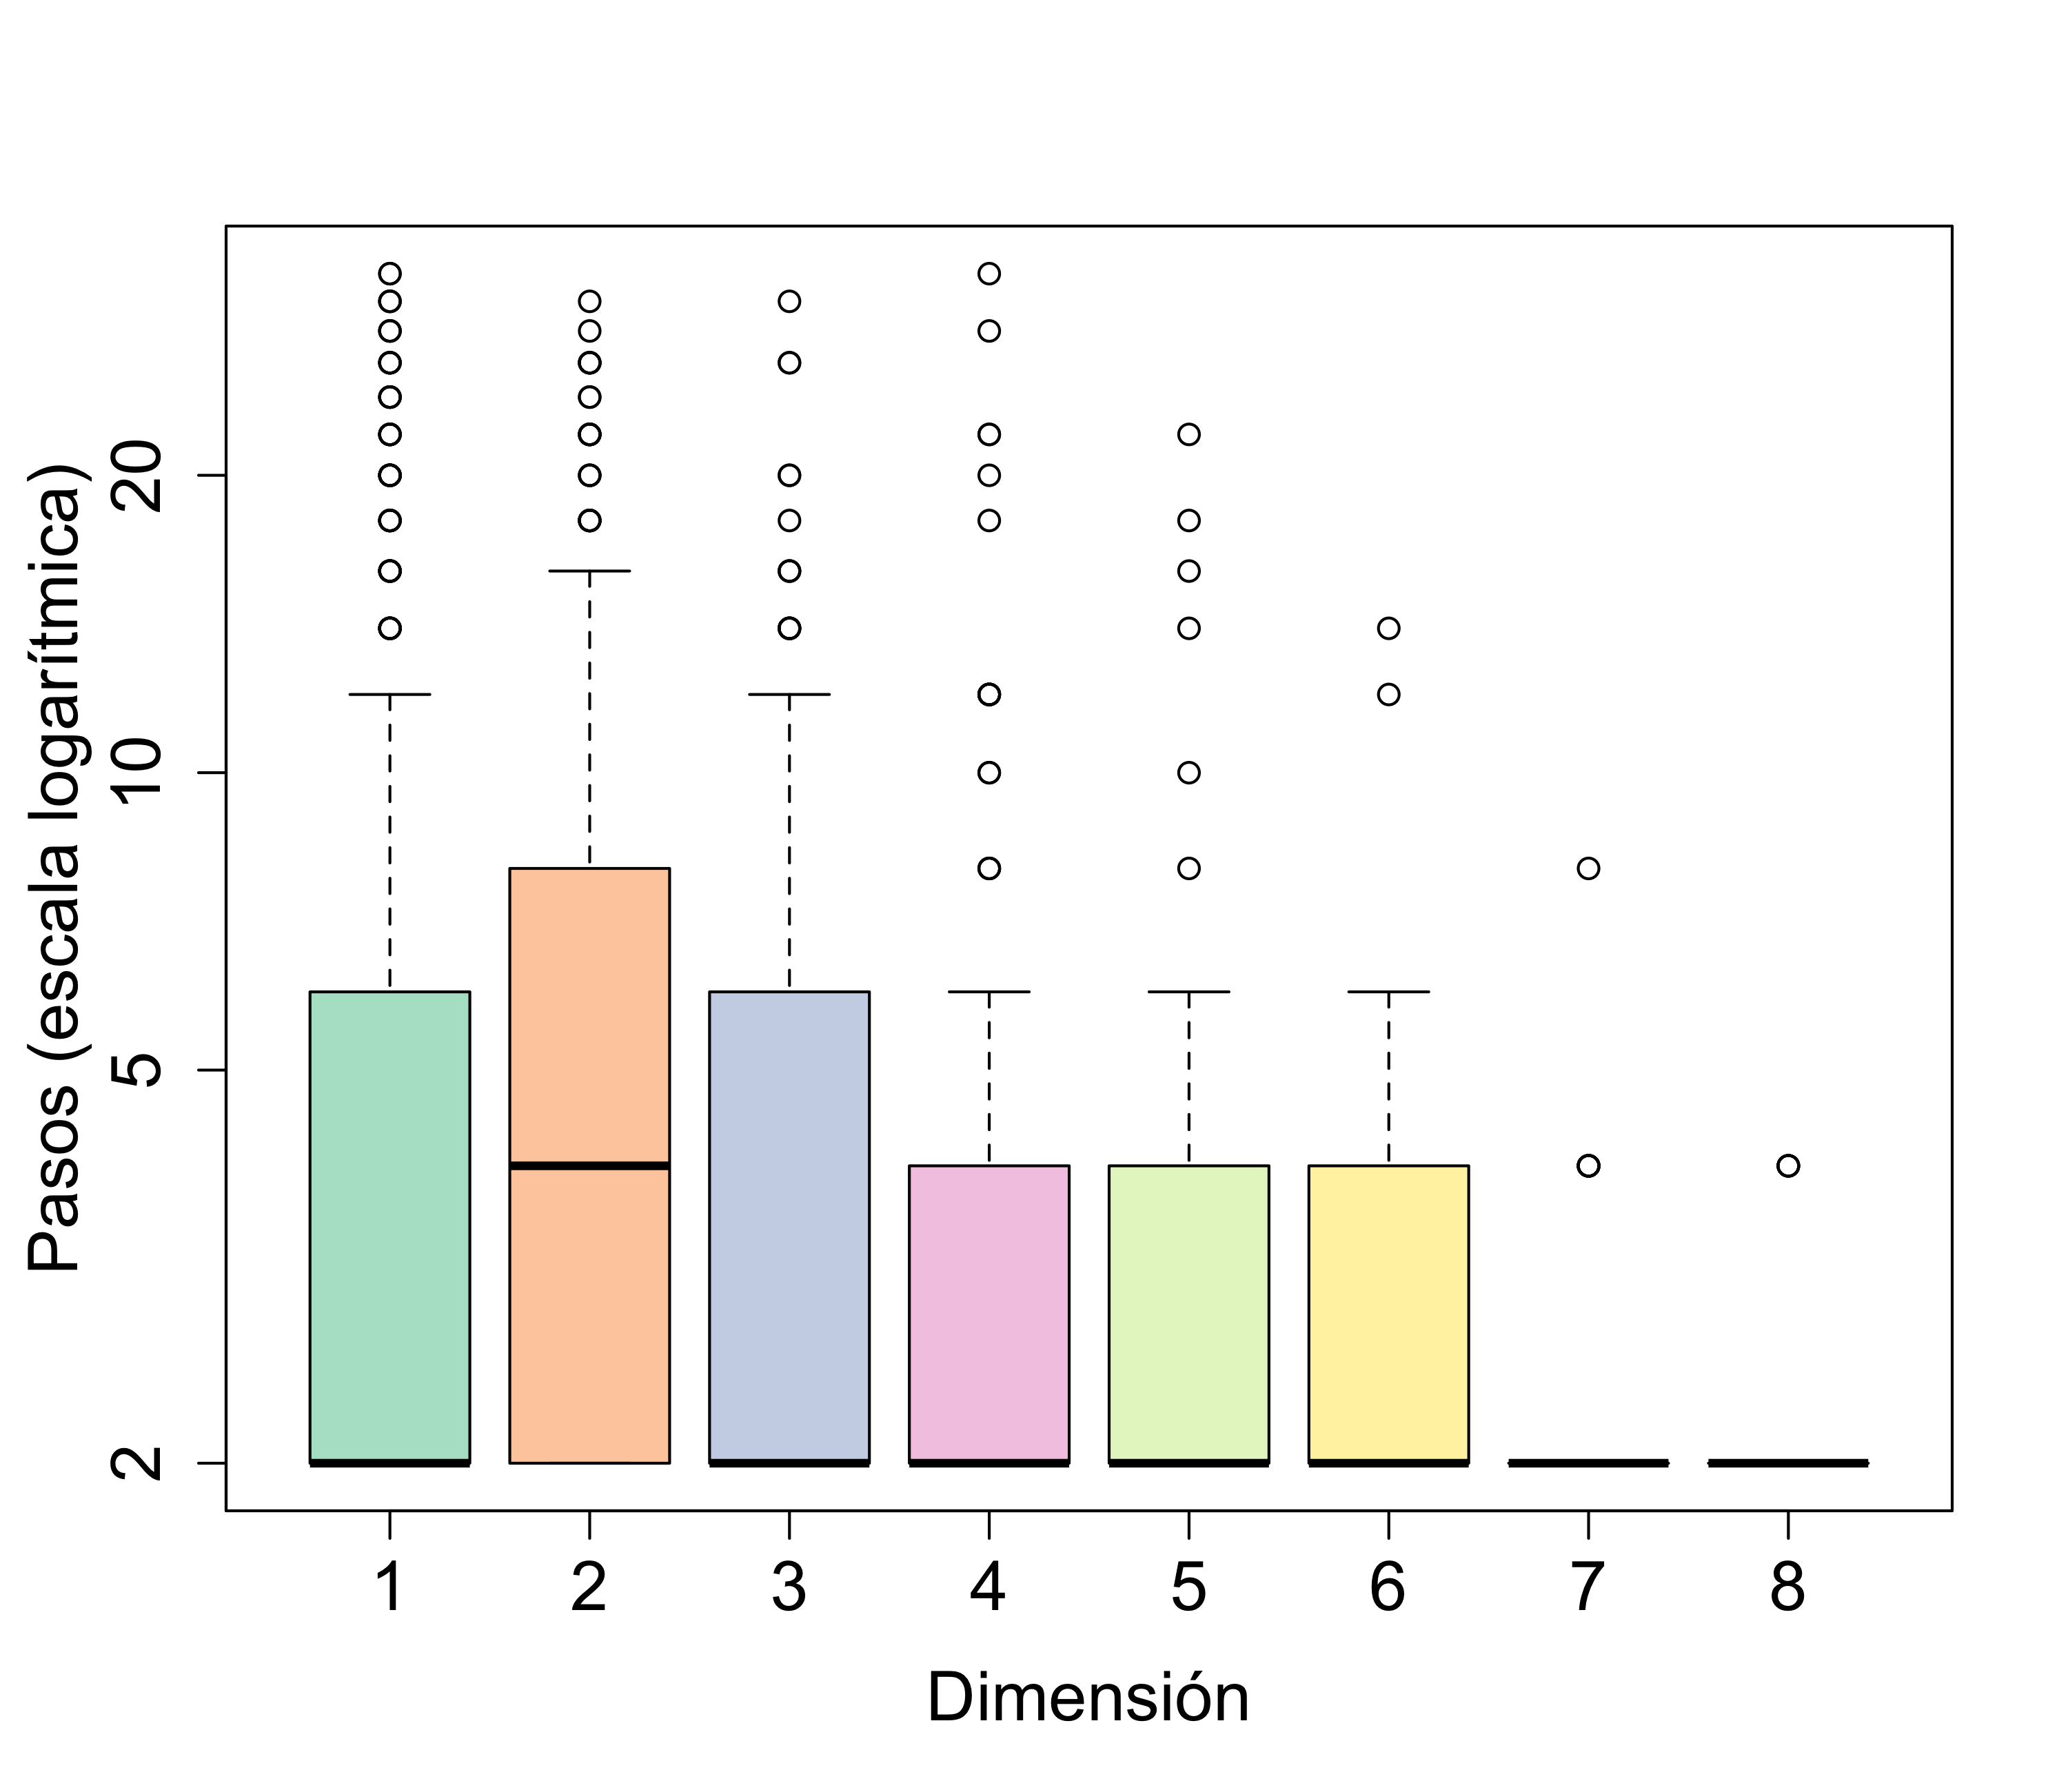
\includegraphics[width=\linewidth]{Largo32-pasos.png}
 		 \caption{Caminata de 32 pasos.}
 		\label{32pasos}
 	\end{subfigure}
 	\begin{subfigure}[b]{0.45\linewidth}
 		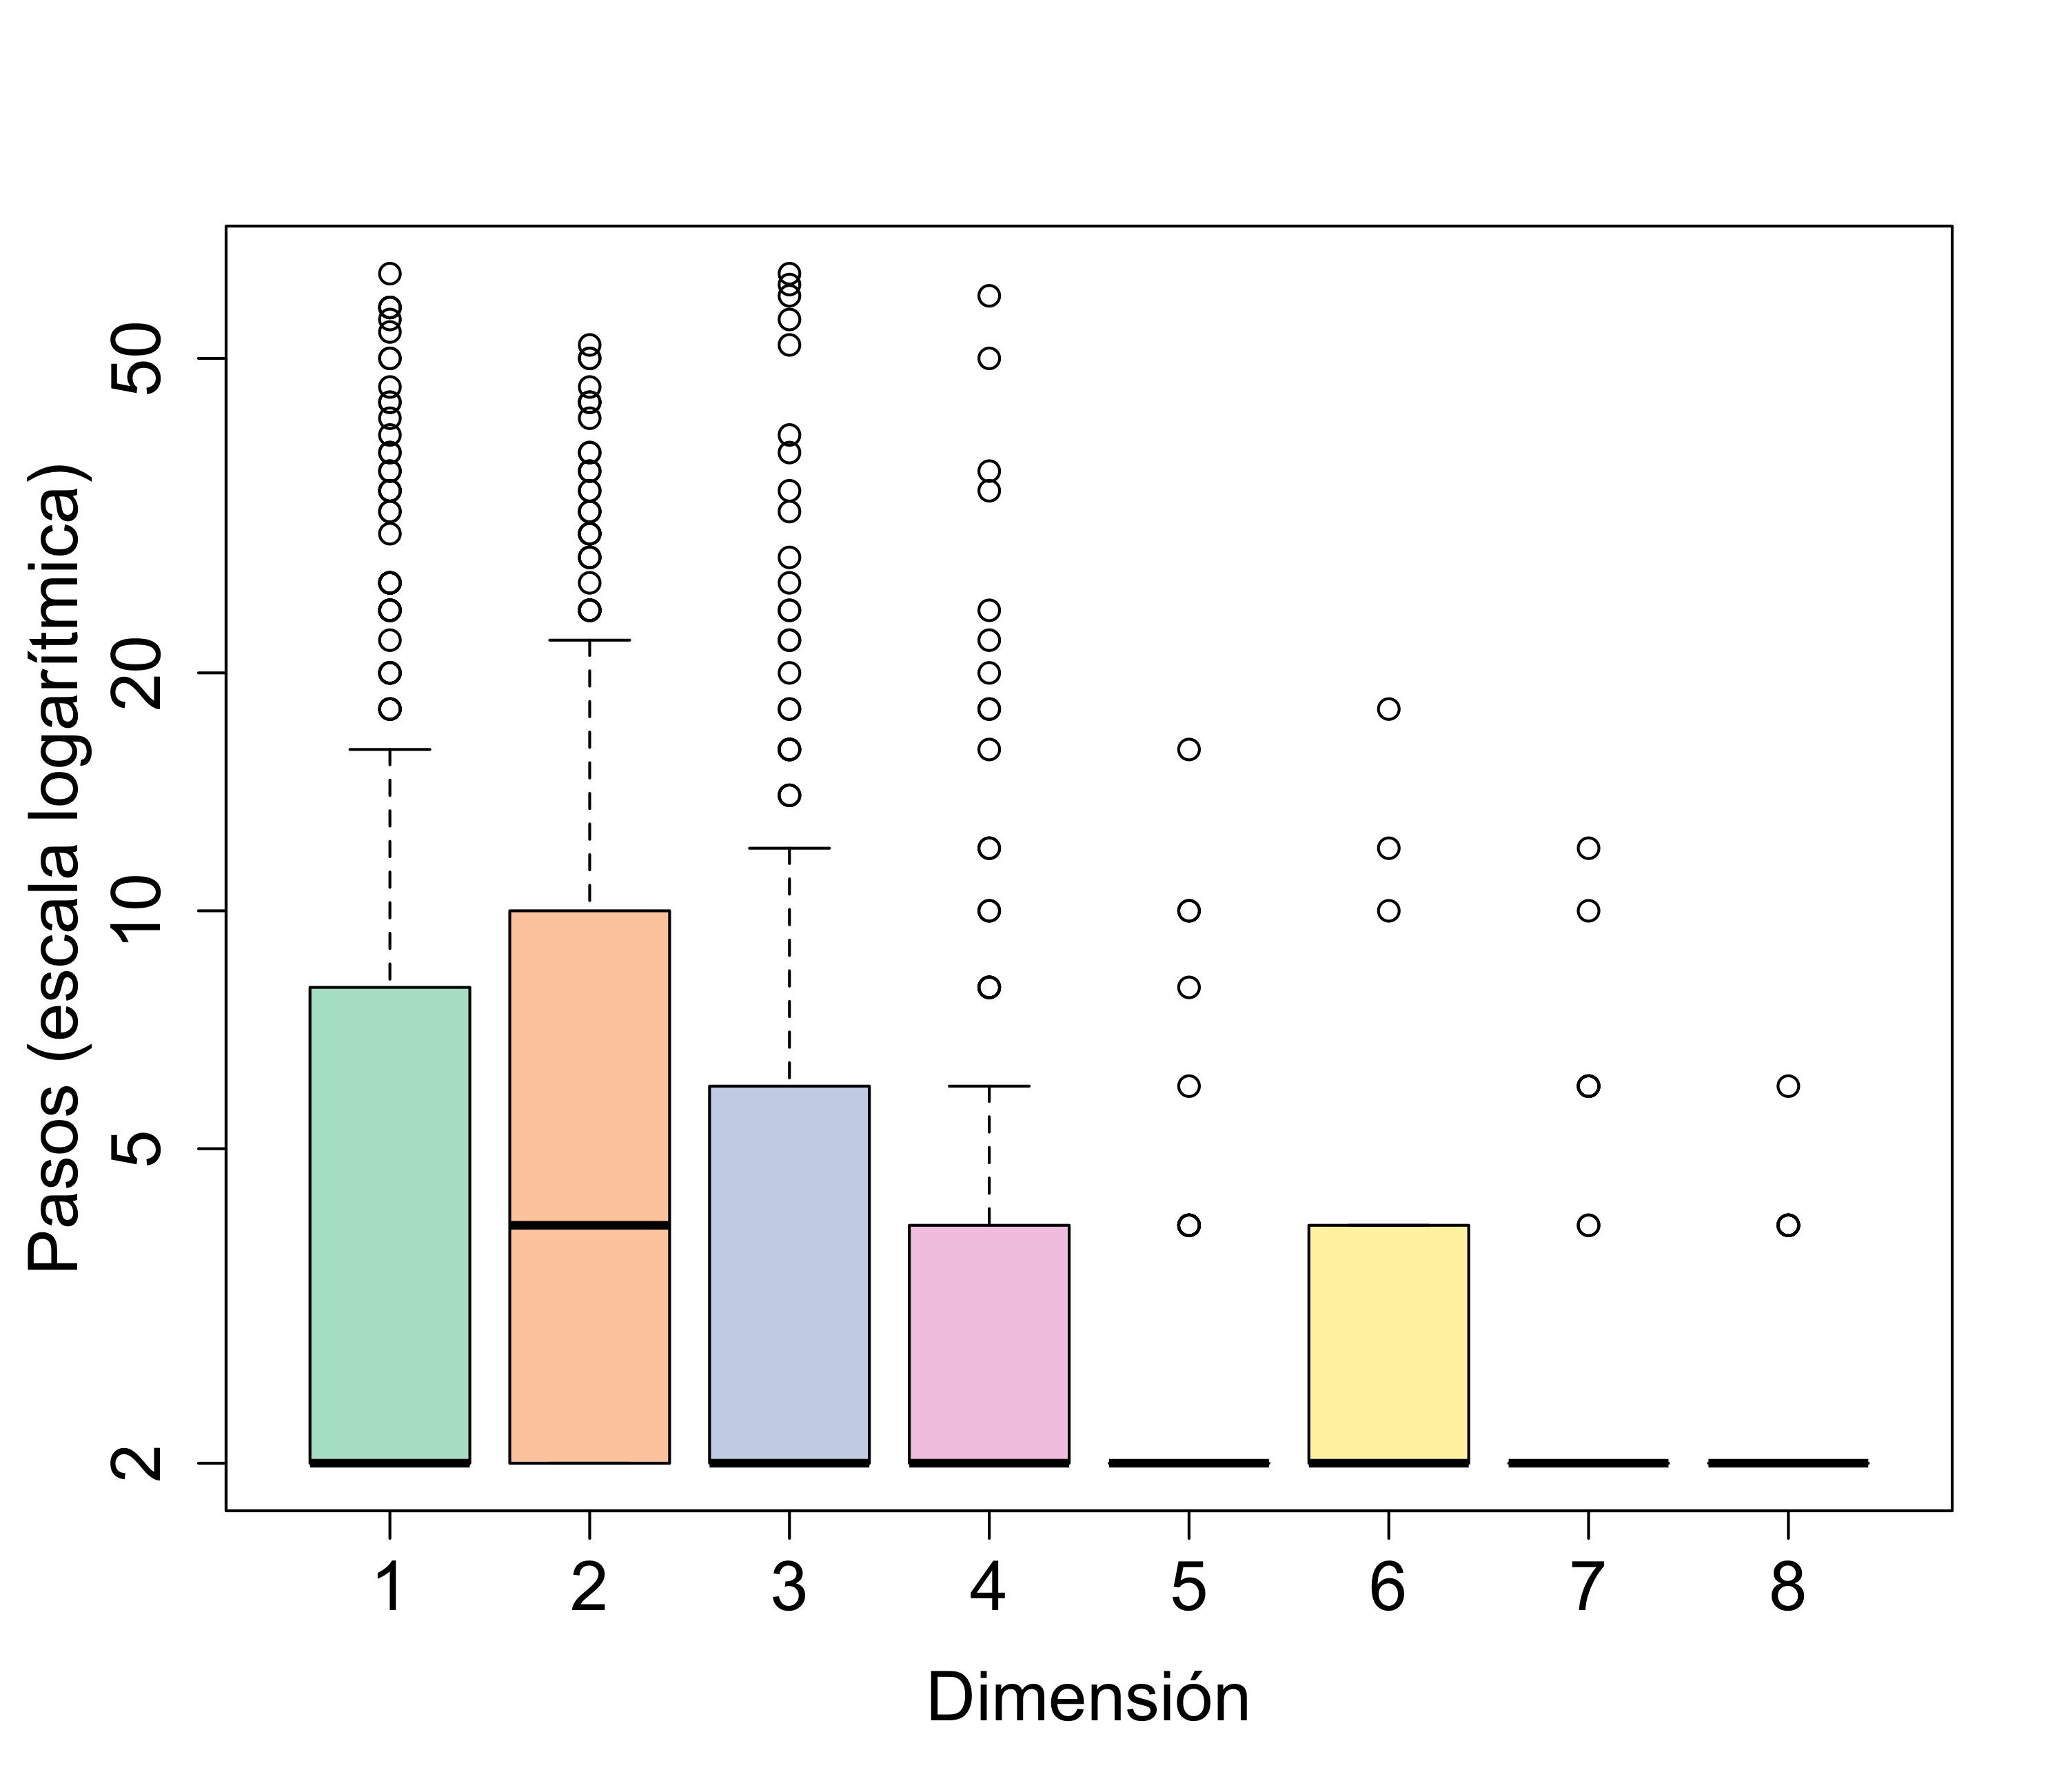
\includegraphics[width=\linewidth]{Largo64-pasos.png}
 		 \caption{Caminata de 64 pasos.}
 		\label{64pasos}
 	\end{subfigure}
 	\begin{subfigure}[b]{0.45\linewidth}
 		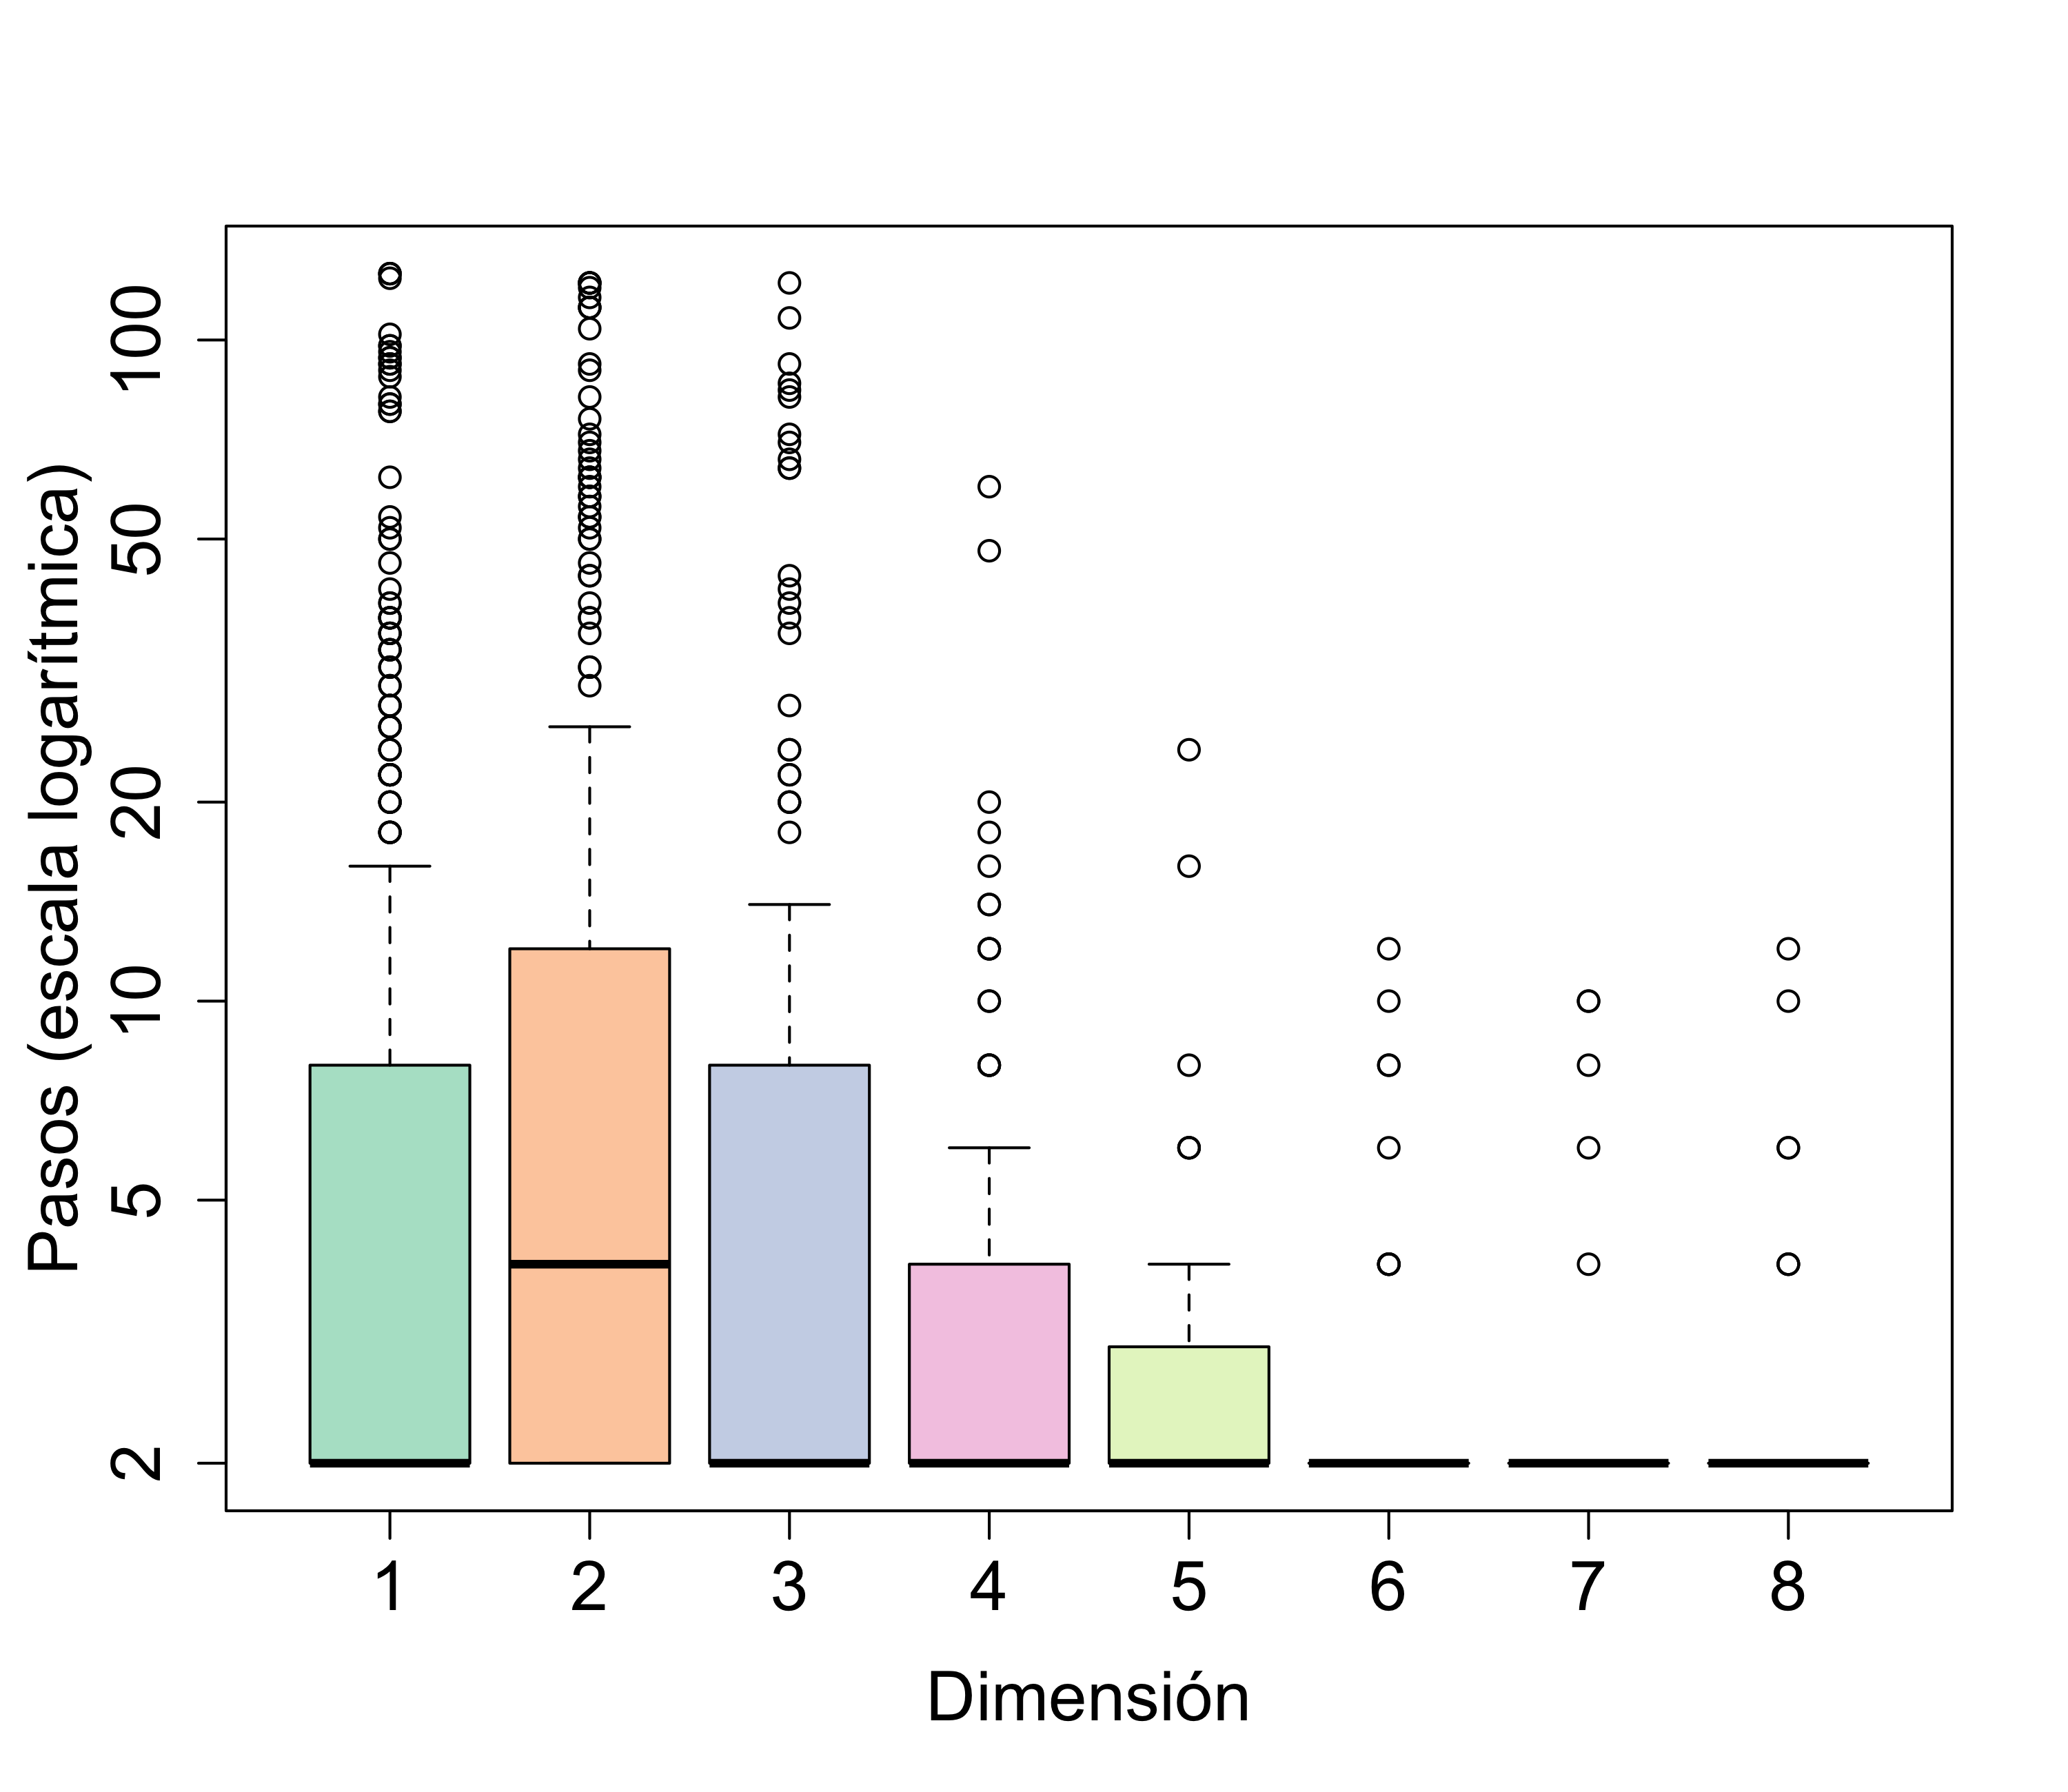
\includegraphics[width=\linewidth]{Largo128-pasos.png}
 		\caption{Caminata de 128 pasos.}
 		\label{128pasos}
 	\end{subfigure}
	\begin{subfigure}[b]{0.45\linewidth}
 		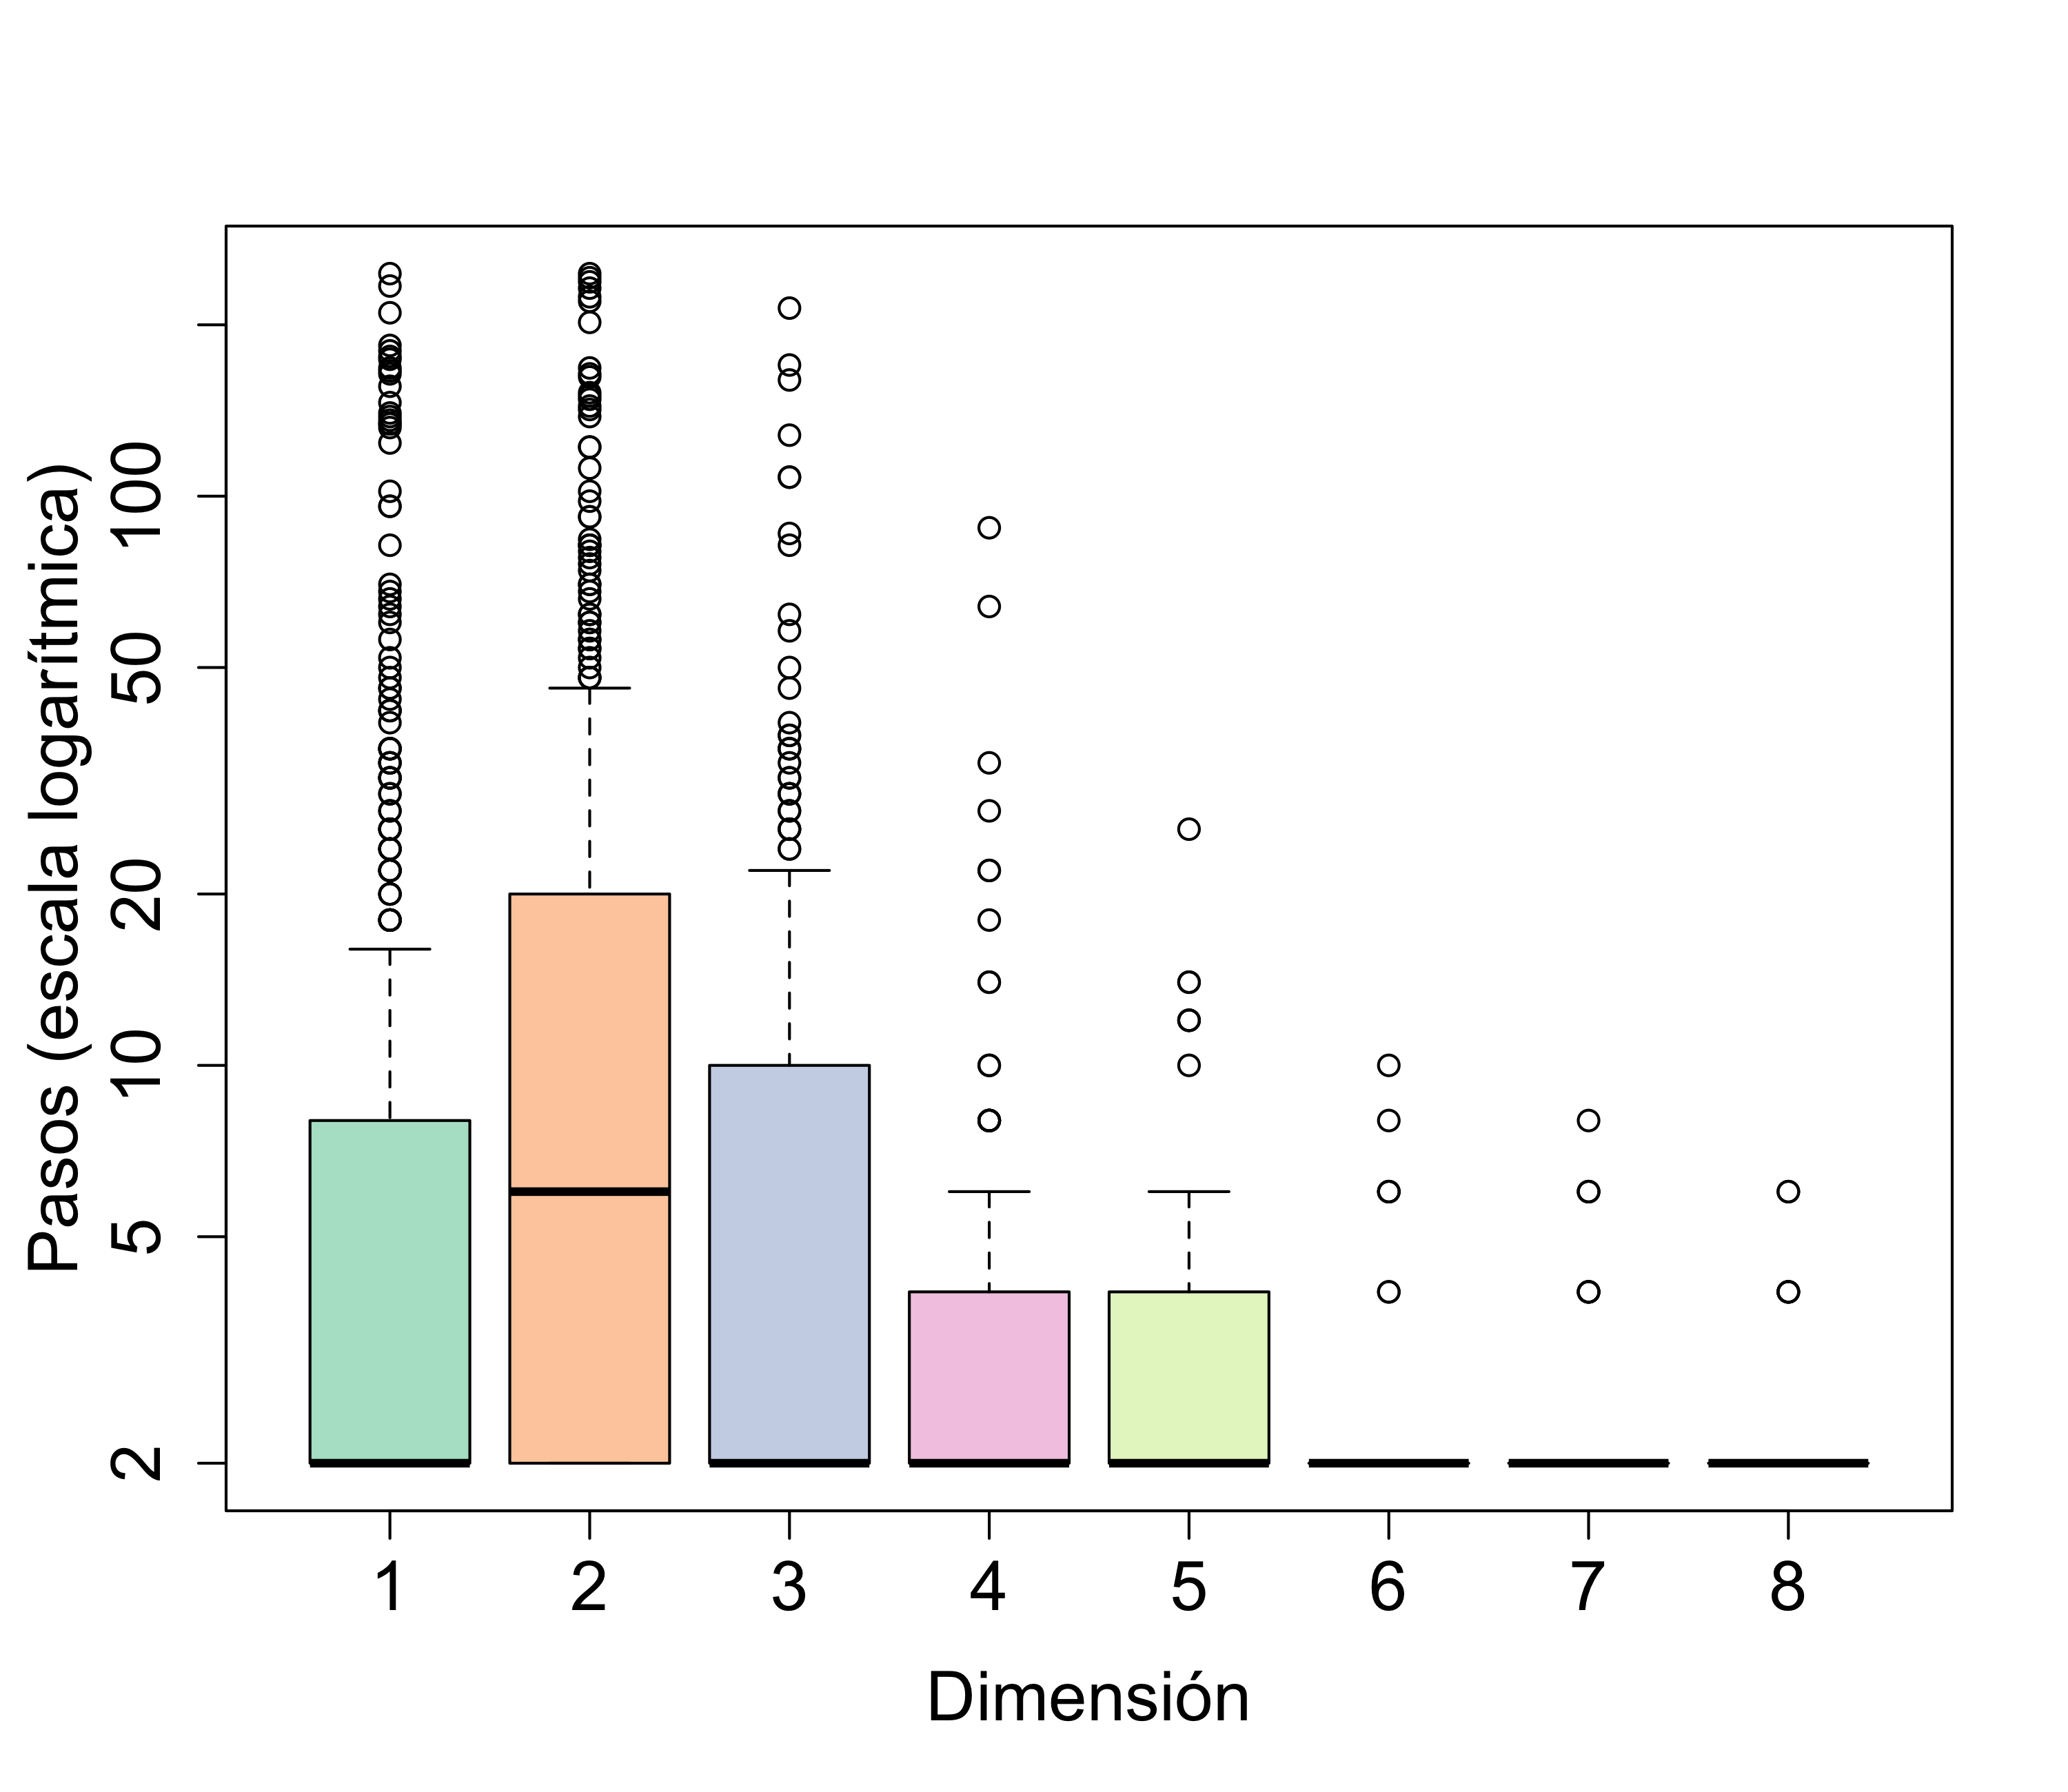
\includegraphics[width=\linewidth]{Largo256-pasos.png}
 		 \caption{Caminata de 256 pasos.}
 		\label{256pasos}
 	\end{subfigure}
 		\begin{subfigure}[b]{0.45\linewidth}
 		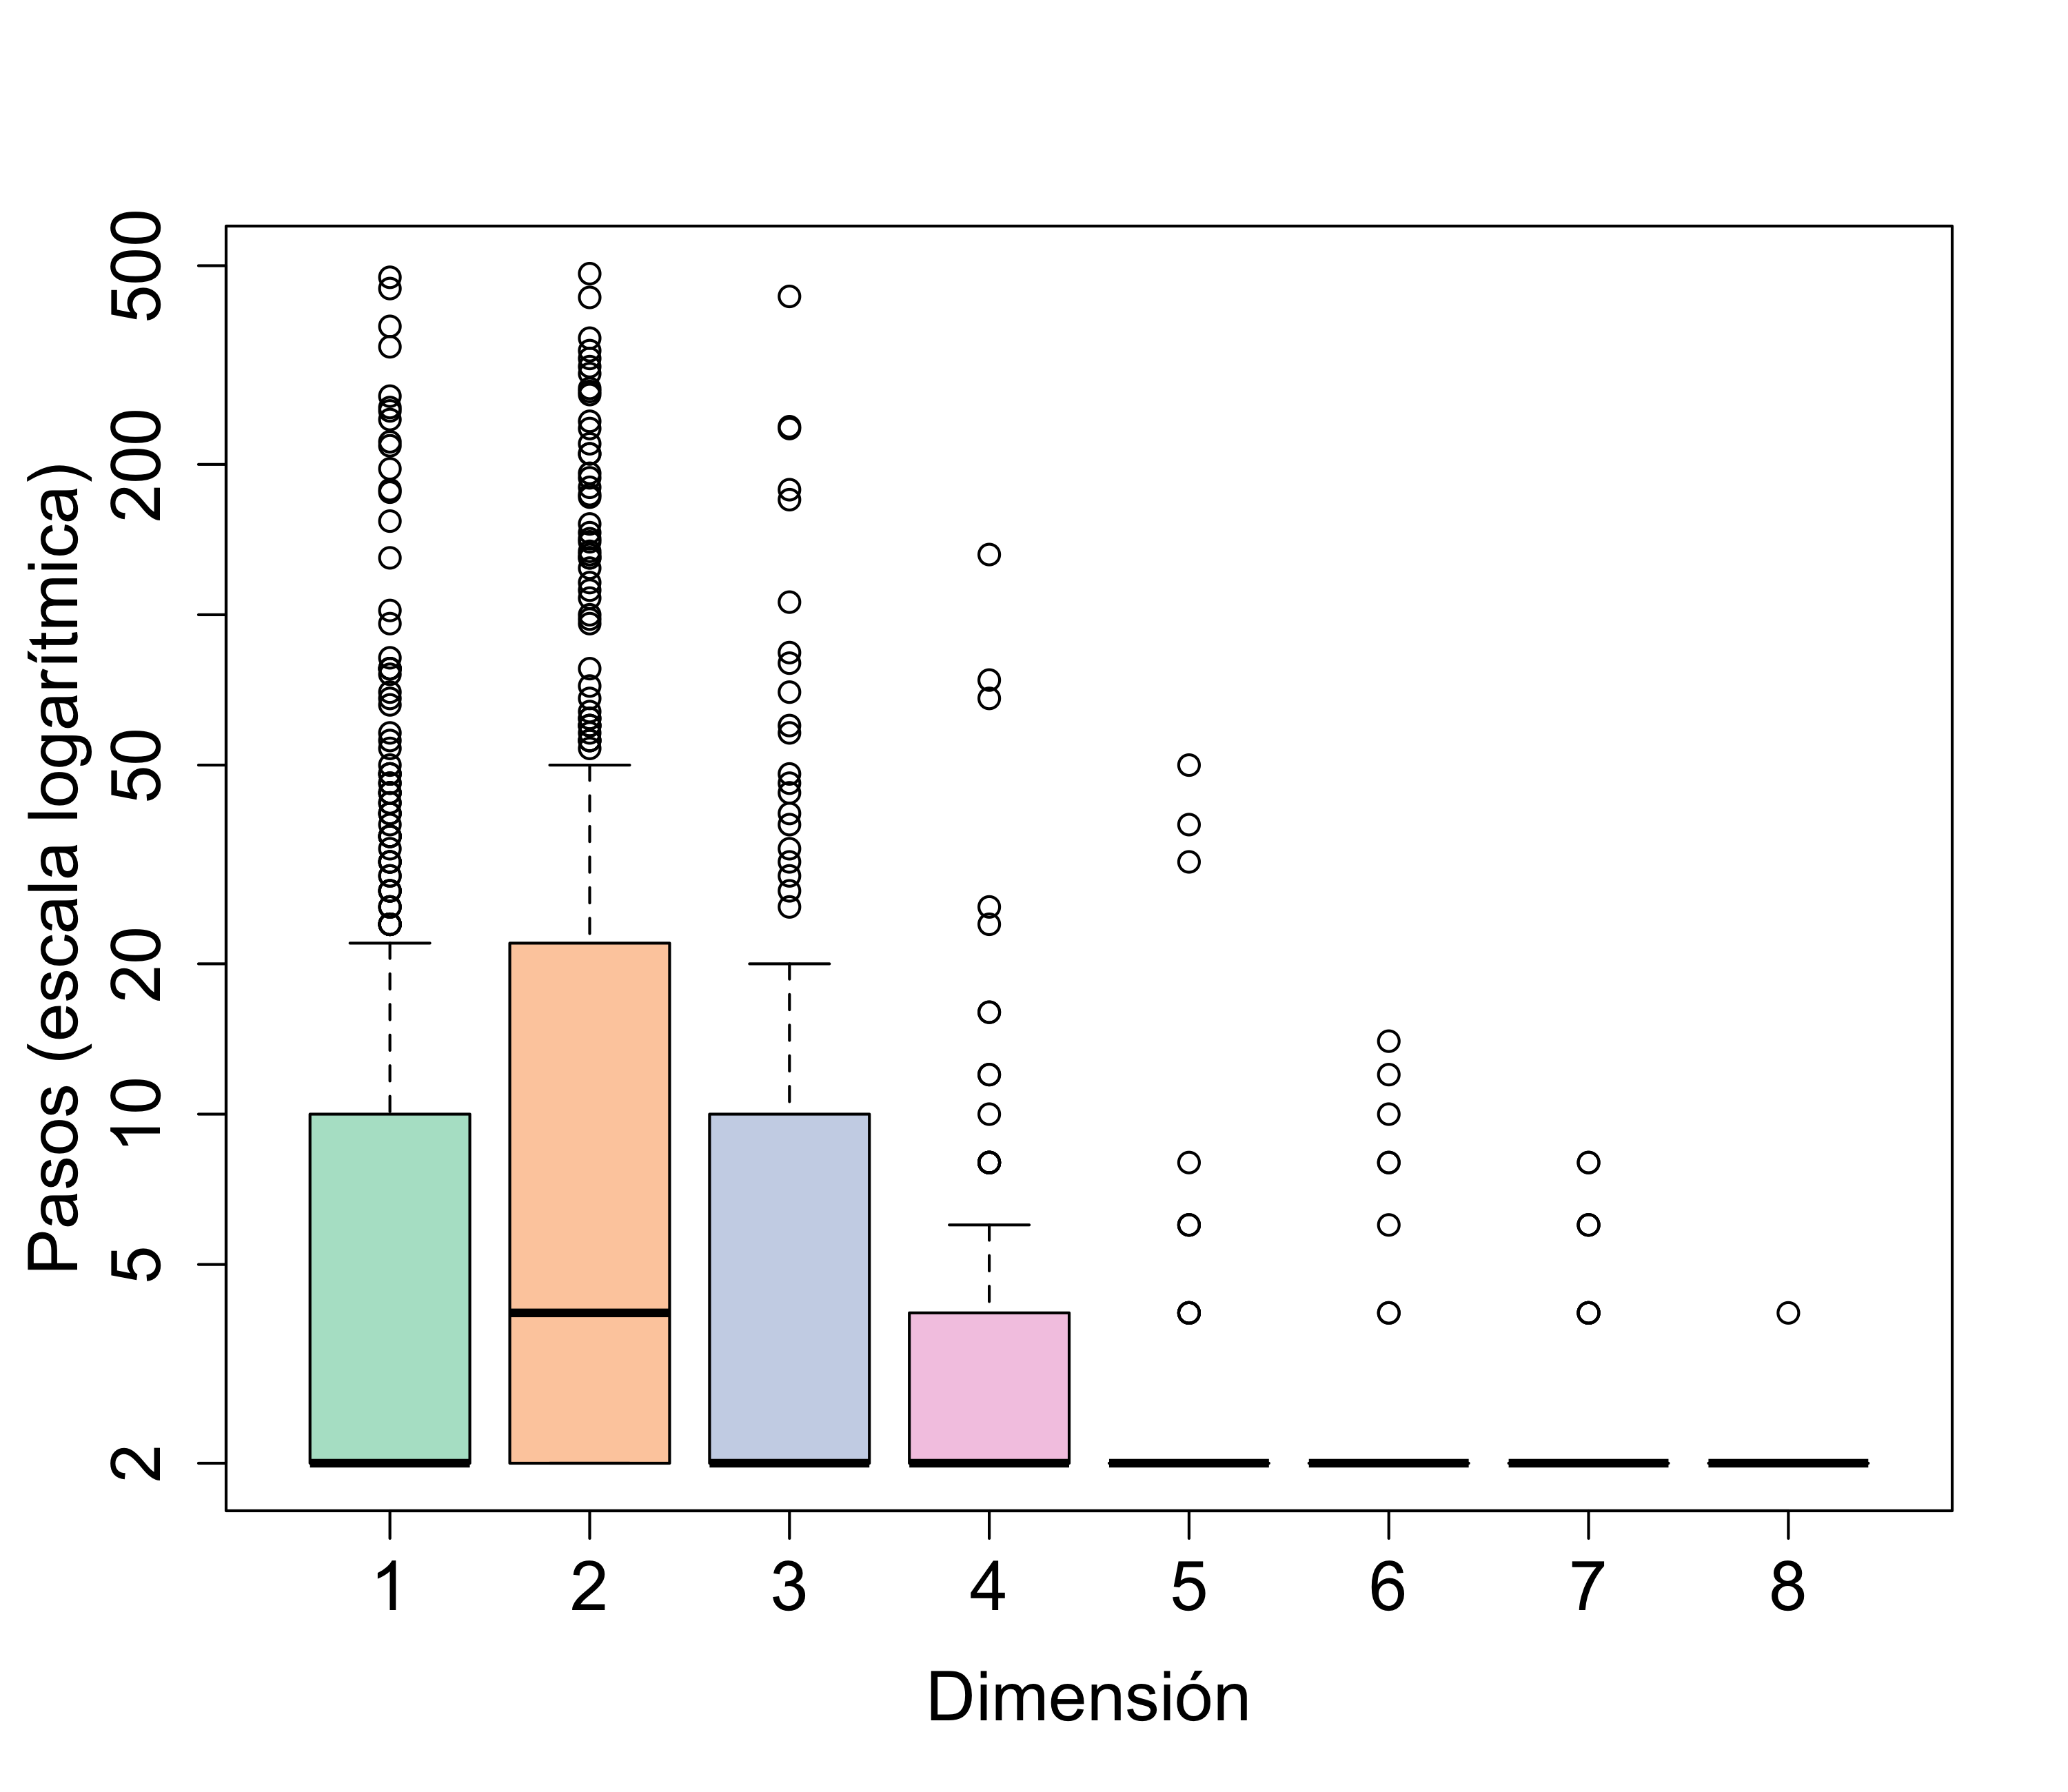
\includegraphics[width=\linewidth]{Largo512-pasos.png}
 		 \caption{Caminata de 512 pasos.}
 		\label{512pasos}
 	\end{subfigure}
 		\begin{subfigure}[b]{0.45\linewidth}
 		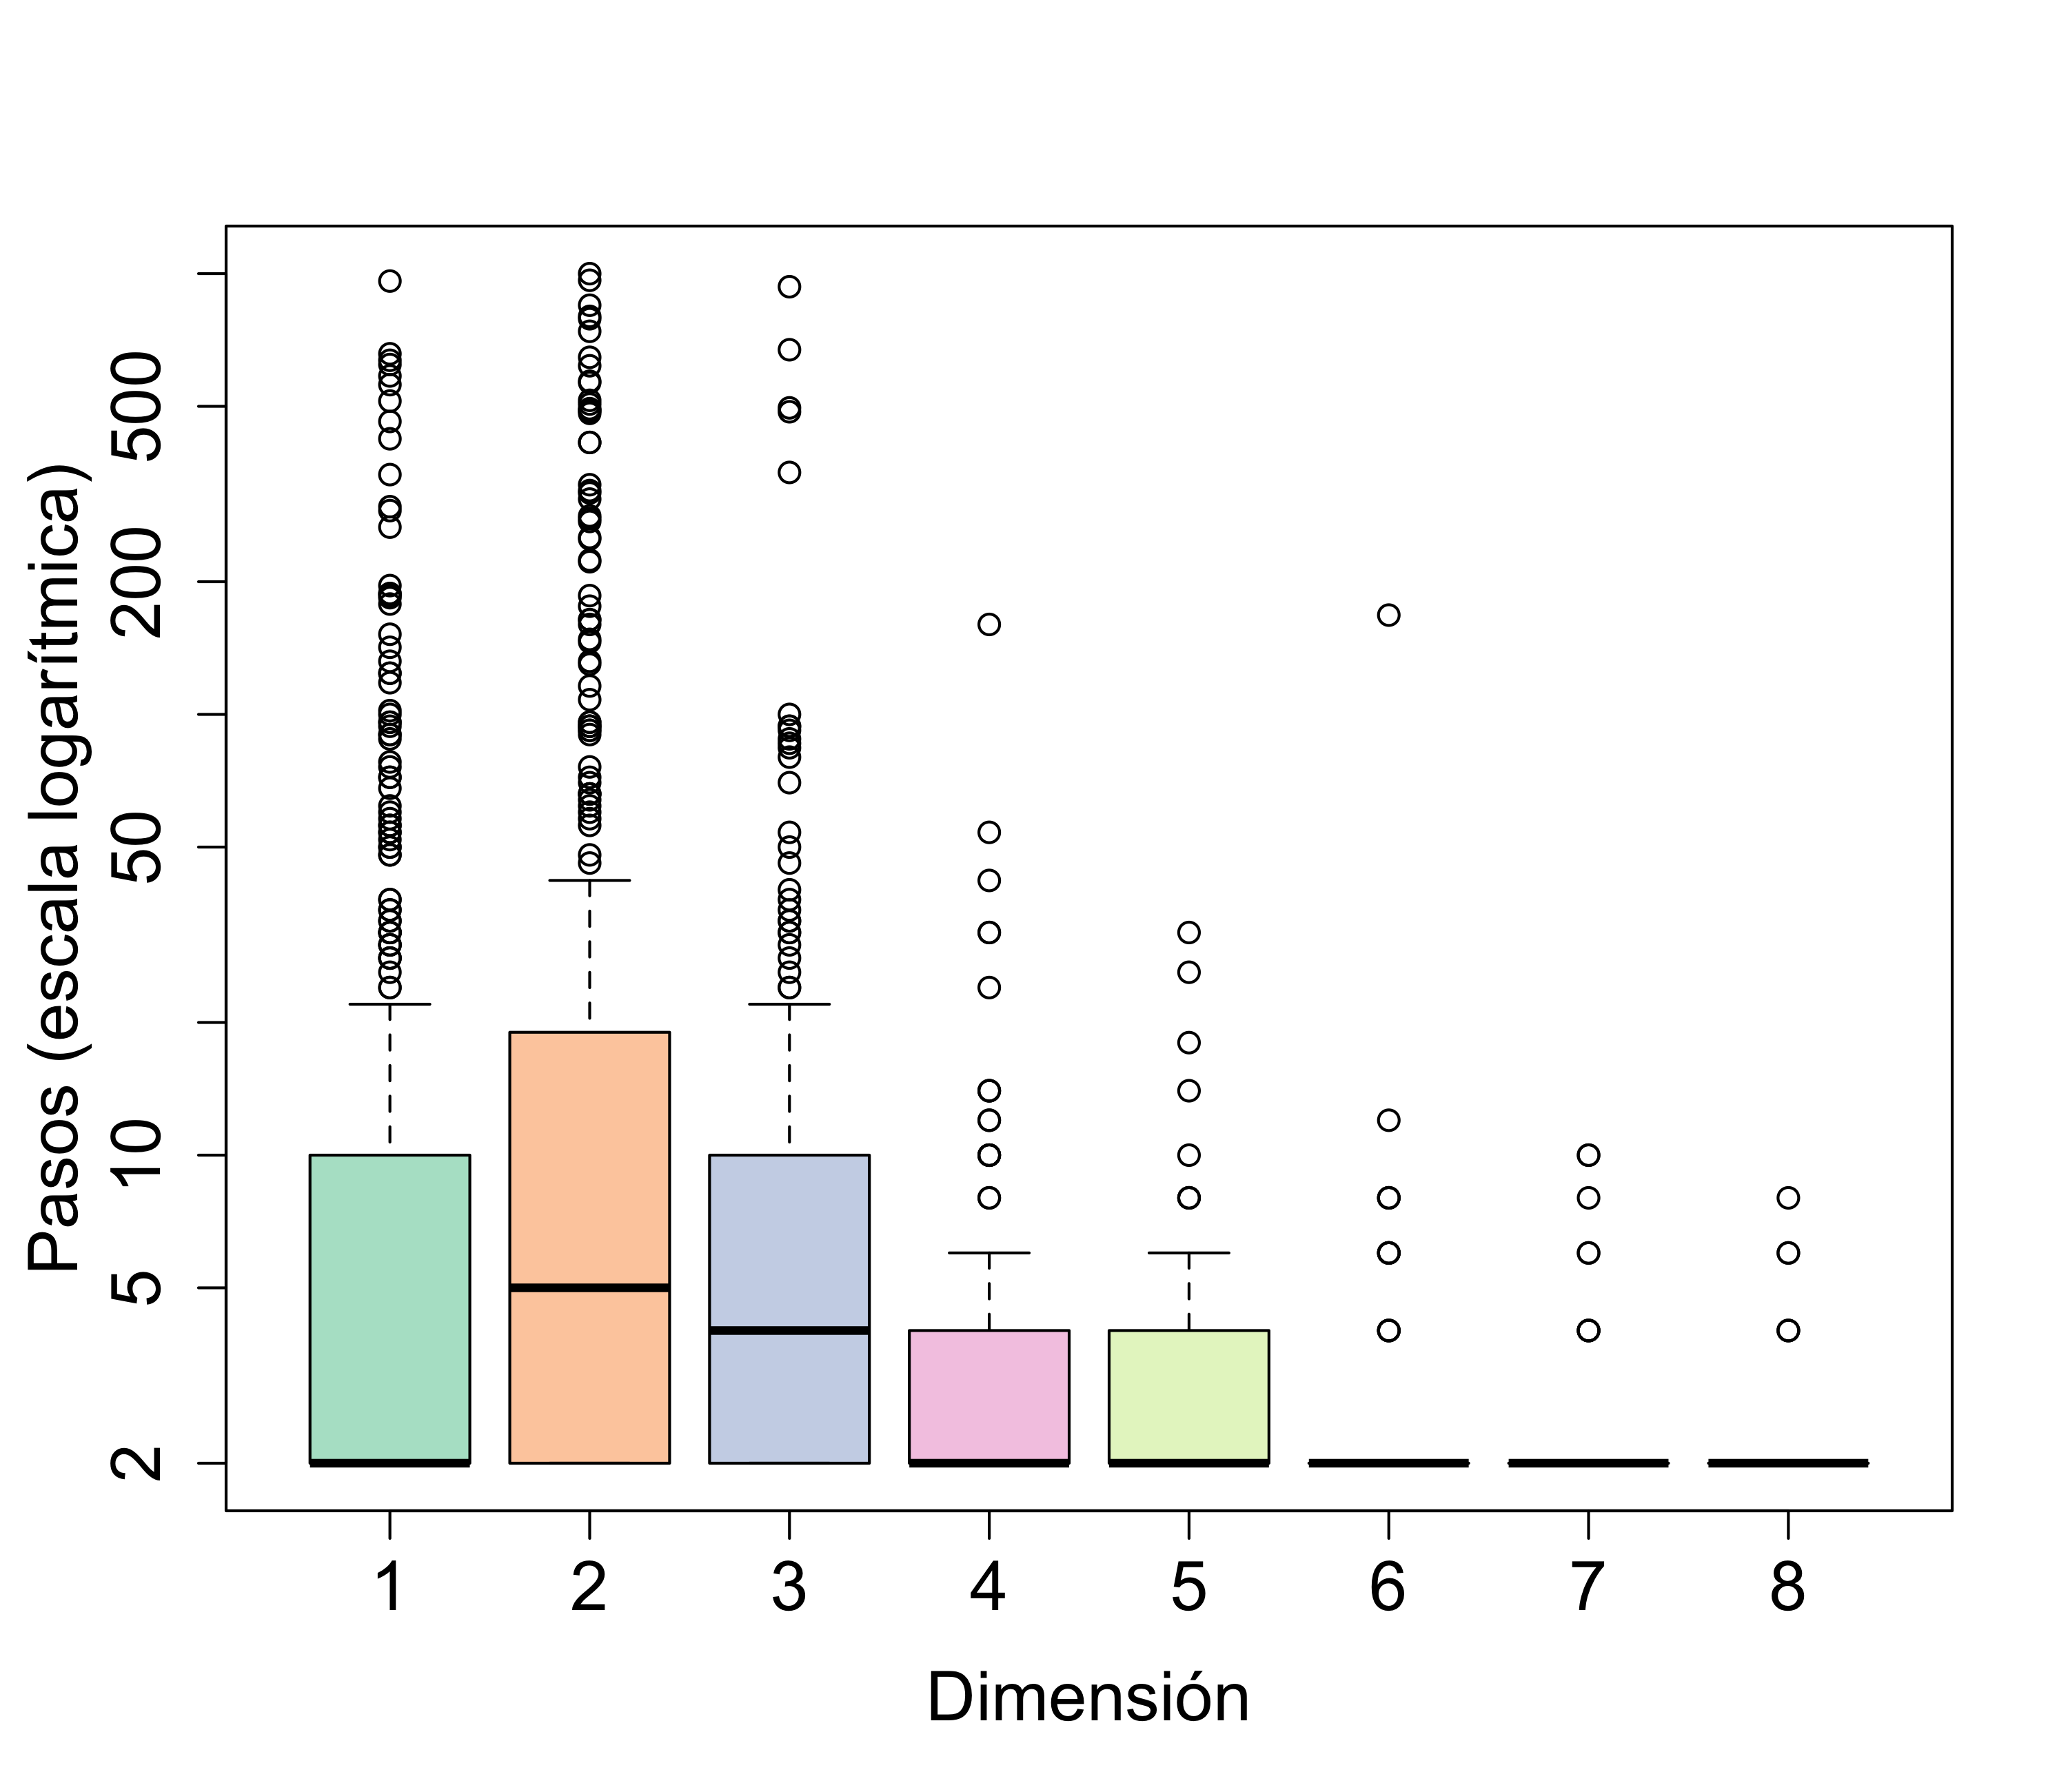
\includegraphics[width=\linewidth]{Largo1024-pasos.png}
 		\caption{Caminata de 1024 pasos.}
 		\label{1024pasos}
 		\end{subfigure}
 	\caption{Pasos de regreso al origen en escala logarítmica.}  		
\label{pasos-log}
 \end{figure}
 
 
 
 \section{Reto 1}
 El primer reto es estudiar de forma sistemática y automatizada el tiempo de ejecución de una caminata (en milisegundos) en términos del largo de la caminata (en pasos) y la dimensión \cite{elisa}. 
 
 En la figura \ref{tiempo-largos}, se muestra las gráficas de barras correspondientes a la duración de una caminata variando la dimensión en la que se lleva a cabo. Se aprecia que mientras la longitud incrementa, la altura de las barras se ve uniforme, por lo que se concluye que la dimensión en la que se mueve la partícula no afecta el tiempo de la caminata.
 
 En la figura \ref{tiempos-dimension}, se muestra las gráficas correspondientes a la duración de una caminata variando la longitud de esta. Se nota que mientras la longitud incrementa, el tiempo de la caminata aumenta, este comportamiento se aprecia en las ocho dimensiones con las que se trabaja. Por lo que se concluye que la longitud de la caminata sí afecta la duración de la caminata.
 
 
  \begin{figure}
 	\centering
 	\begin{subfigure}[b]{0.45\linewidth}
 		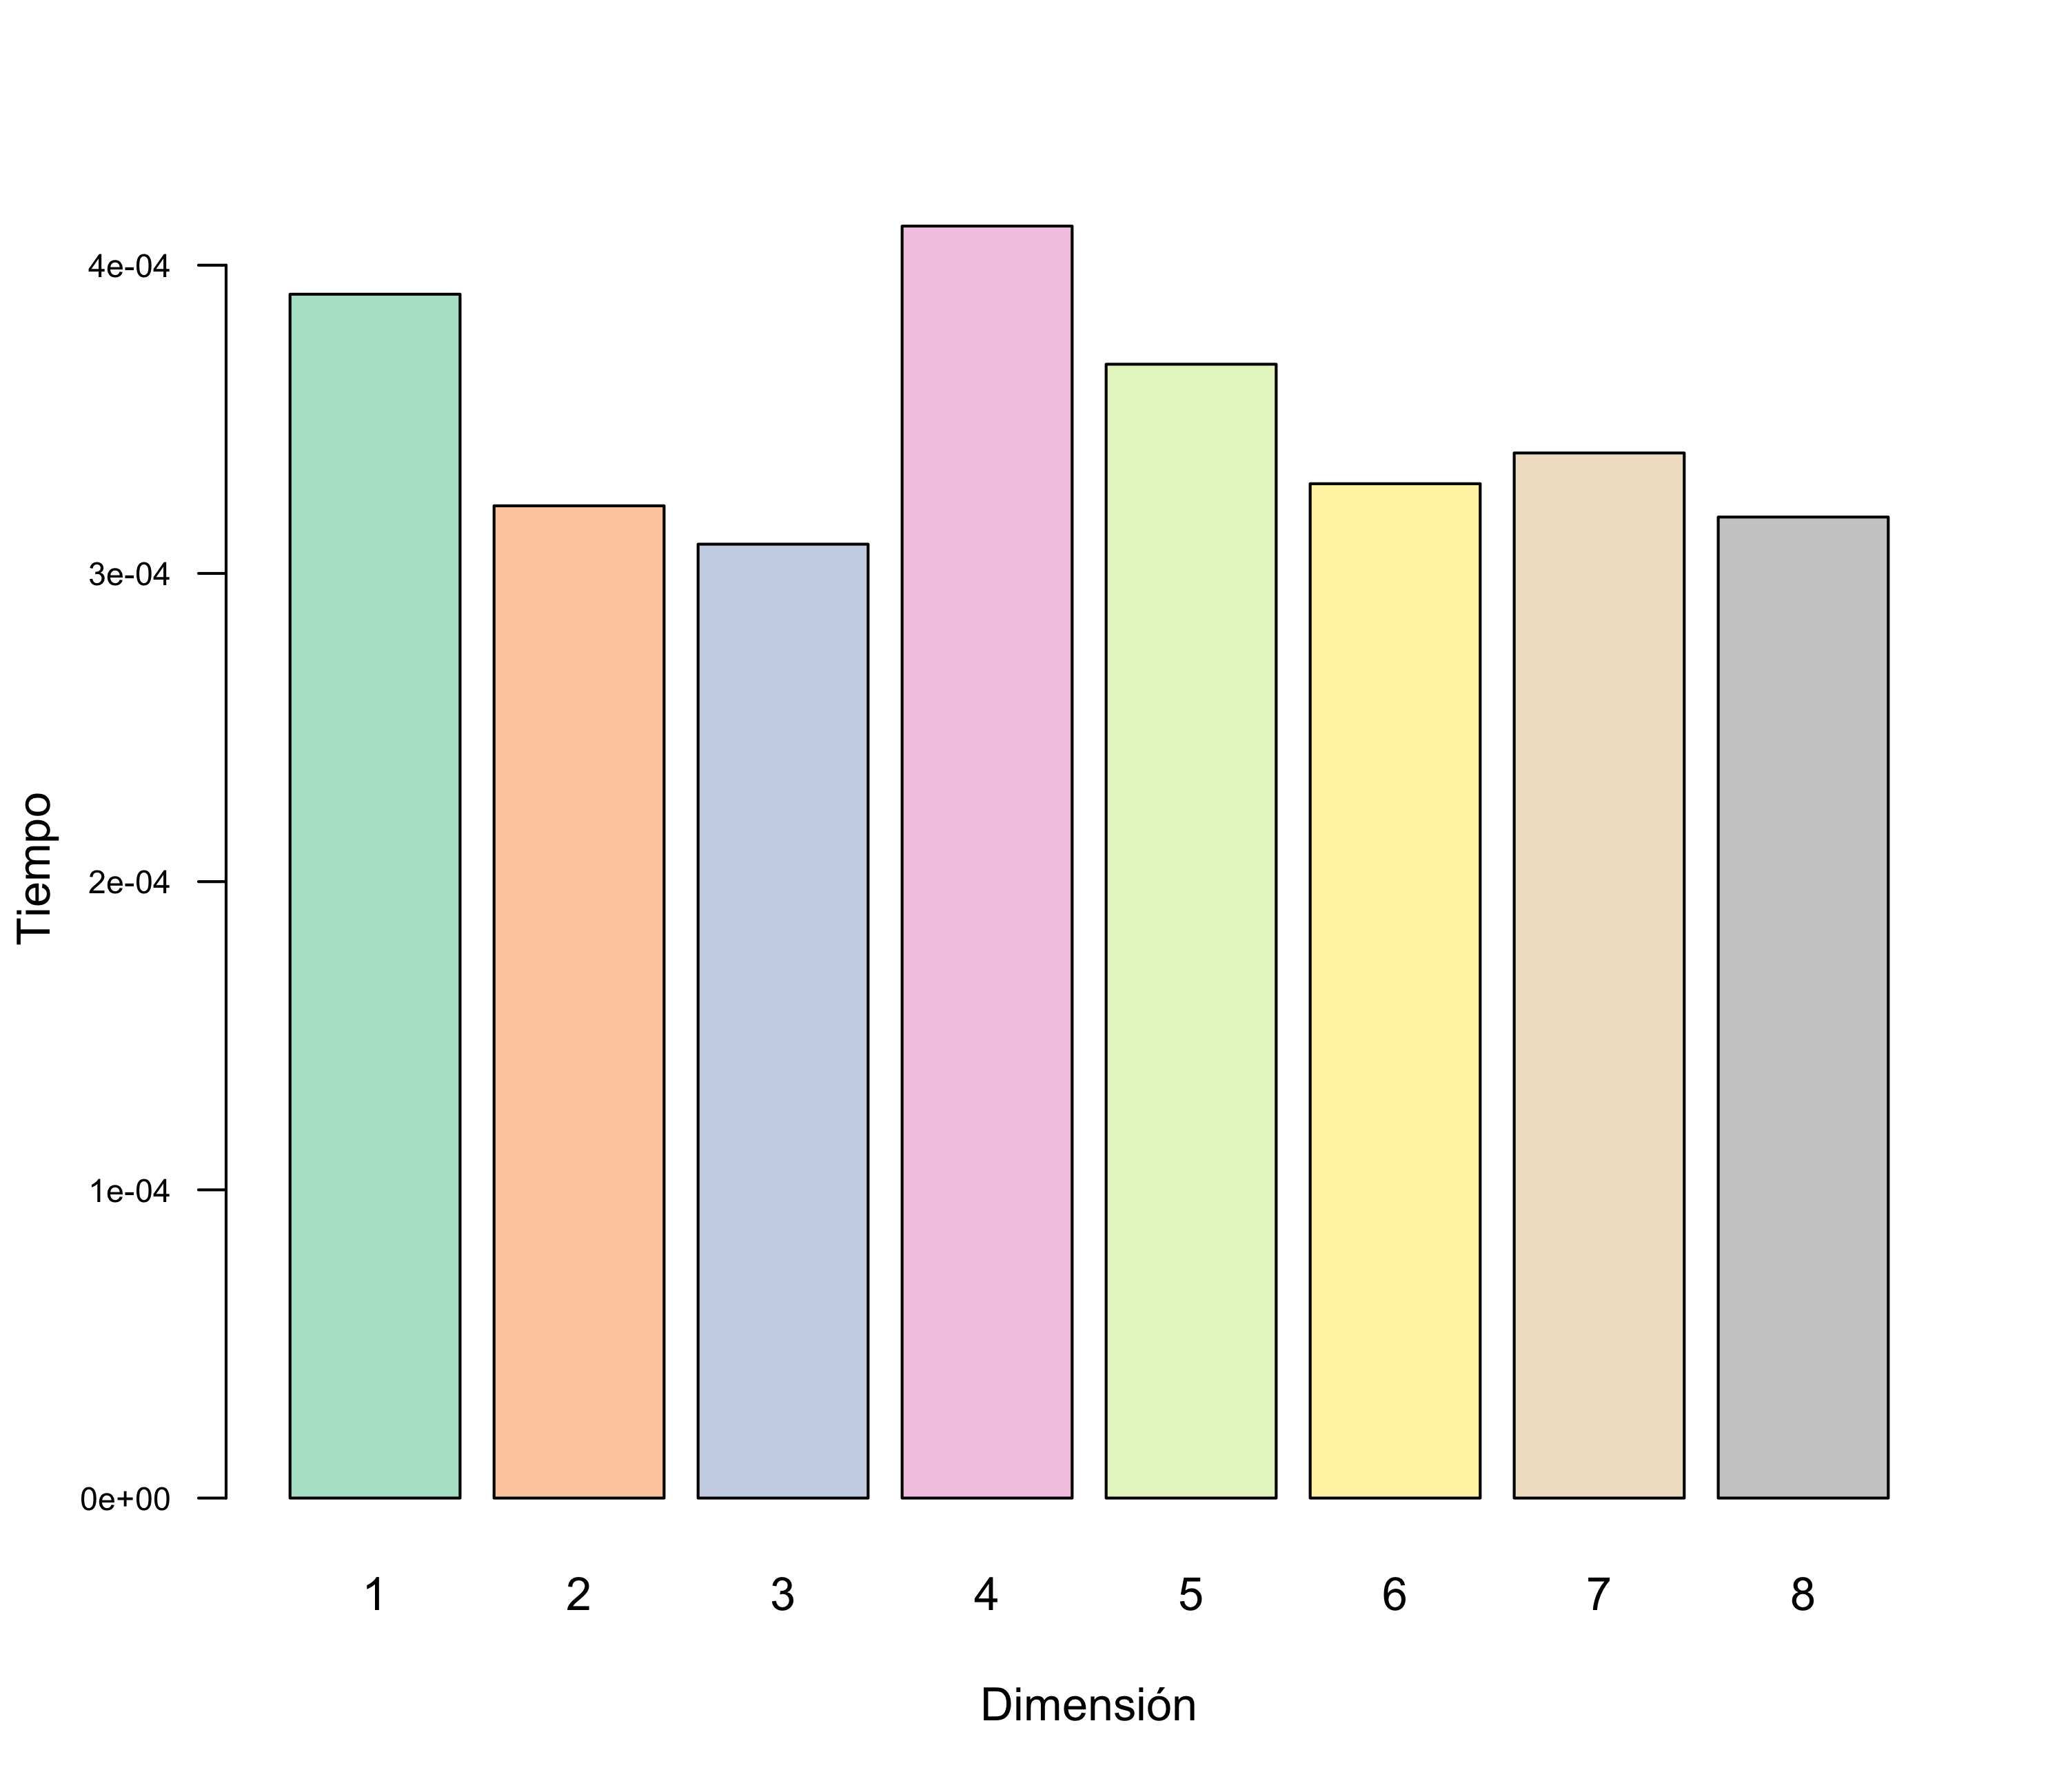
\includegraphics[width=\linewidth]{32-tiempo.png}
 		 \caption{Caminata de 32 pasos.}
 		\label{32tiempo}
 	\end{subfigure}
 	\begin{subfigure}[b]{0.45\linewidth}
 		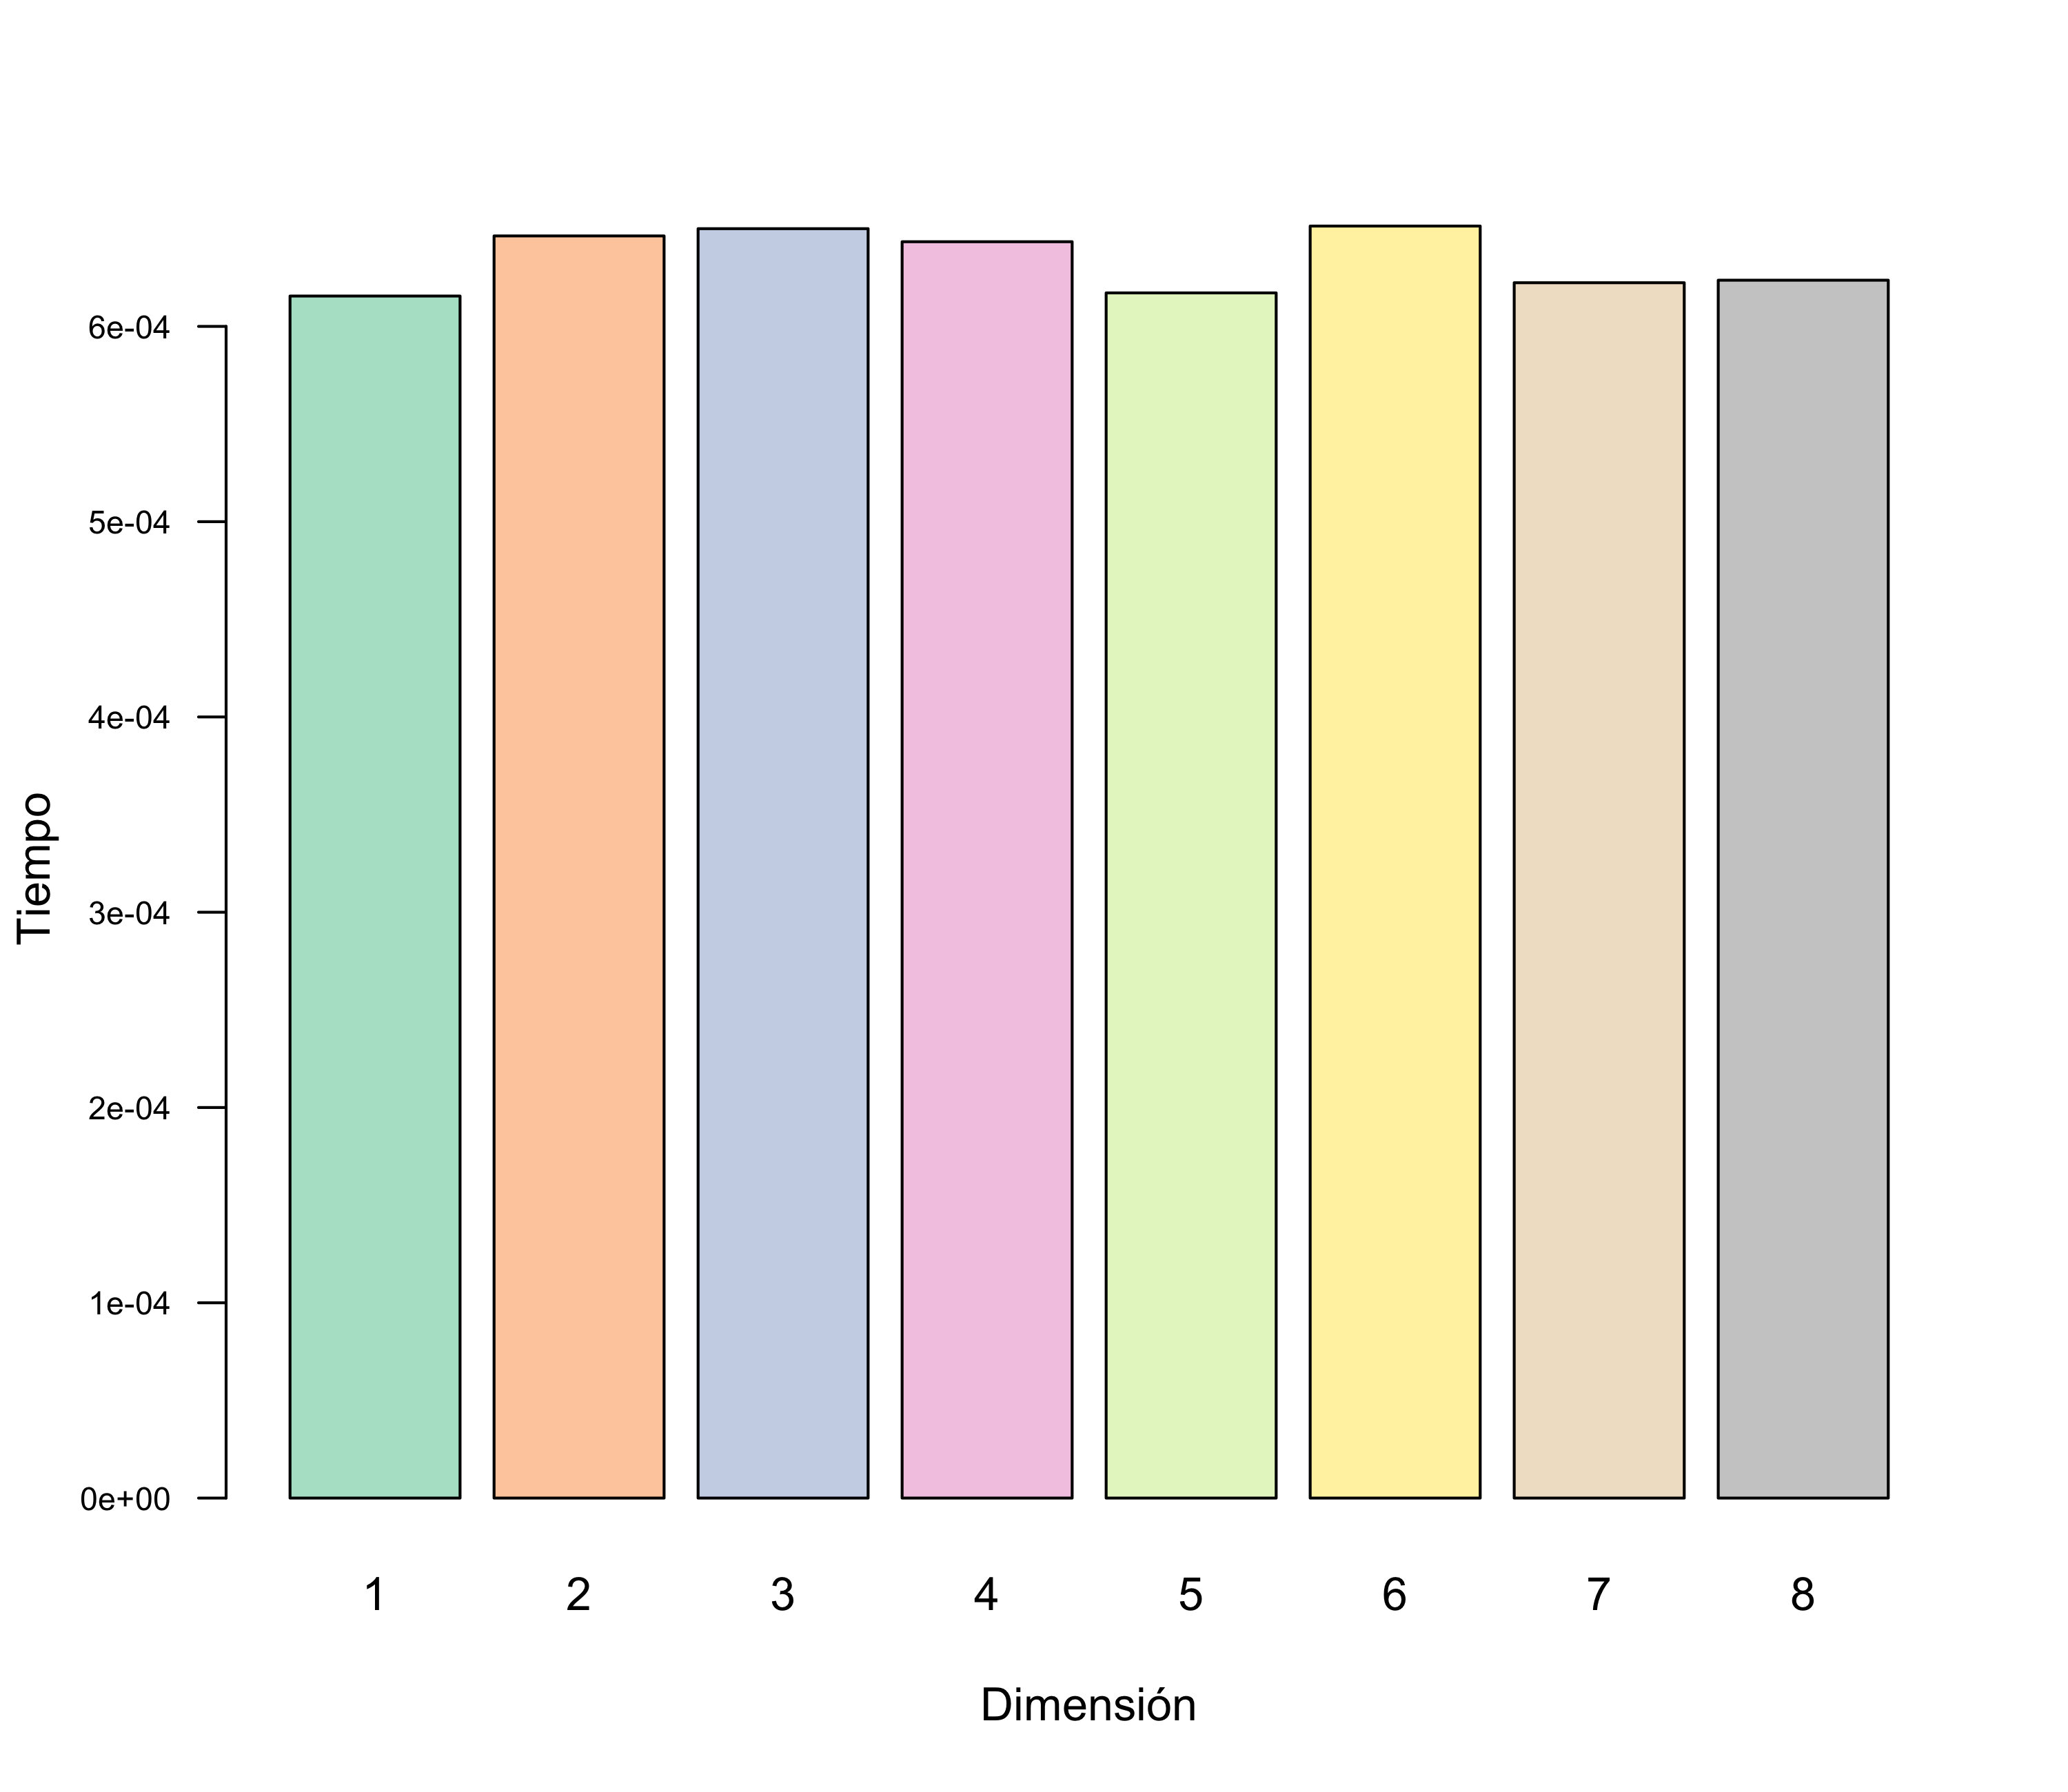
\includegraphics[width=\linewidth]{64-tiempo.png}
 		 \caption{Caminata de 64 pasos.}
 		\label{64tiempo}
 	\end{subfigure}
 	\begin{subfigure}[b]{0.45\linewidth}
 		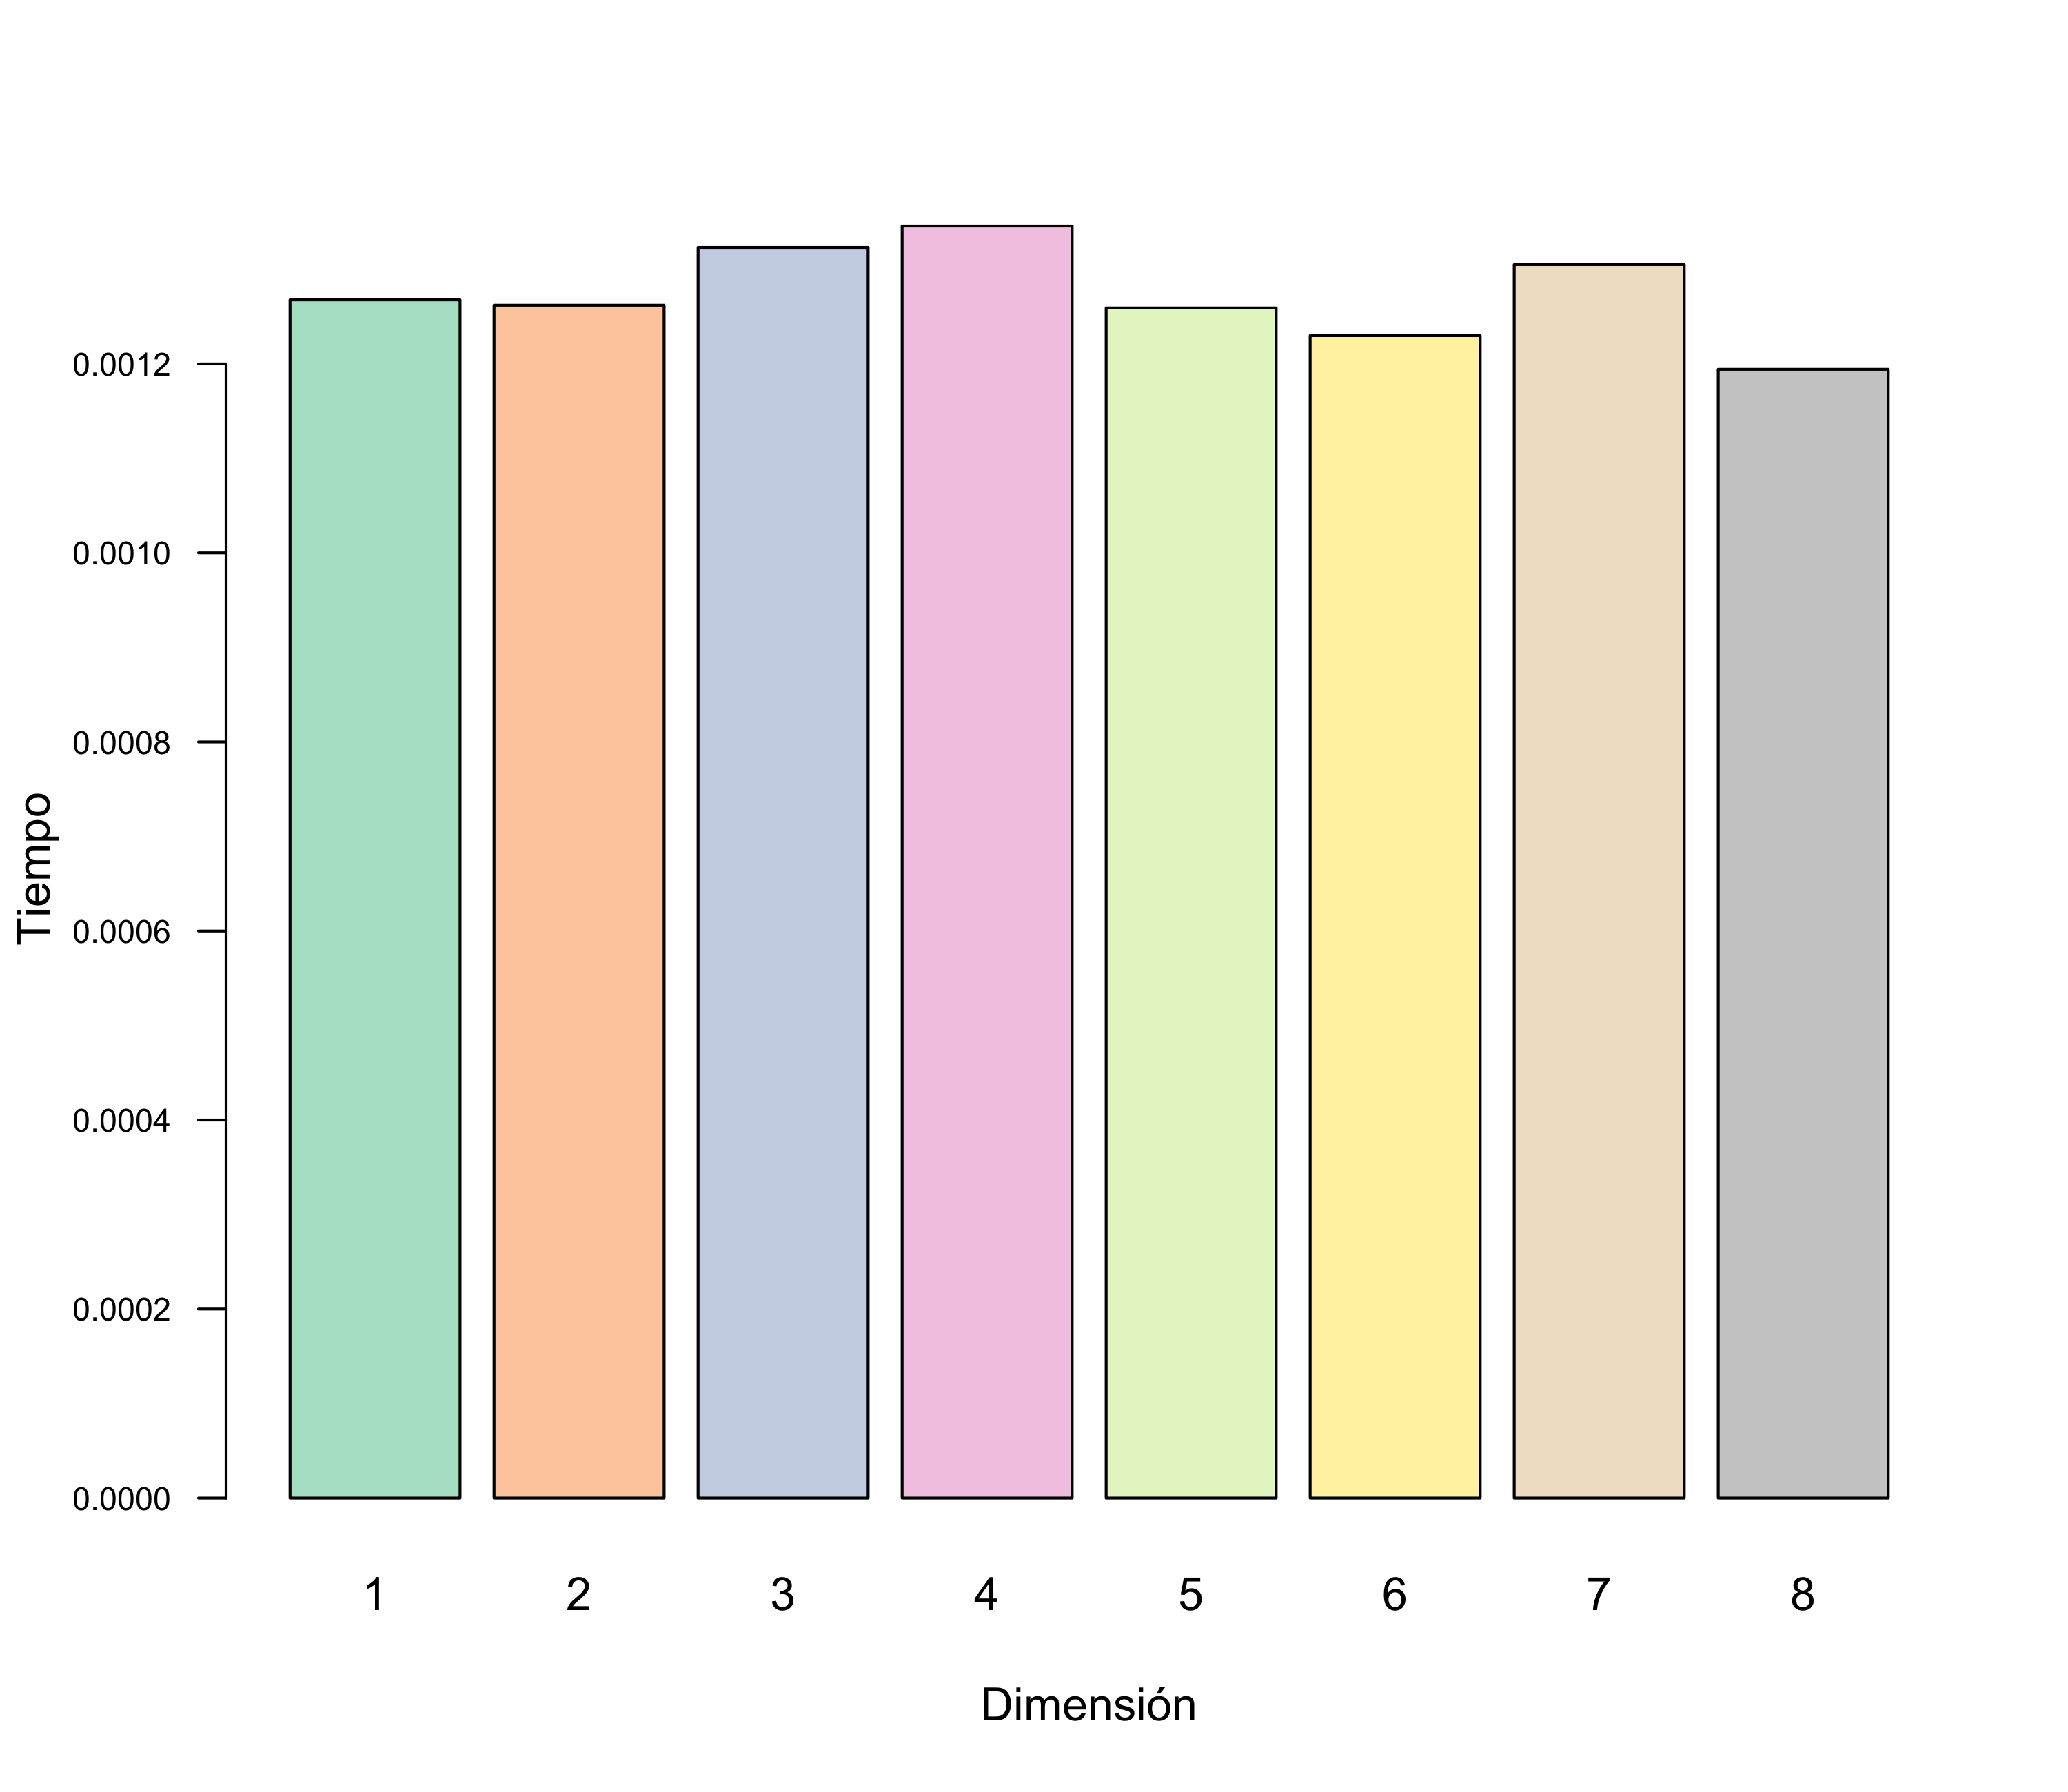
\includegraphics[width=\linewidth]{128-tiempo.png}
 		\caption{Caminata de 128 pasos.}
 		\label{128tiempo}
 	\end{subfigure}
	\begin{subfigure}[b]{0.45\linewidth}
 		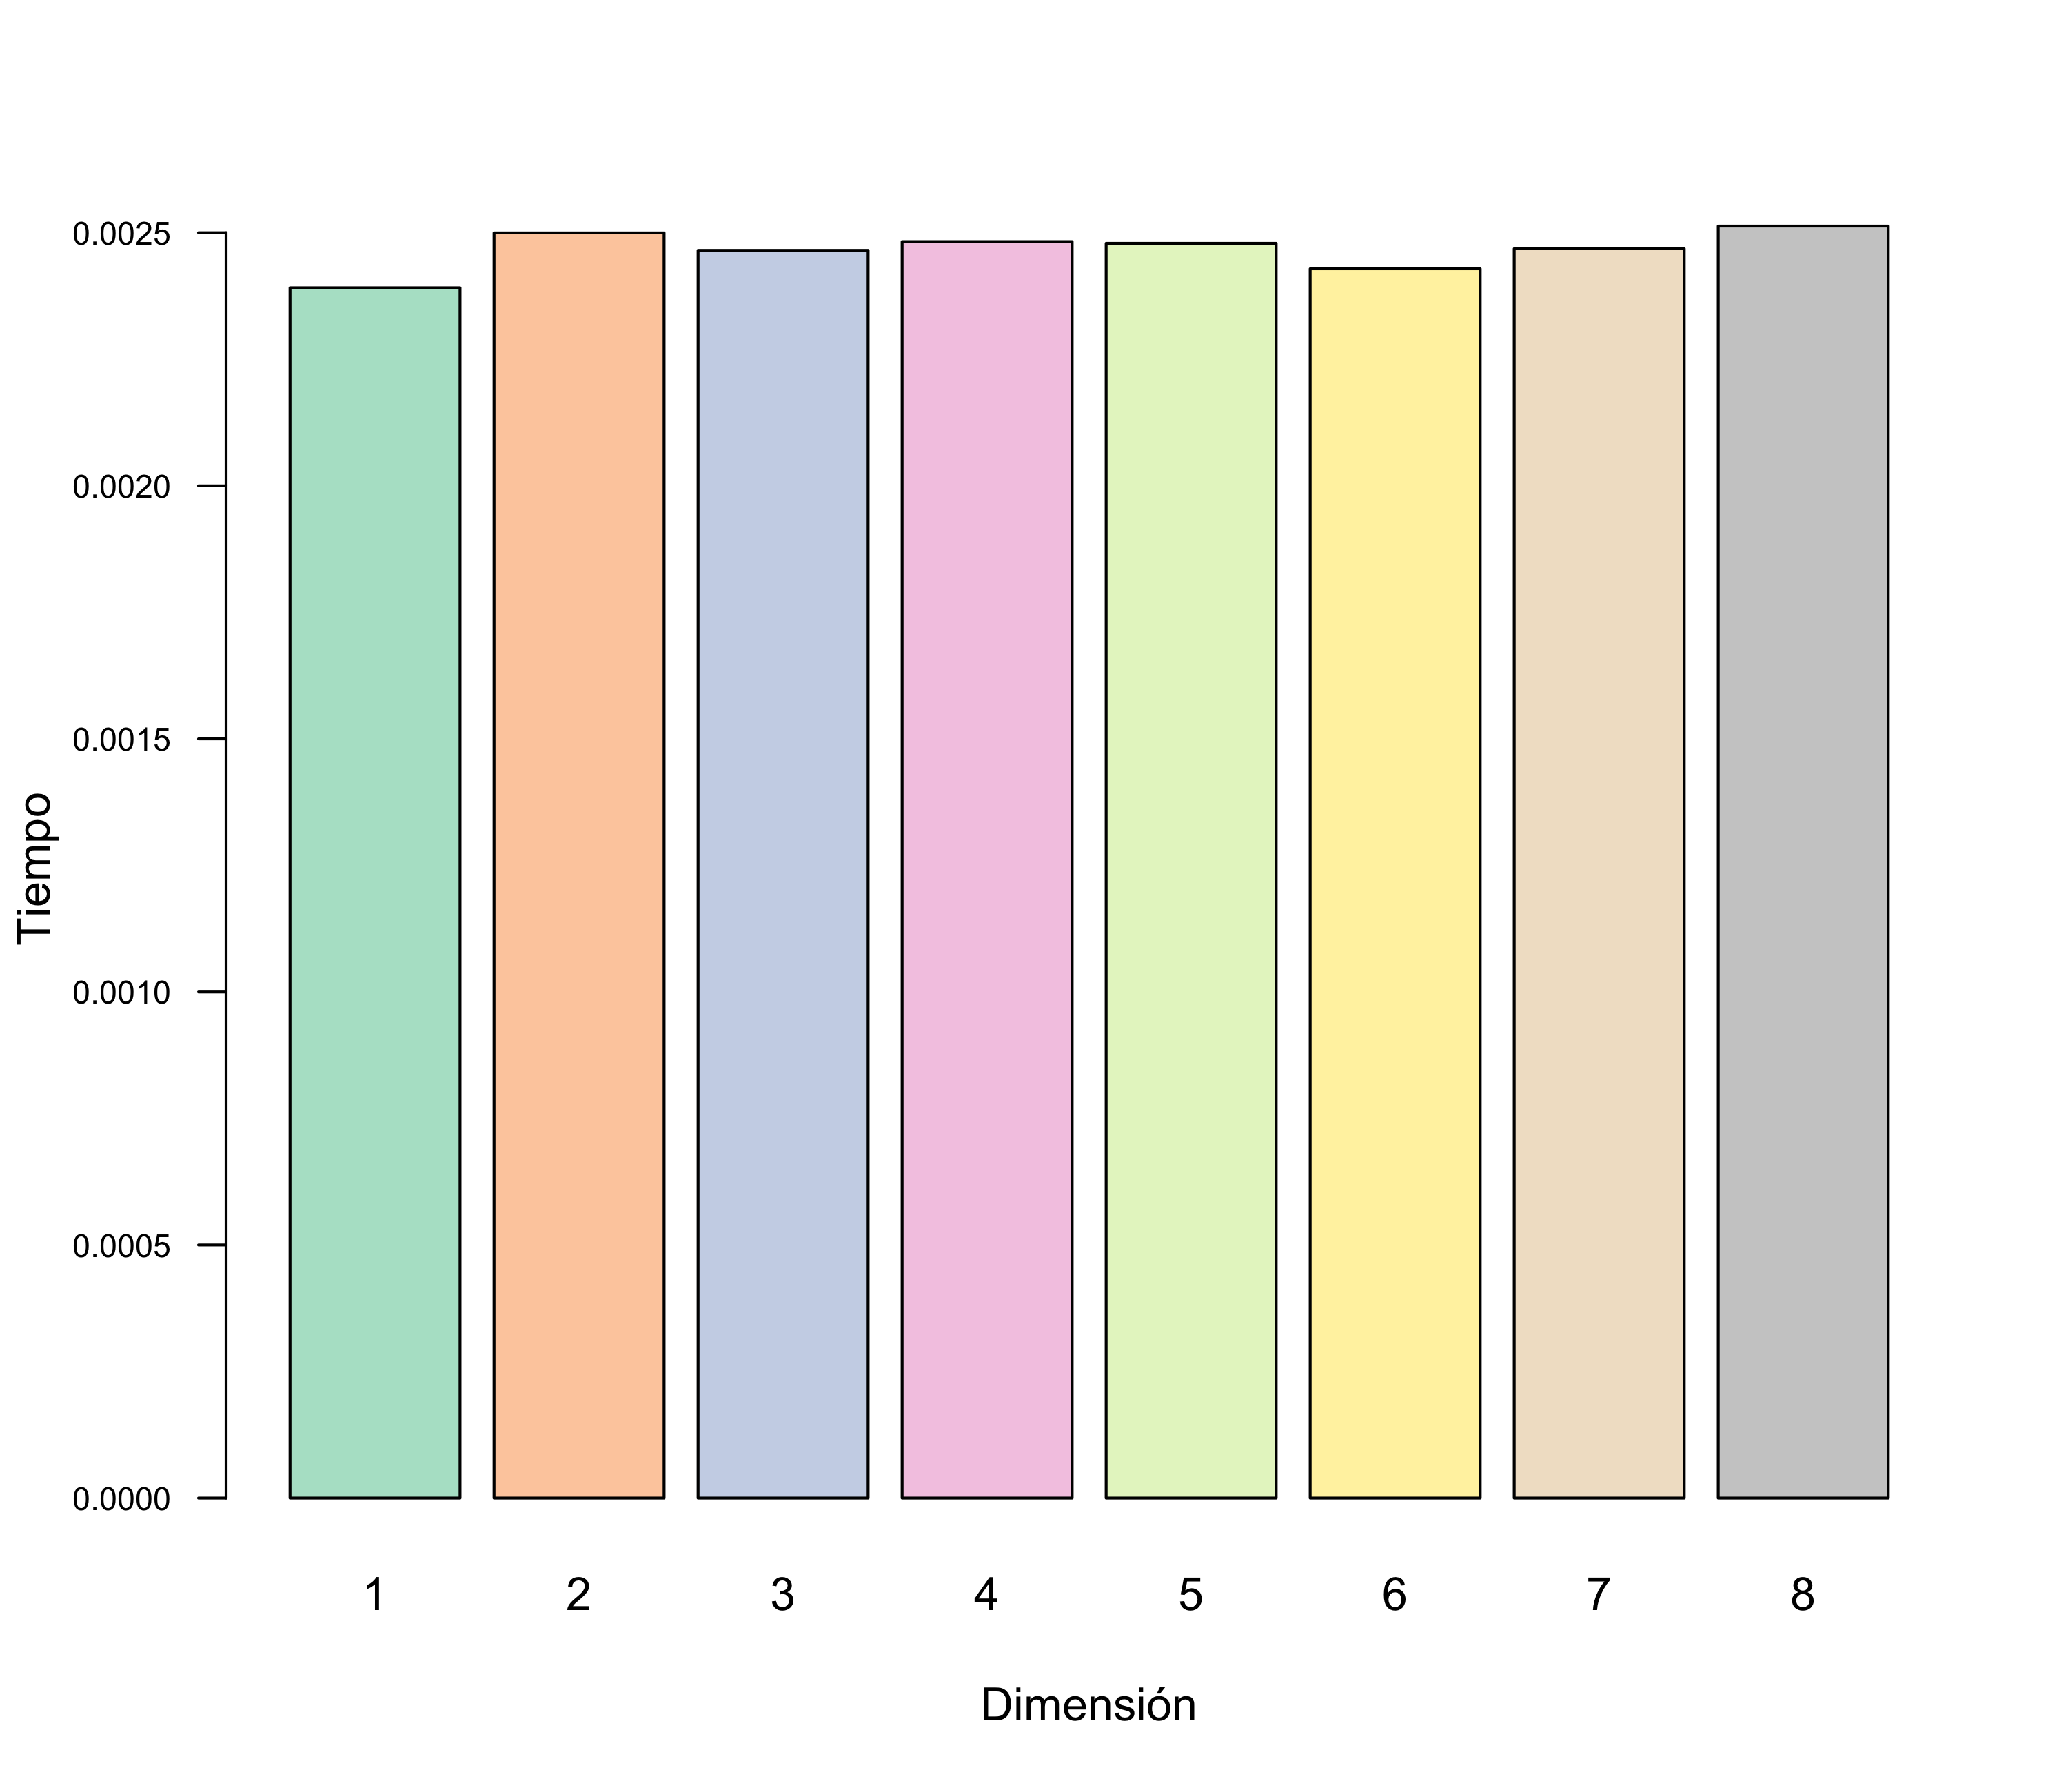
\includegraphics[width=\linewidth]{256-tiempo.png}
 		 \caption{Caminata de 256 pasos.}
 		\label{256tiempo}
 	\end{subfigure}
 		\begin{subfigure}[b]{0.45\linewidth}
 		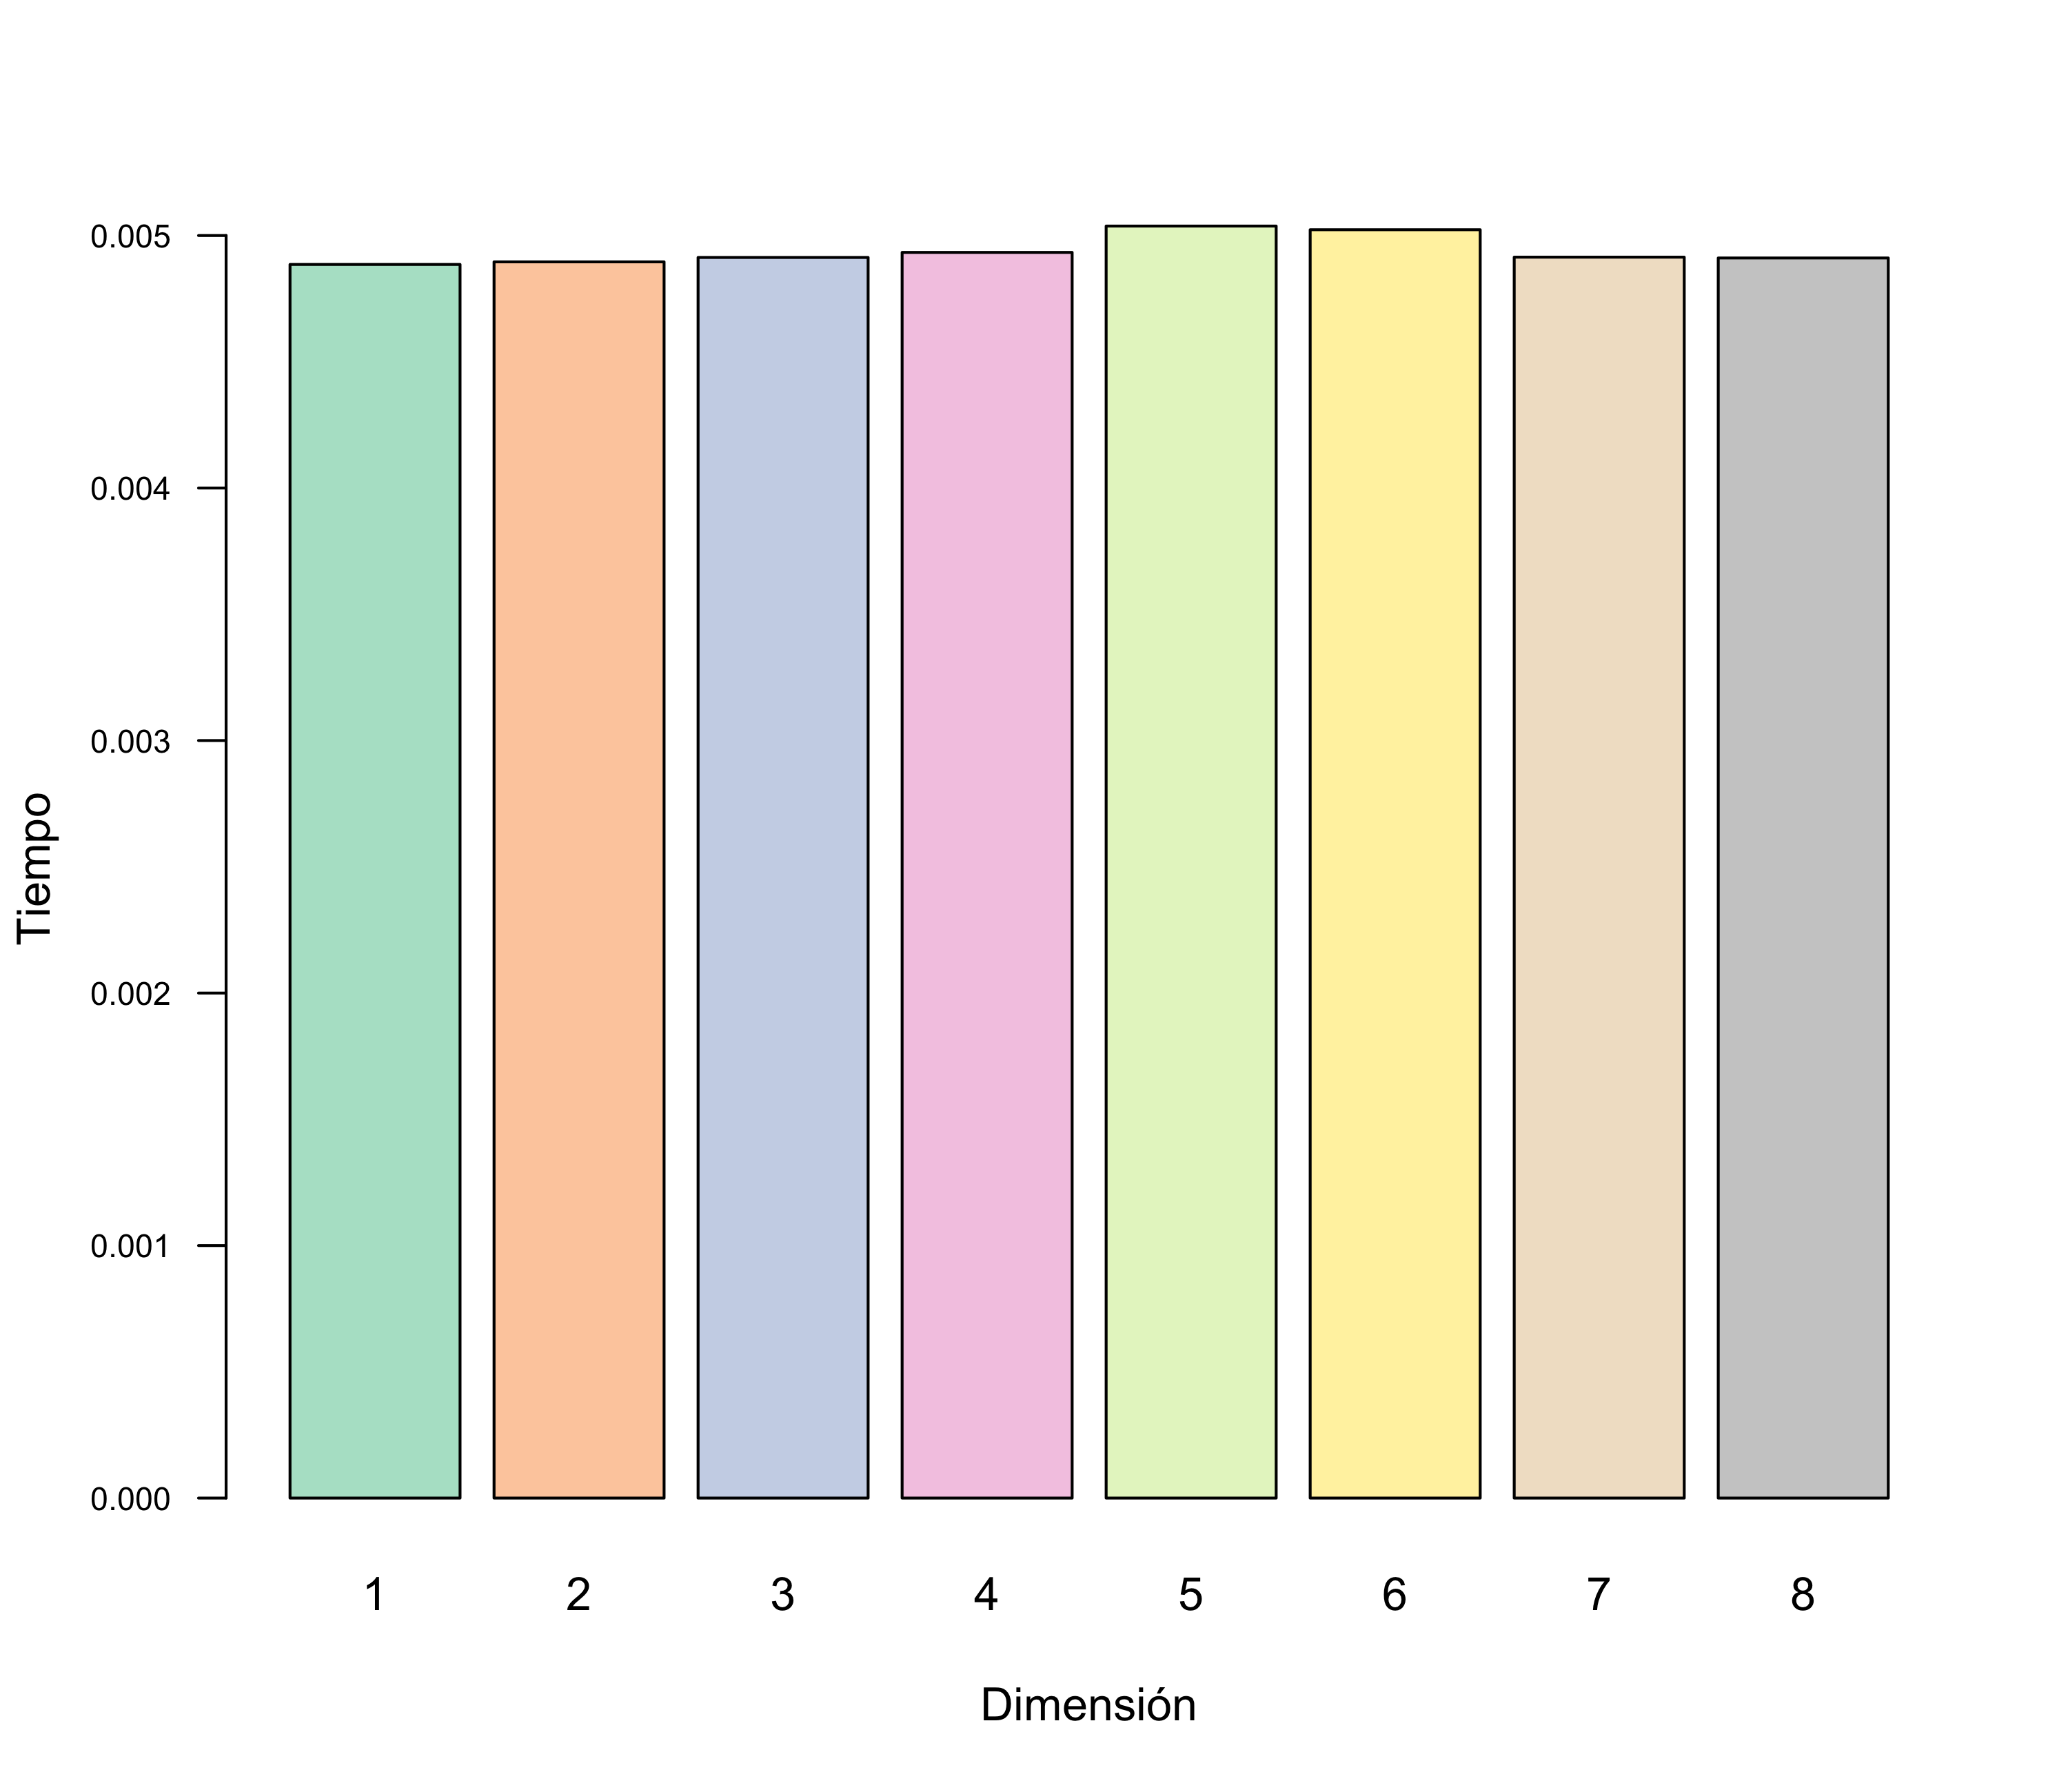
\includegraphics[width=\linewidth]{512-tiempo.png}
 		 \caption{Caminata de 512 pasos.}
 		\label{512tiempo}
 	\end{subfigure}
 		\begin{subfigure}[b]{0.45\linewidth}
 		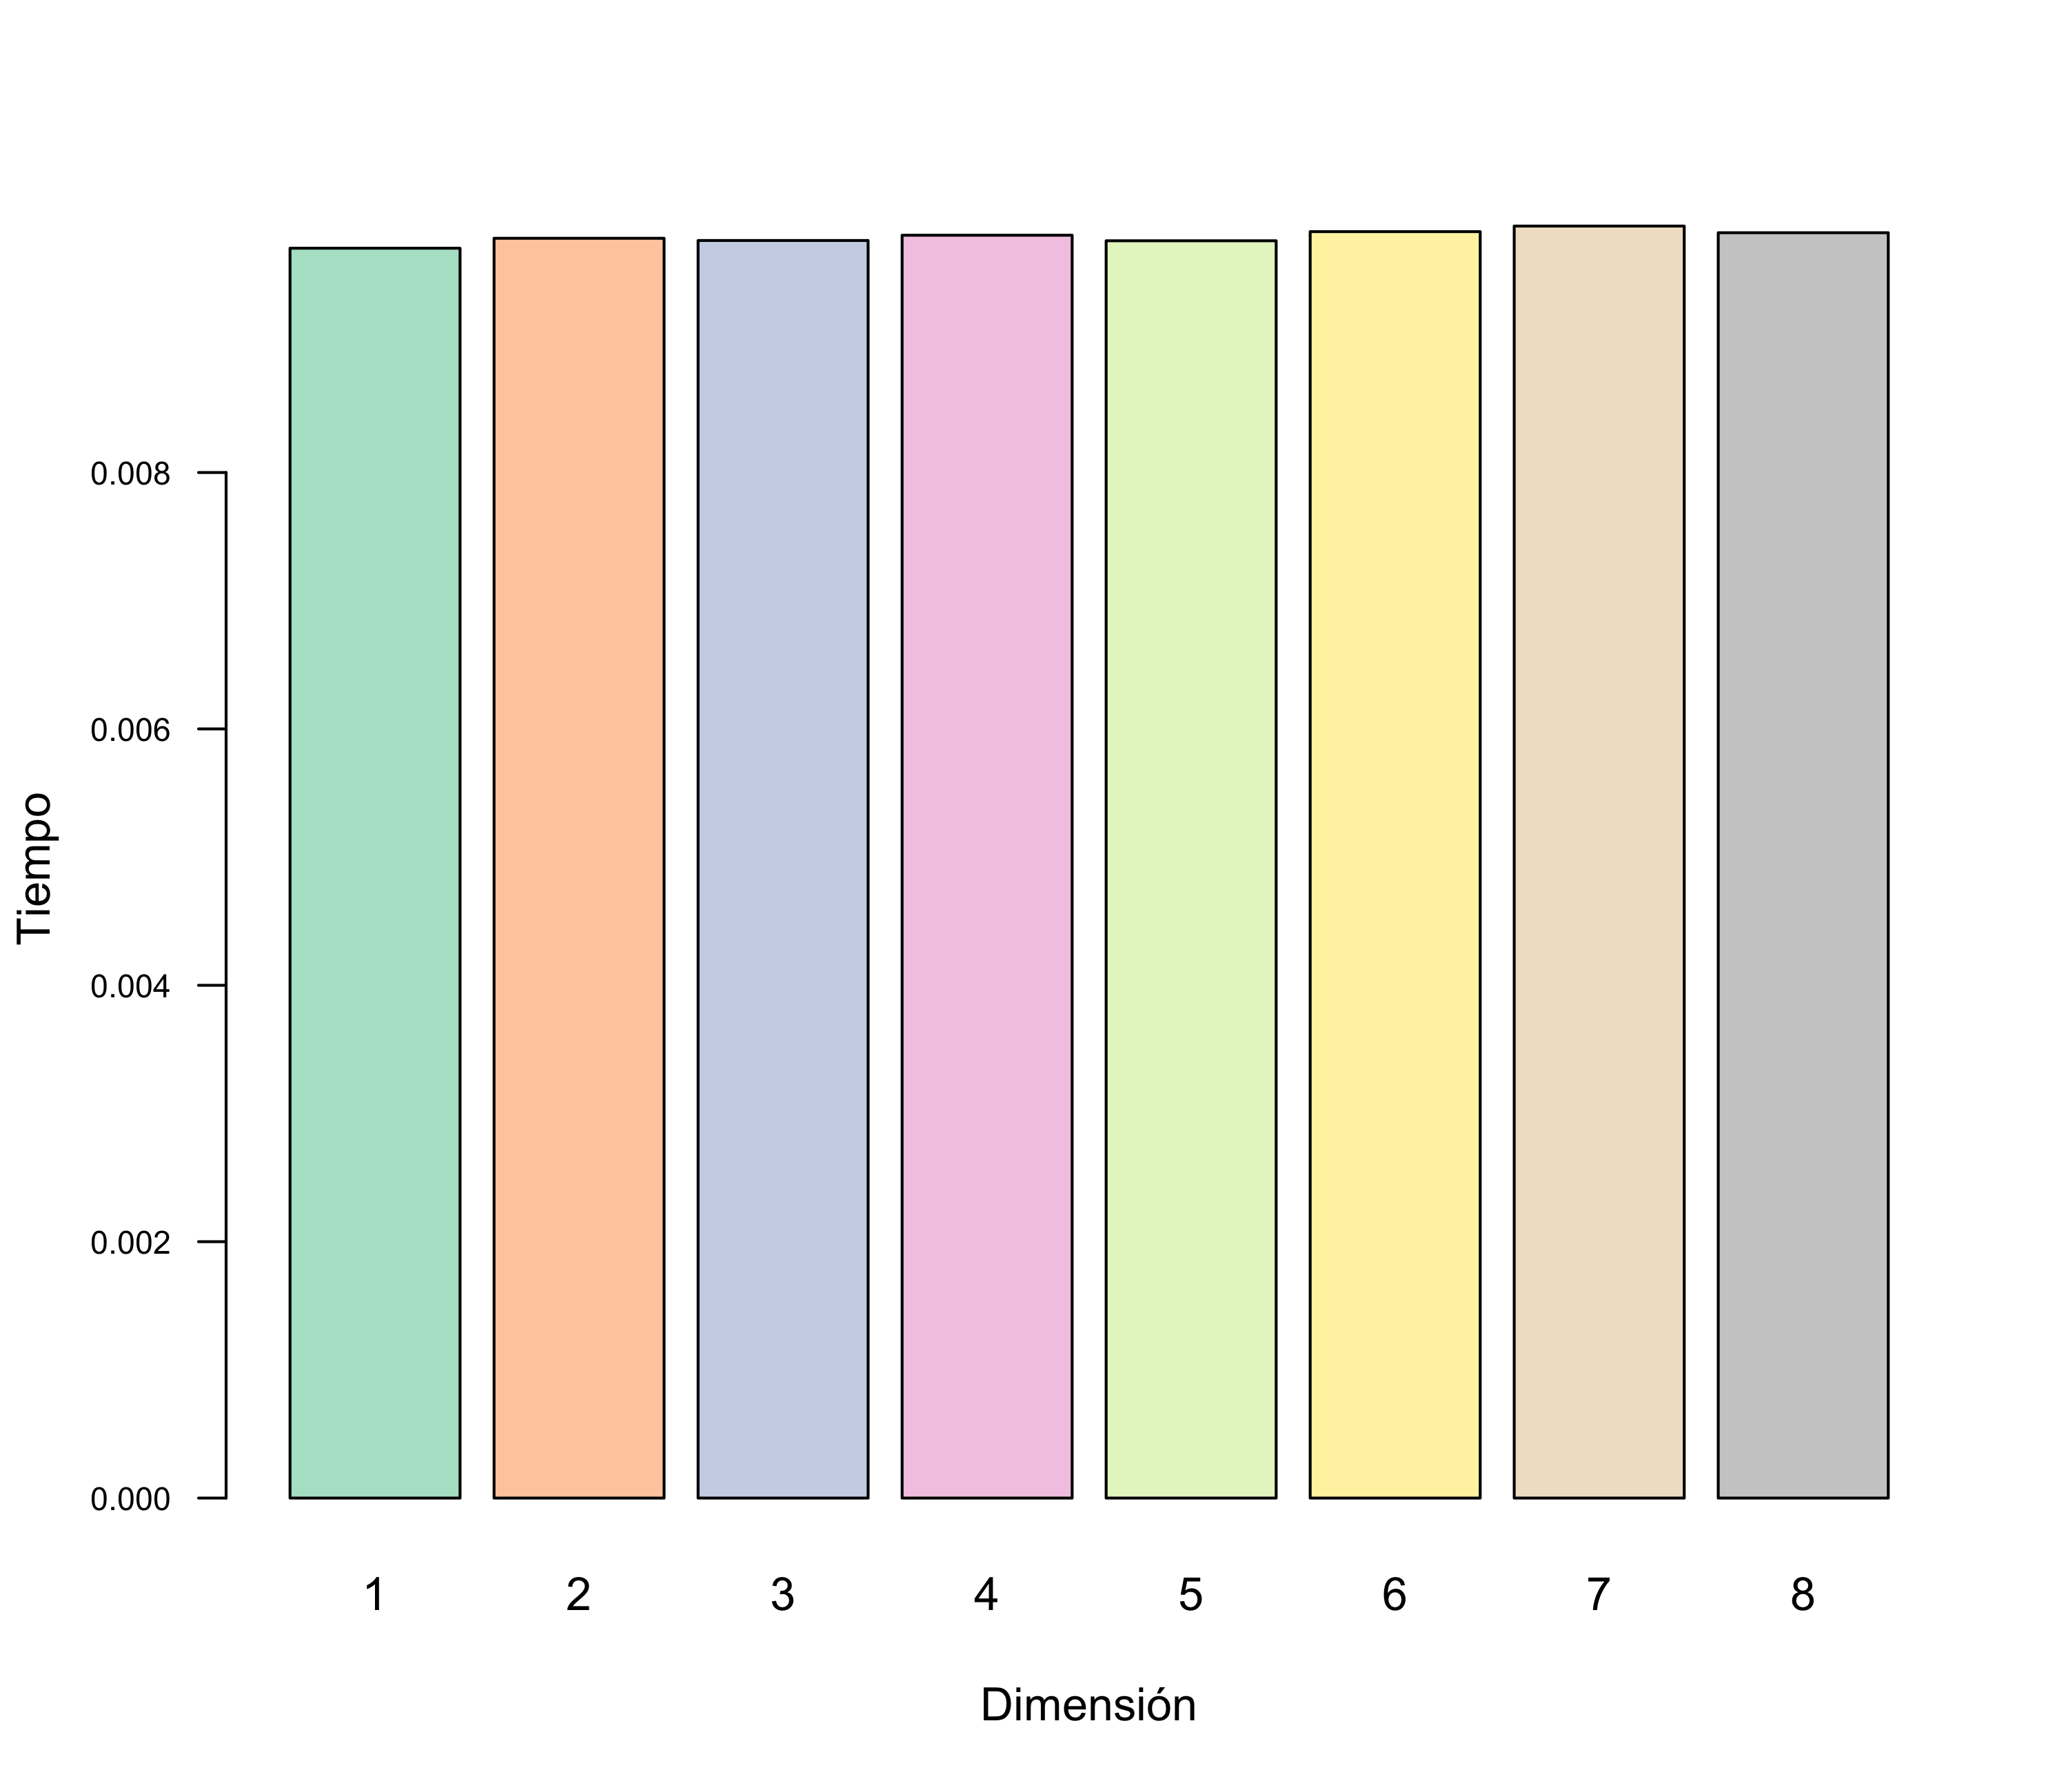
\includegraphics[width=\linewidth]{1024-tiempo.png}
 		\caption{Caminata de 1024 pasos.}
 		\label{1024tiempo}
 		\end{subfigure}
 		 	\caption{Tiempos dependiendo de la dimensión, variando la longitud de la caminata.} 
\label{tiempo-largos}
 \end{figure}
 
\begin{figure}
 	 \centering
 	 \begin{subfigure}[b]{0.3\linewidth}
 		 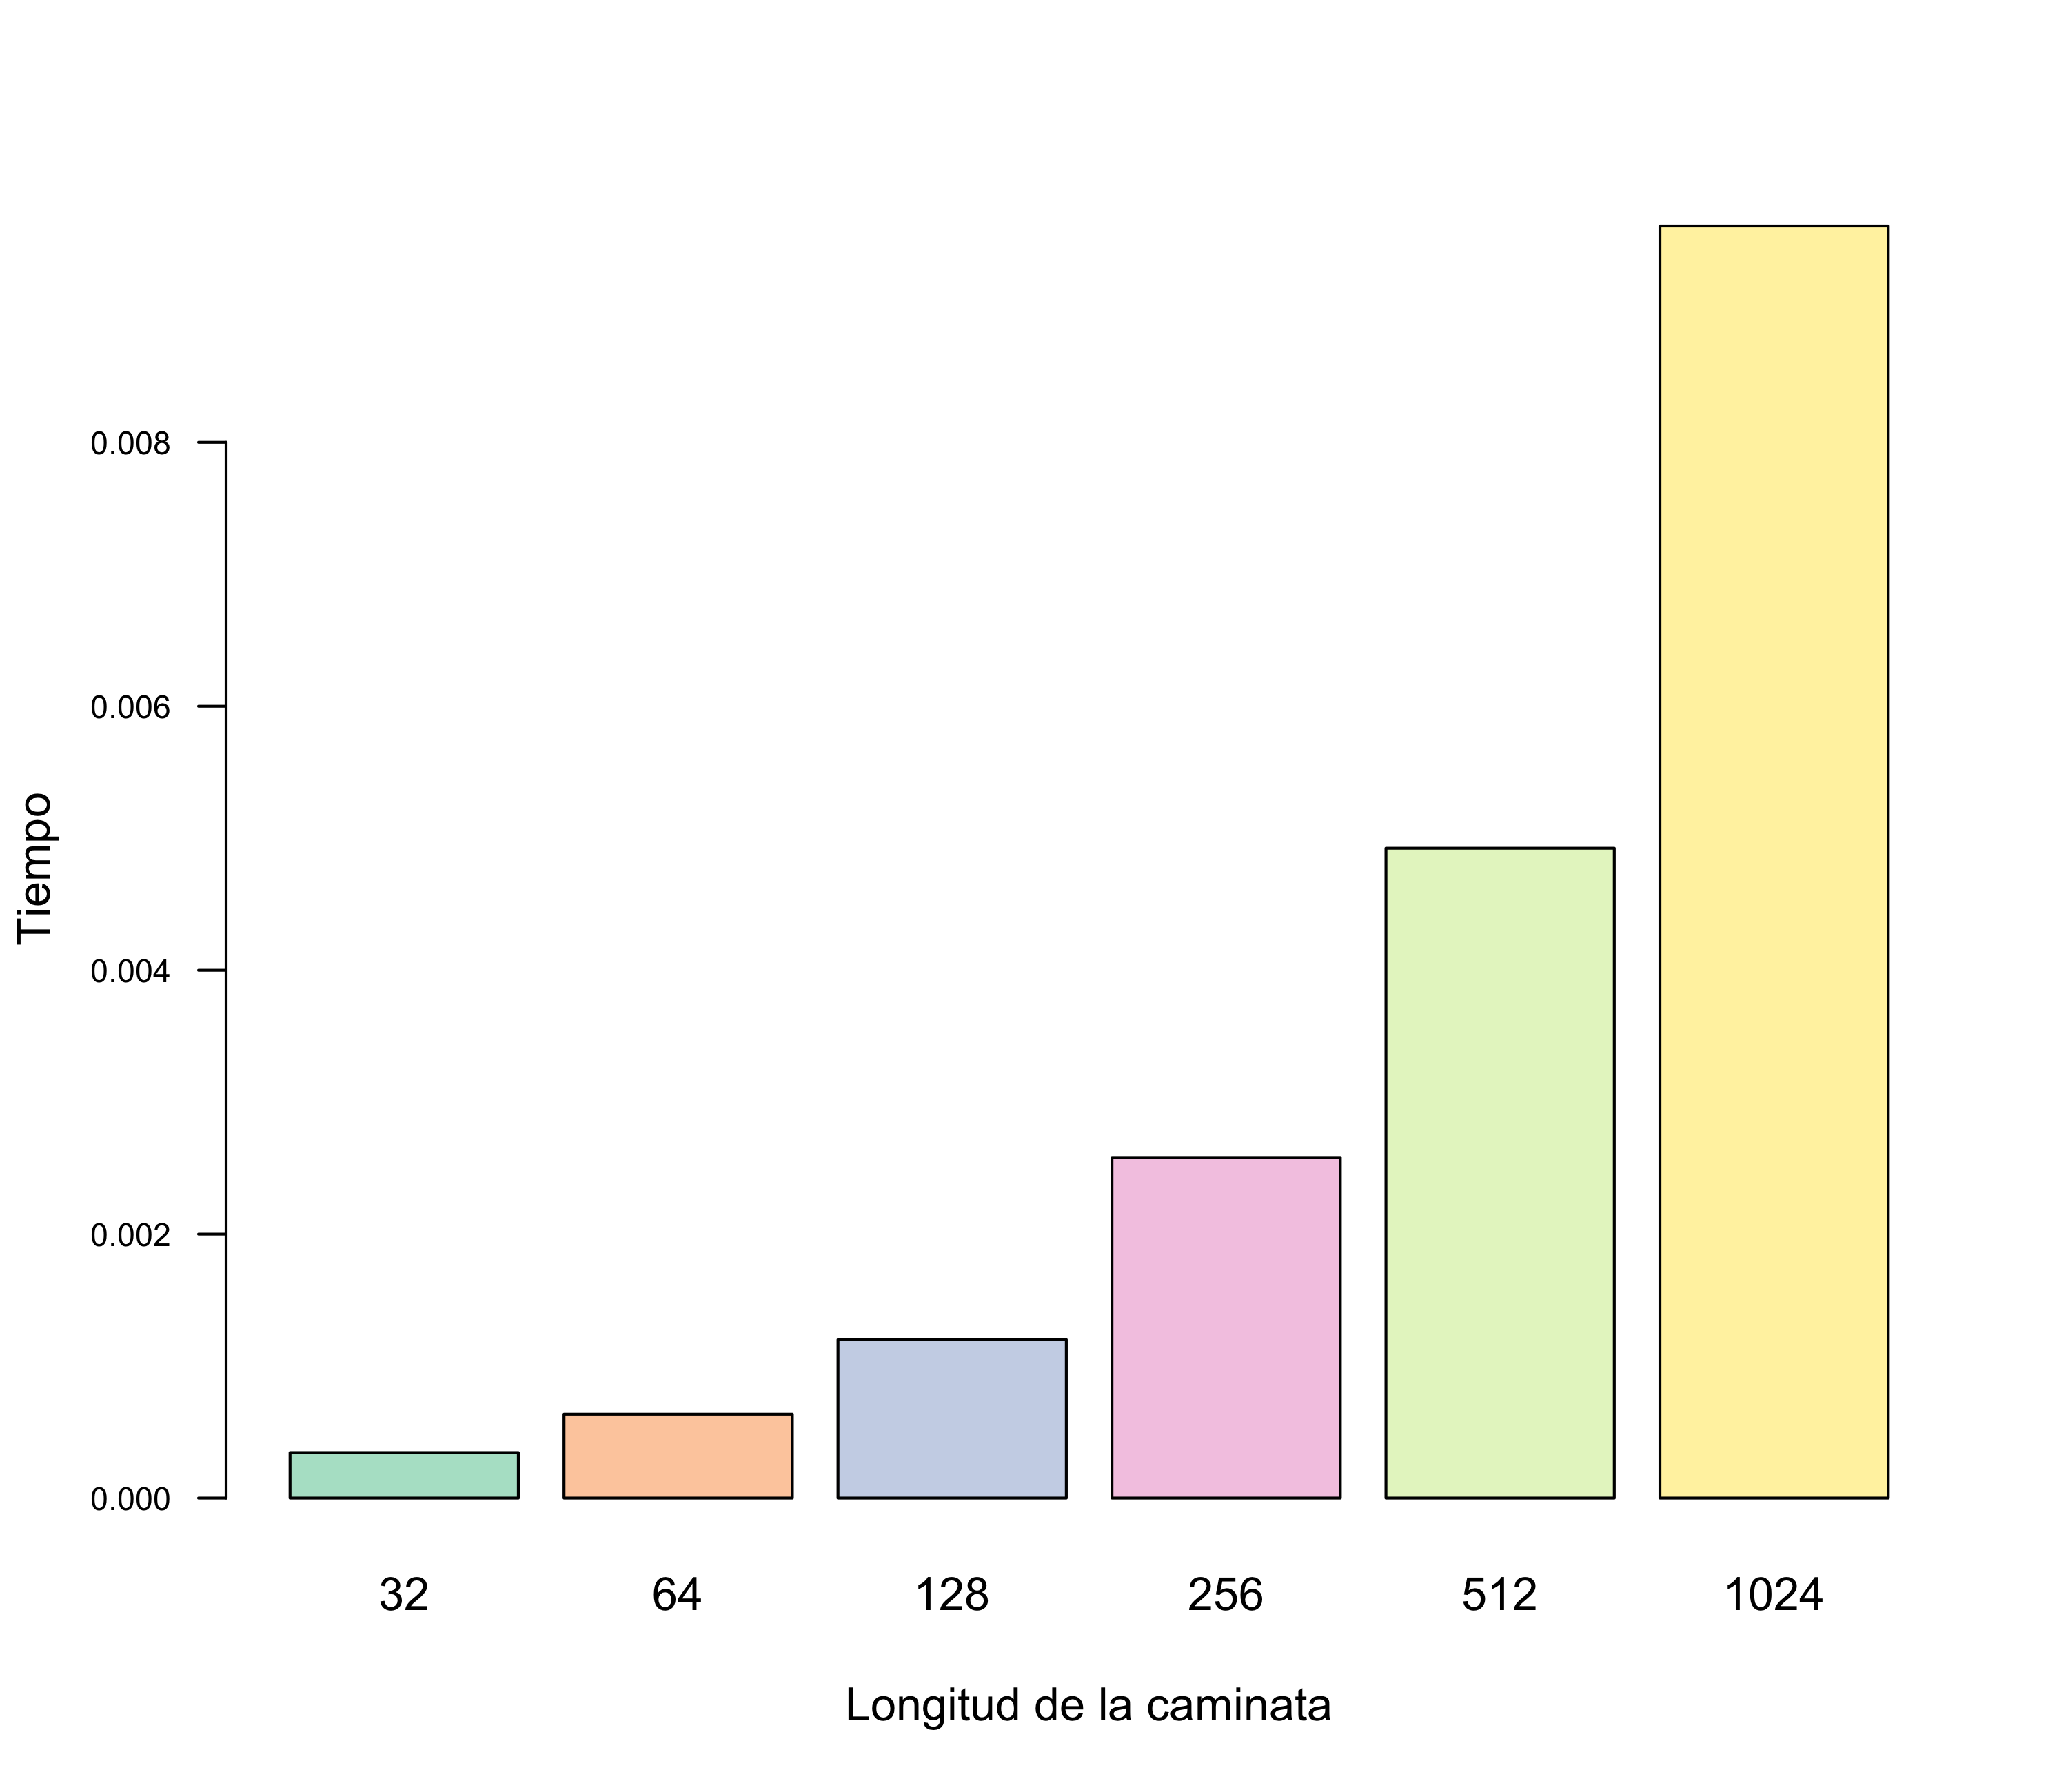
\includegraphics[width=\linewidth]{dimension1-tiempo.png} 		
 		 \caption{Dimensión 1.}
 		 	 	\label{tiempos-dim1}
 	 \end{subfigure}
 	 \begin{subfigure}[b]{0.3\linewidth}

 		 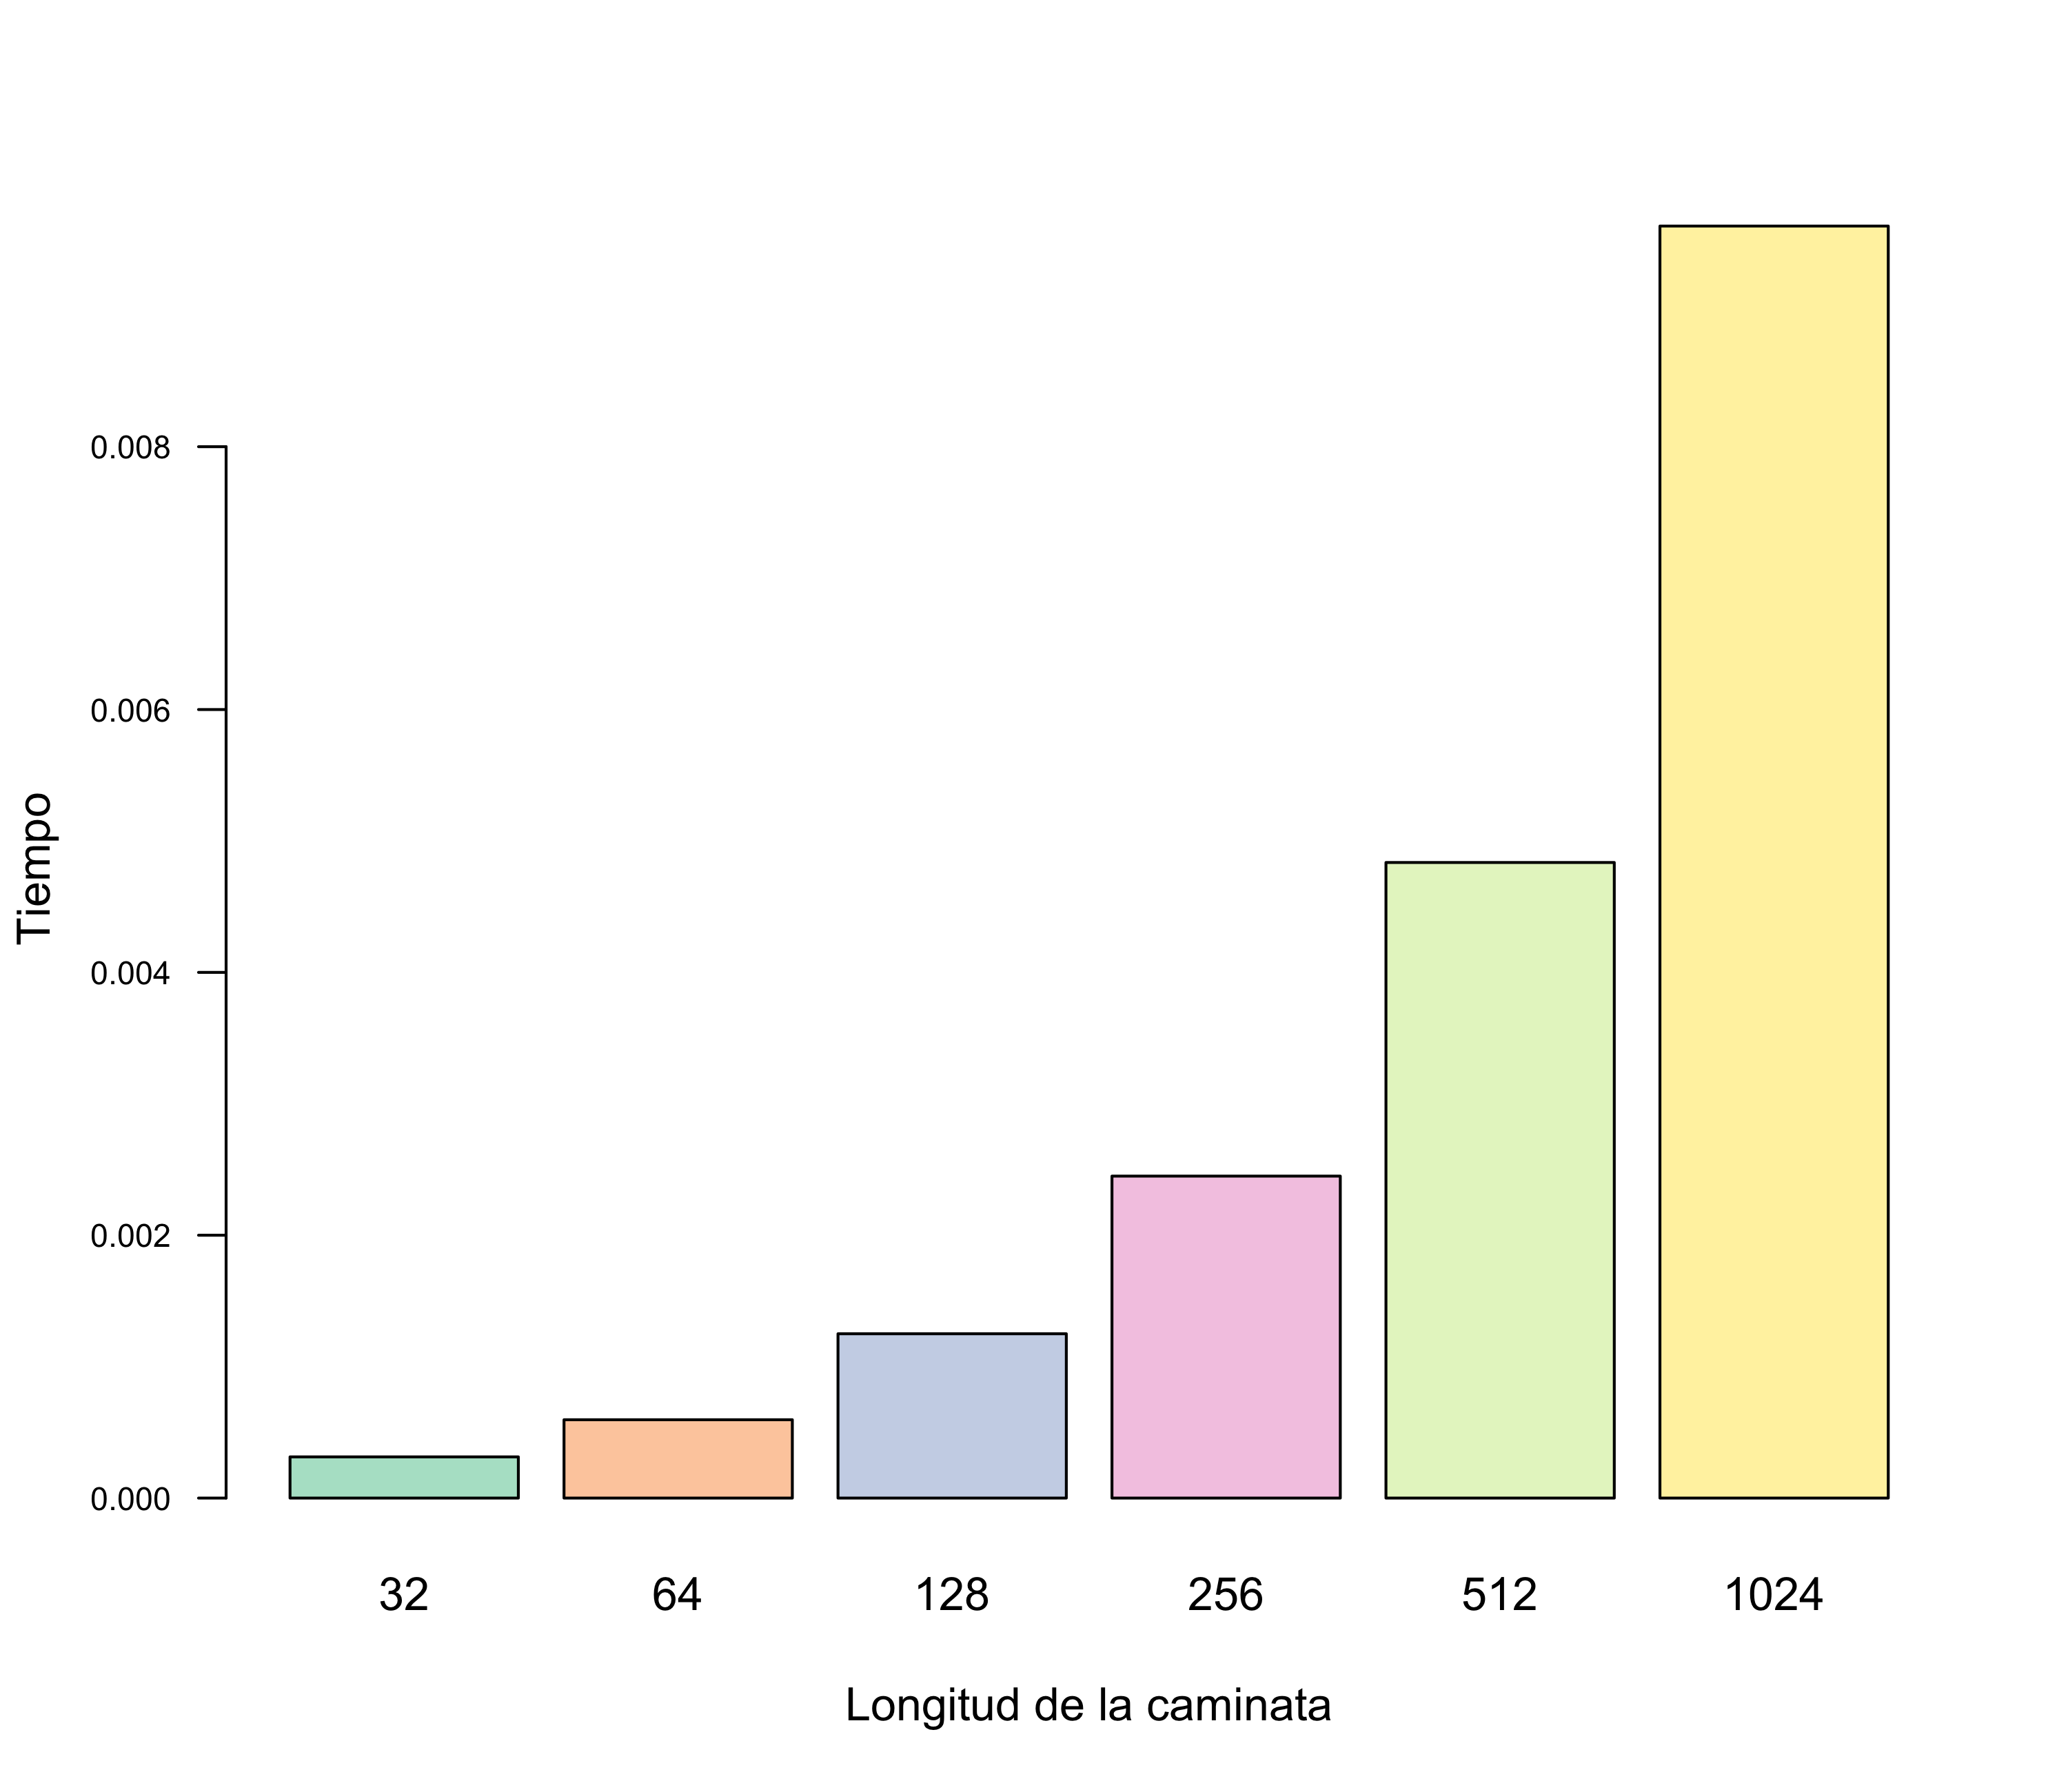
\includegraphics[width=\linewidth]{dimension2-tiempo.png} 		
 		 \caption{Dimensión 2.}
 		 \label{tiempos-dim2}
 	 \end{subfigure}
  	\begin{subfigure}[b]{0.3\linewidth}
 		 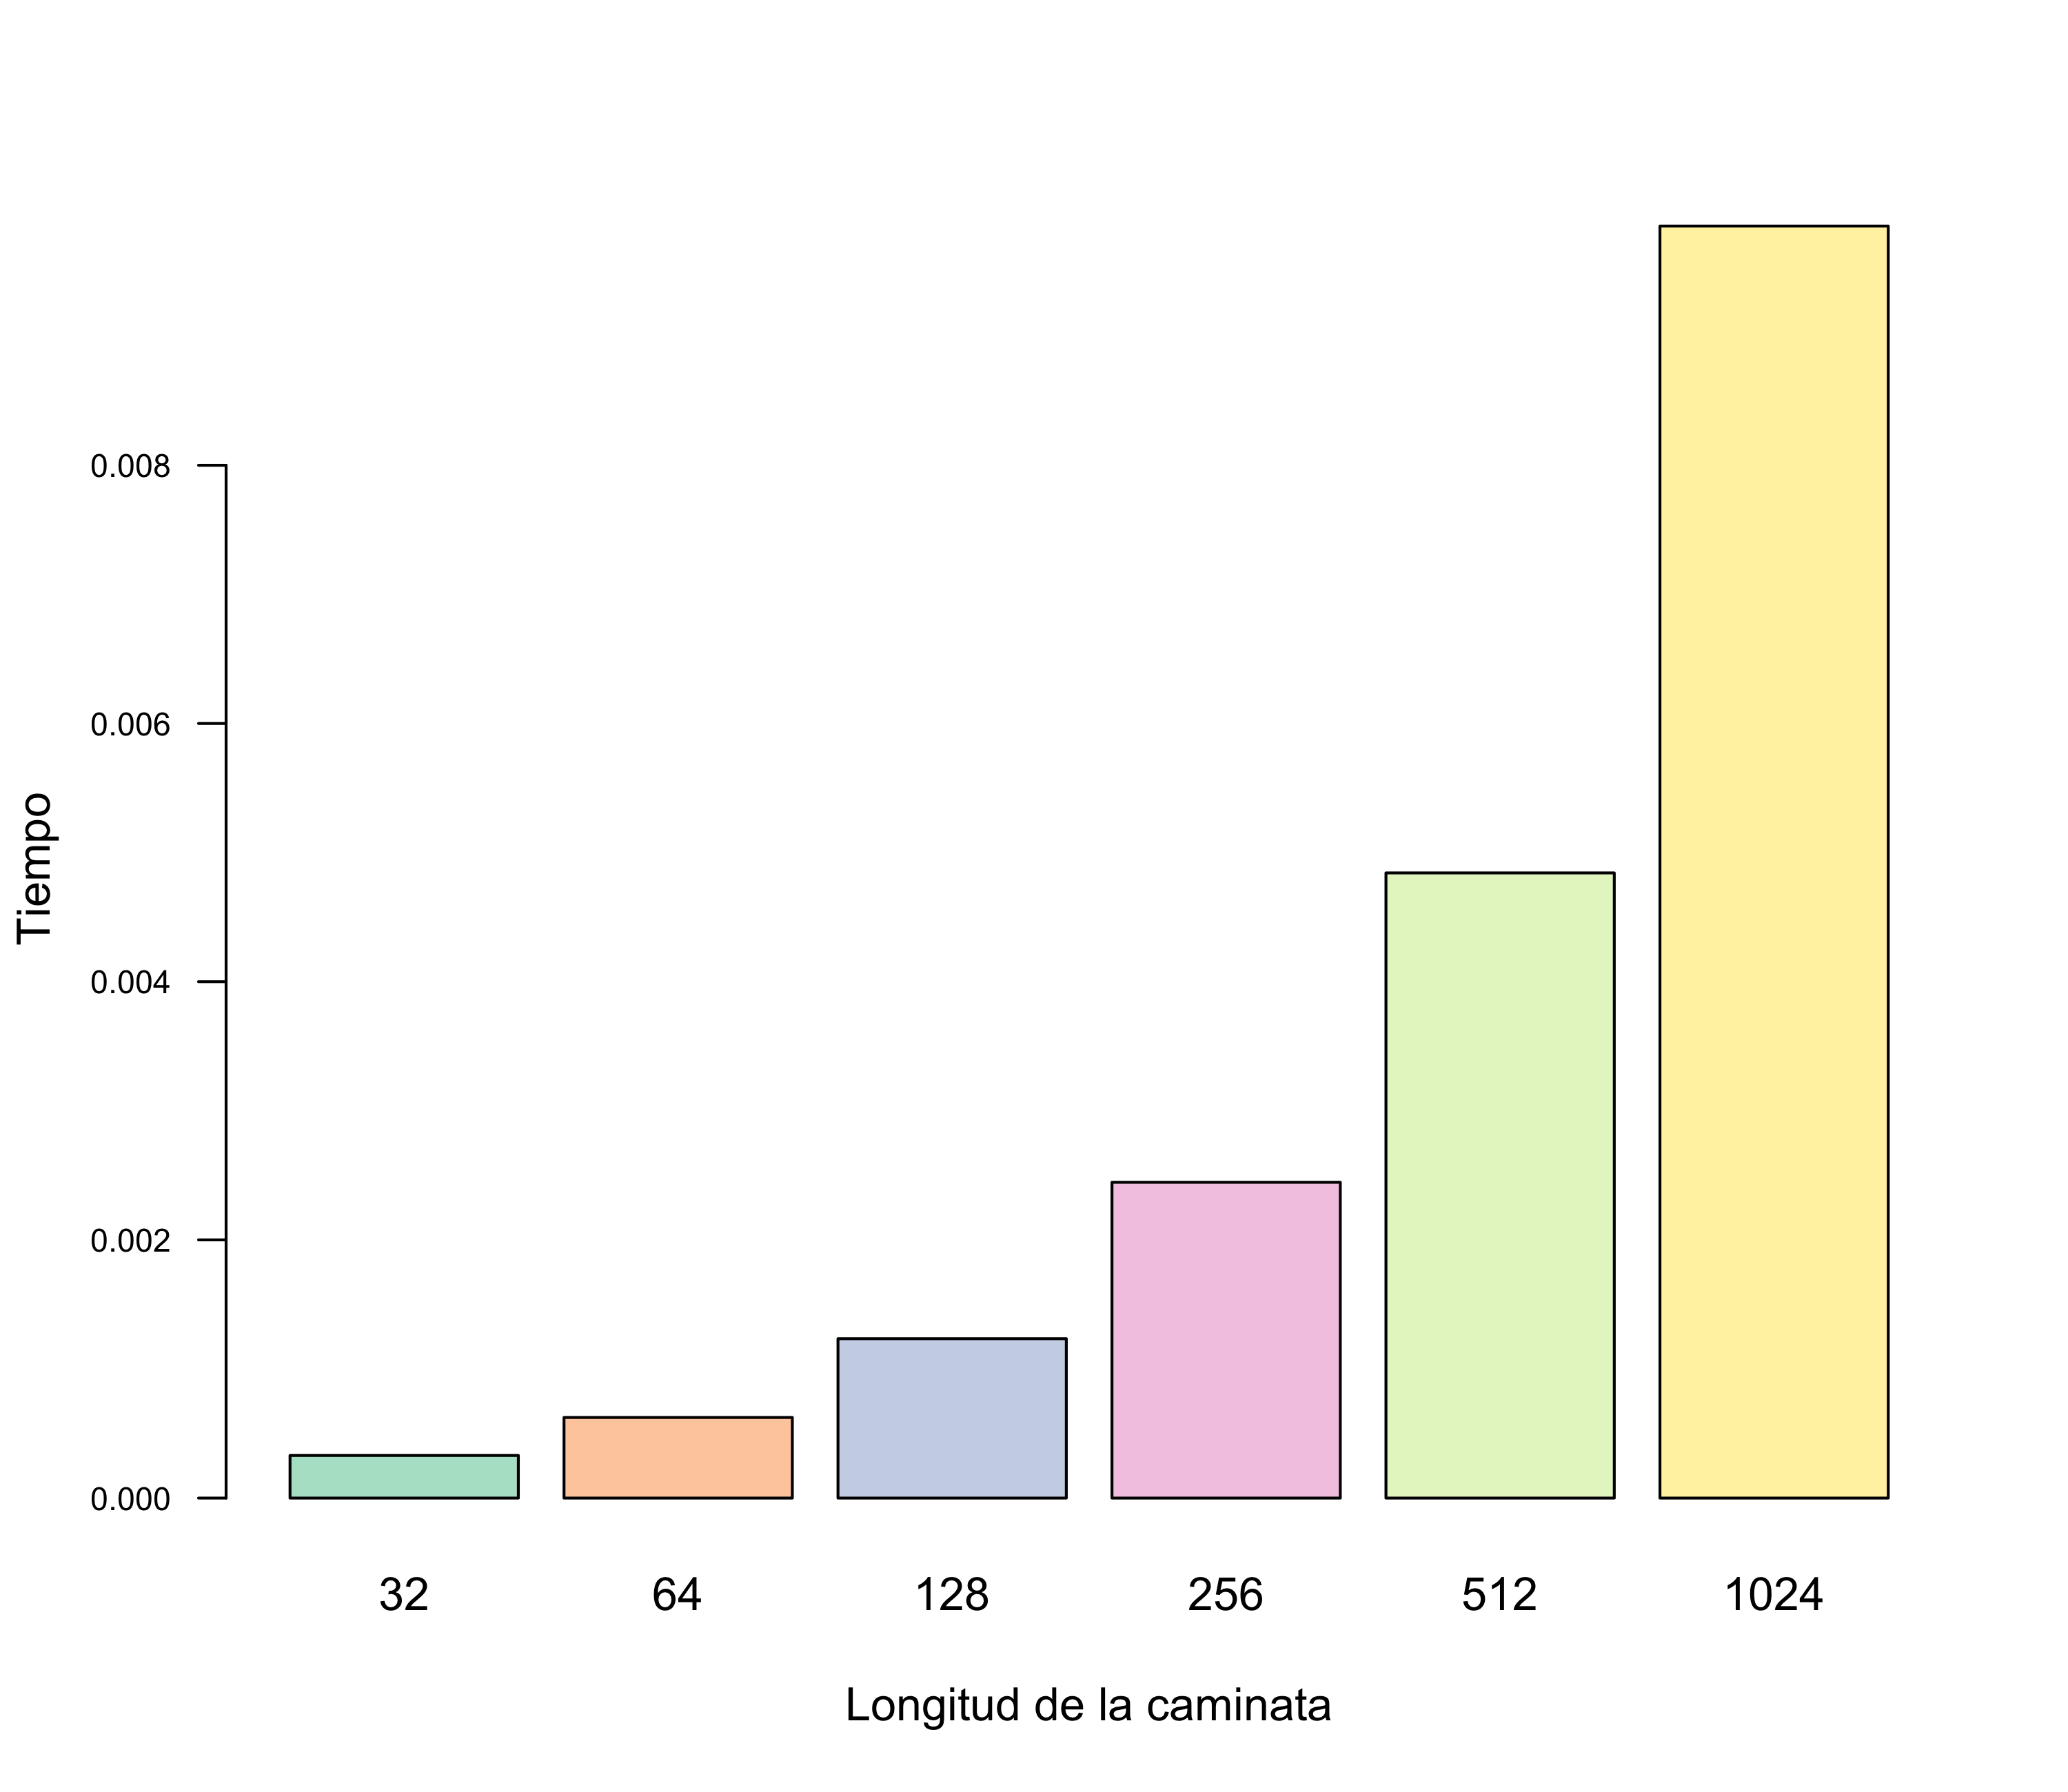
\includegraphics[width=\linewidth]{dimension3-tiempo.png}
 	 	\caption{Dimensión 3.}
 	 	\label{tiempos-dim3}
  	\end{subfigure}
 	\begin{subfigure}[b]{0.3\linewidth} 		
  		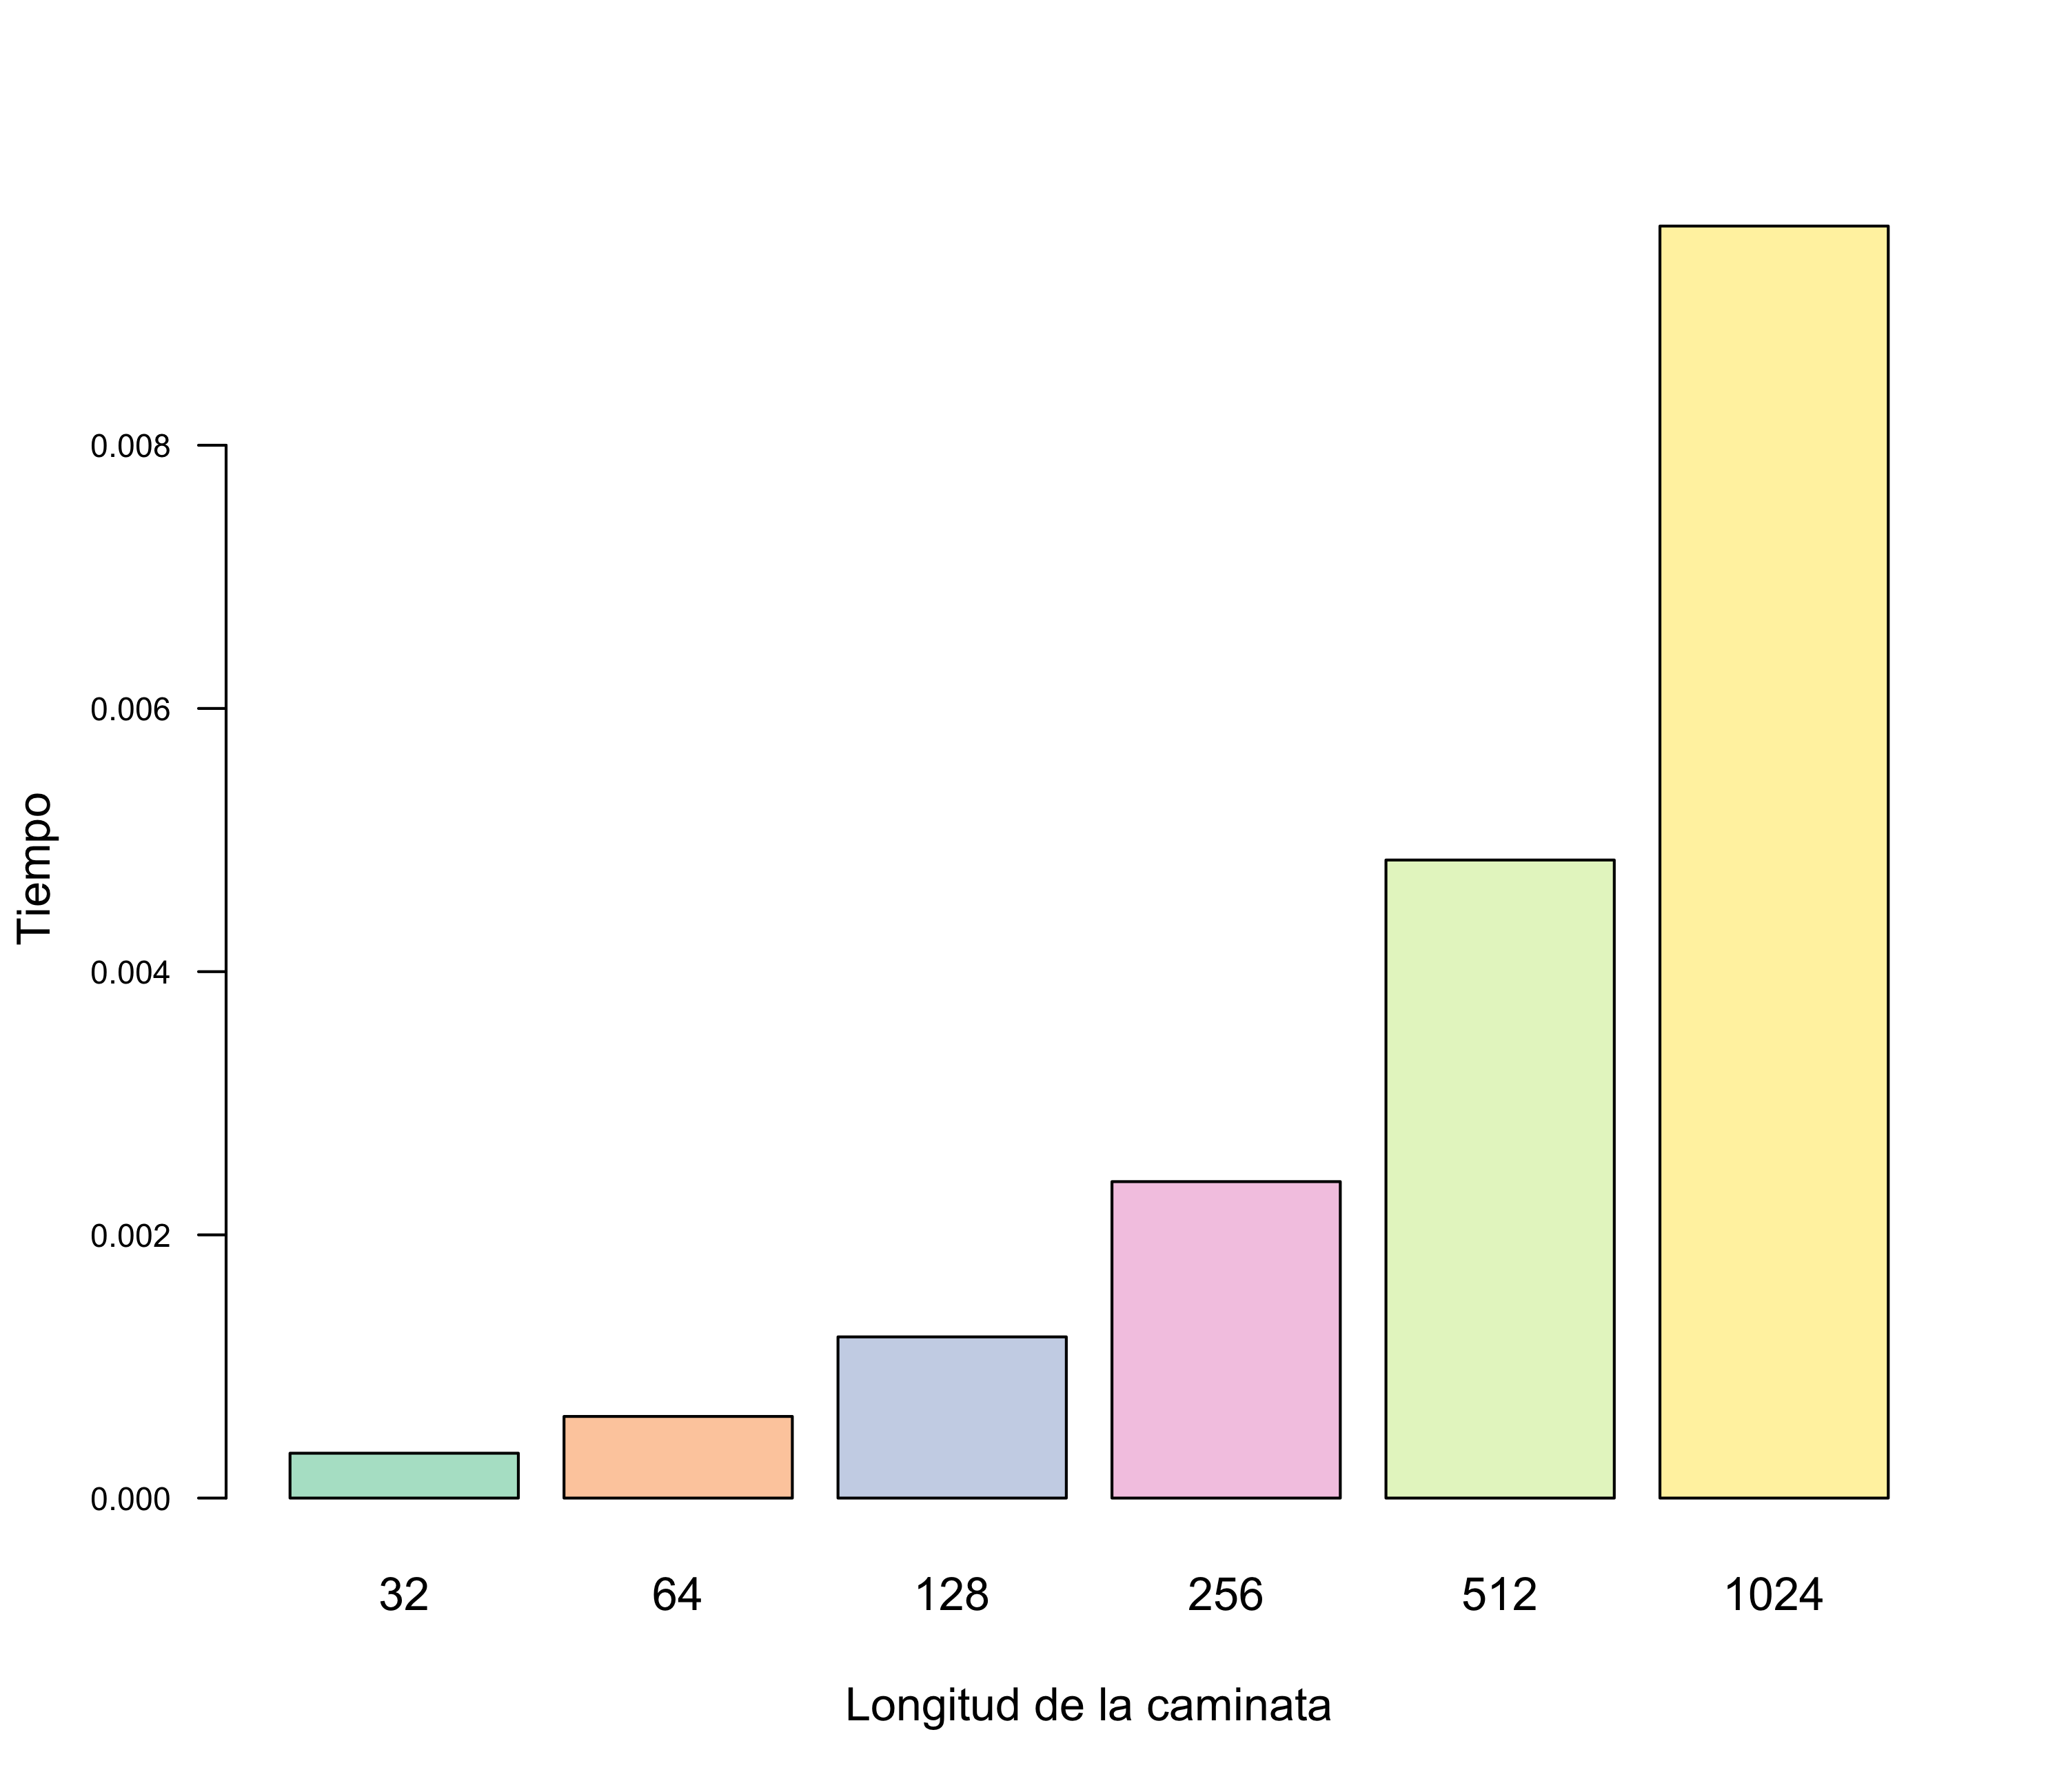
\includegraphics[width=\linewidth]{dimension4-tiempo.png}
  		\caption{Dimensión 4.}
  		\label{tiempos-dim4}
  	\end{subfigure}
  		\begin{subfigure}[b]{0.3\linewidth}
  		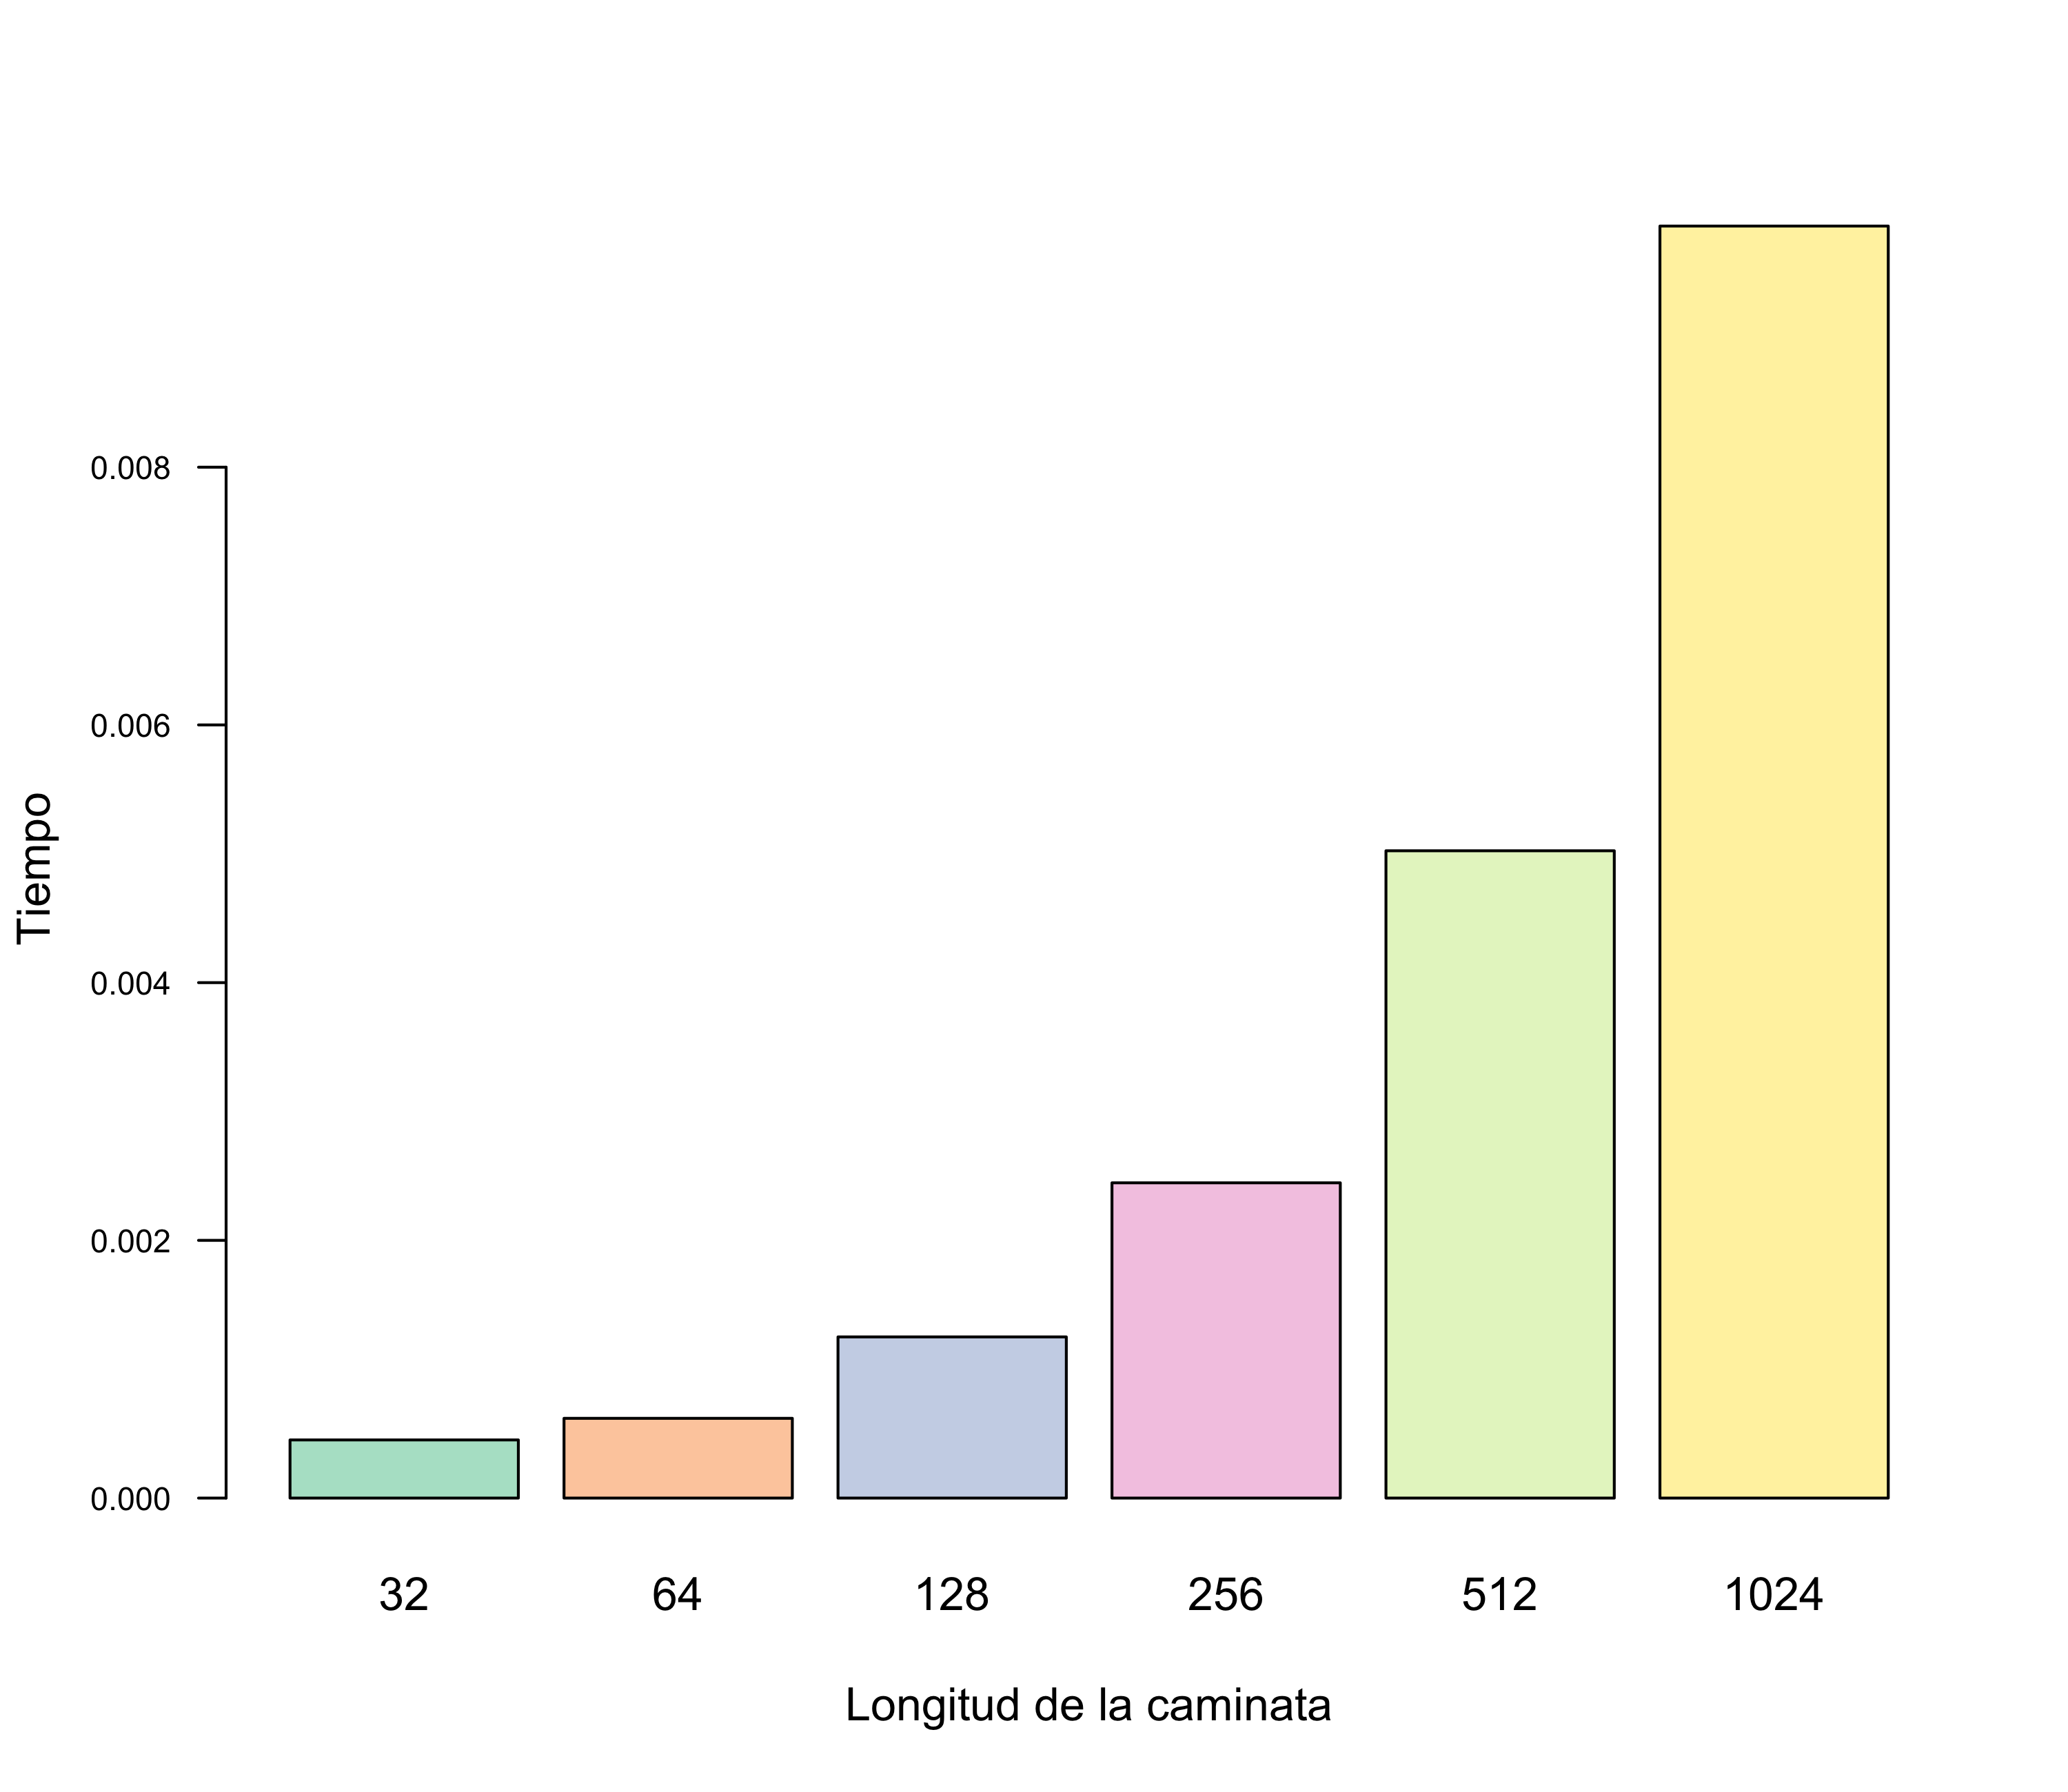
\includegraphics[width=\linewidth]{dimension5-tiempo.png} 		
  		\caption{Dimensión 5.}
  		\label{tiempos-dim5}
  	\end{subfigure}
 	 	\begin{subfigure}[b]{0.3\linewidth}
 		 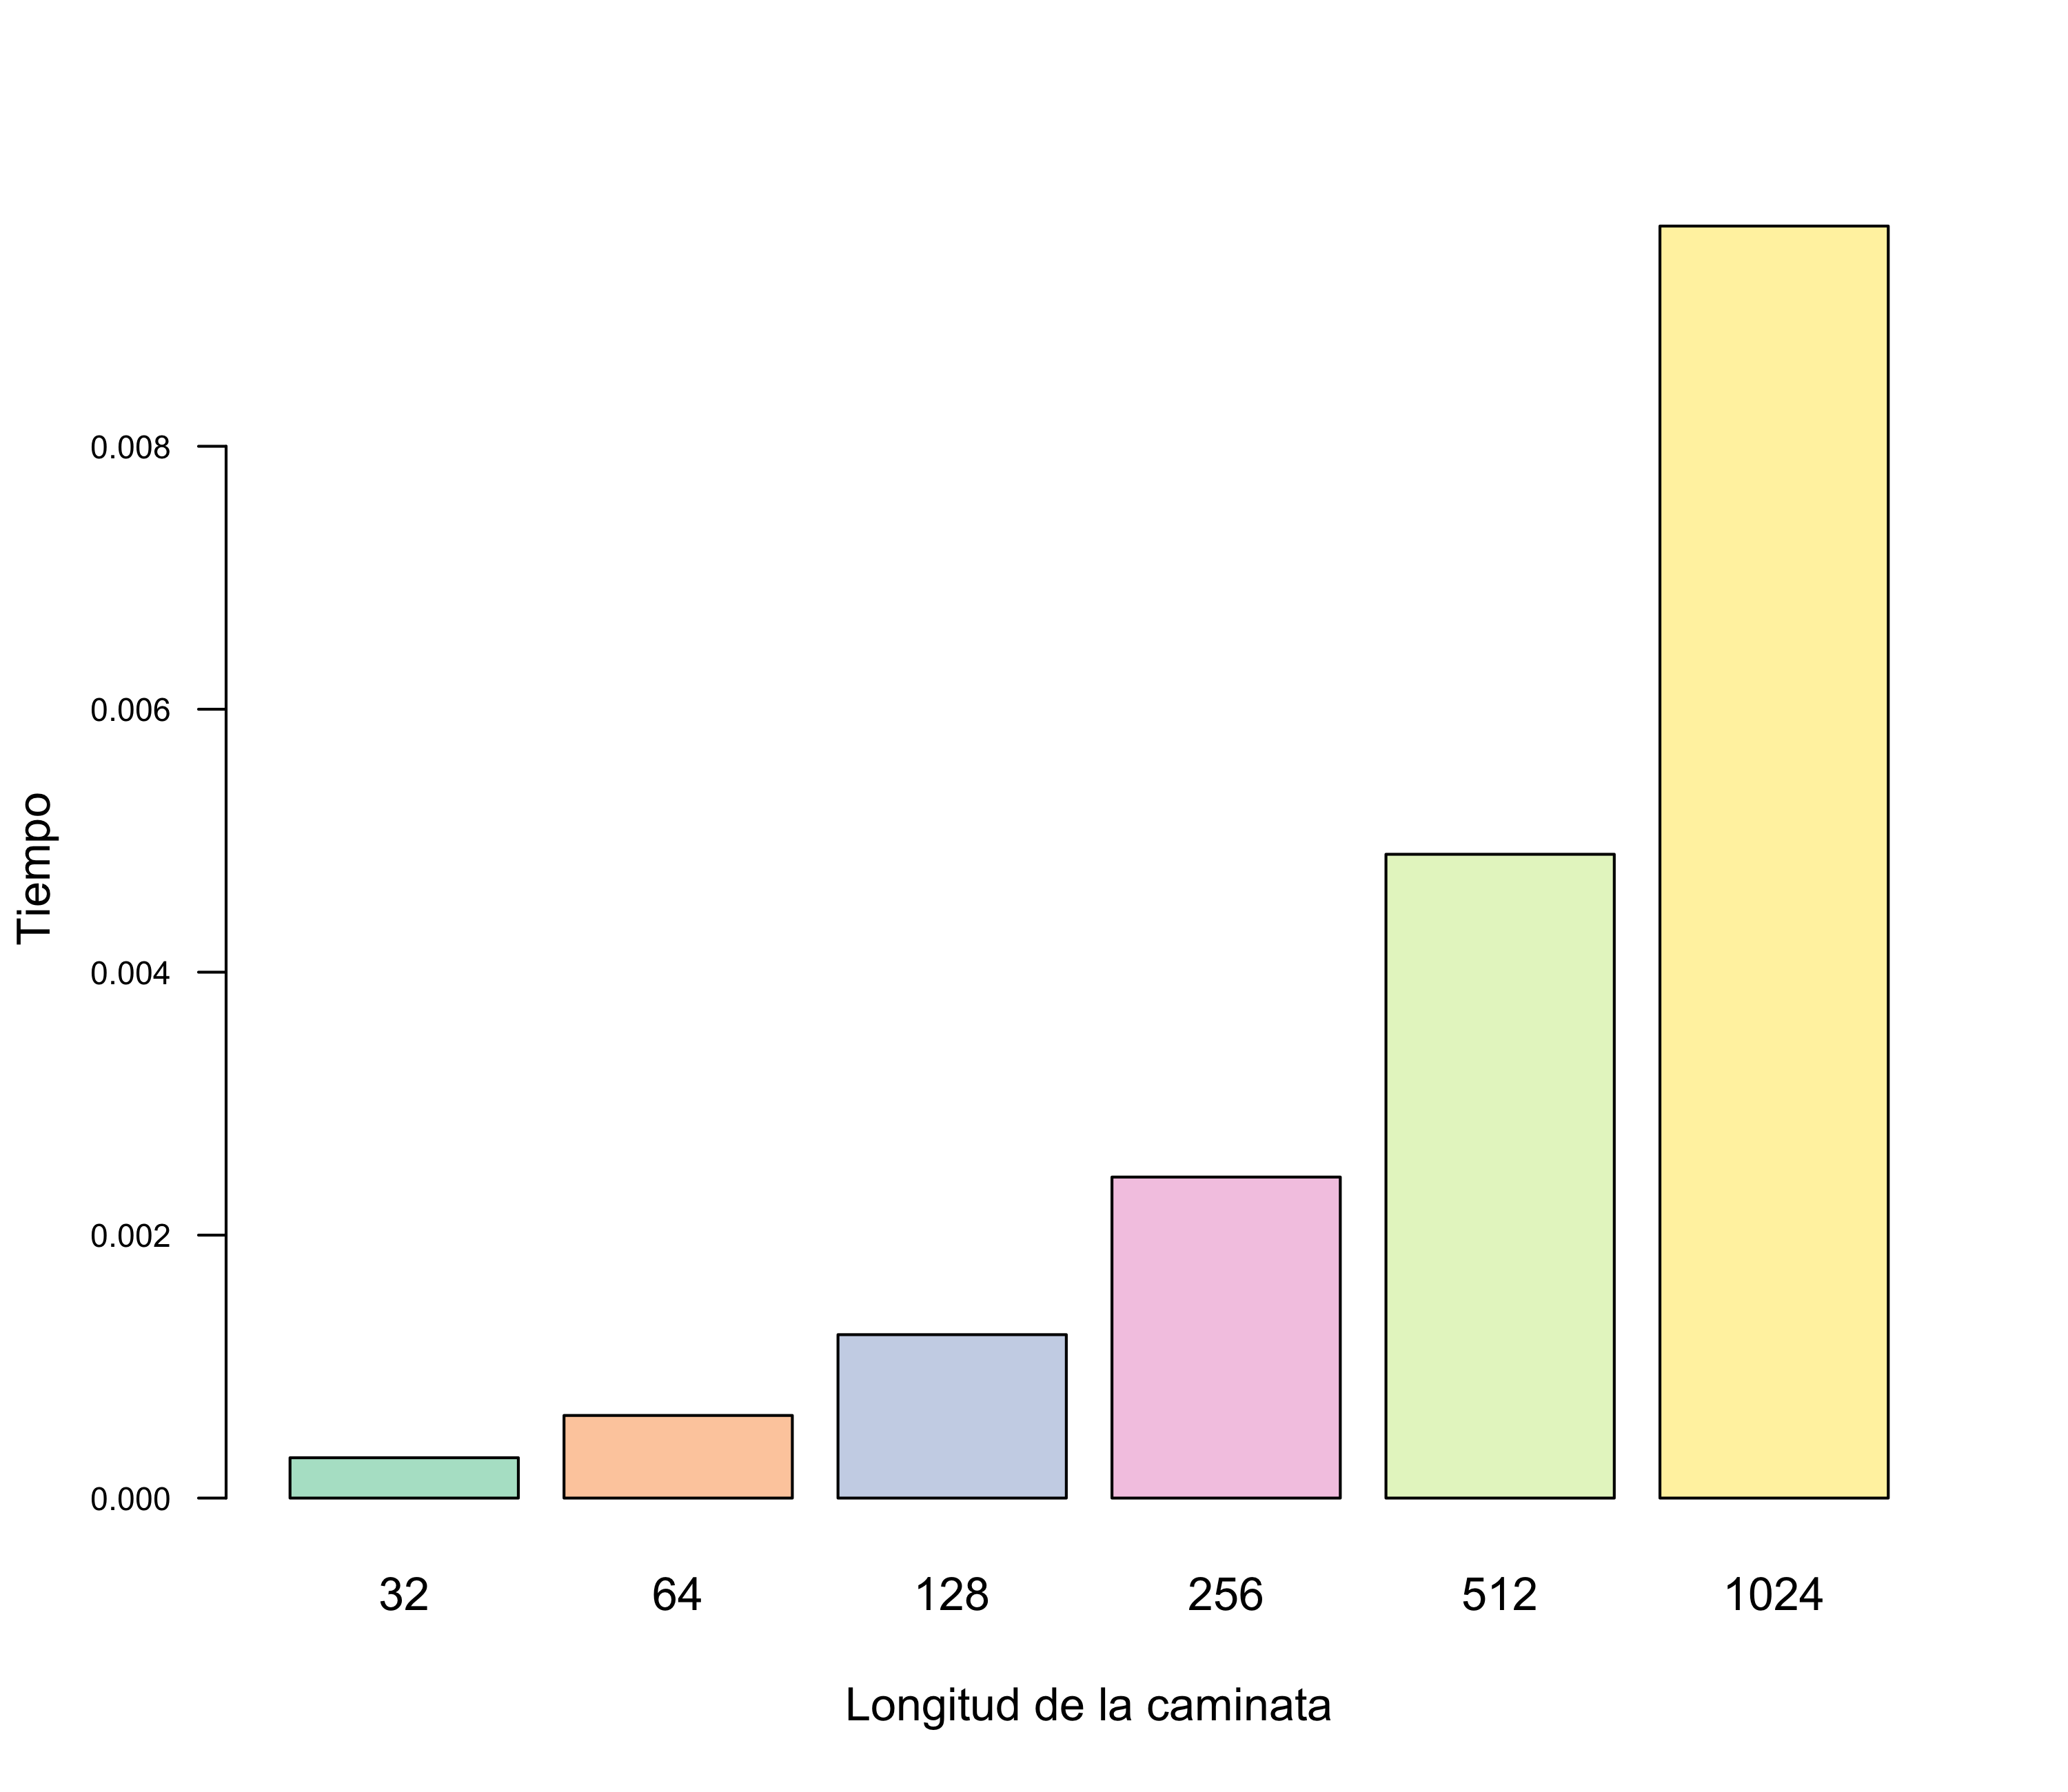
\includegraphics[width=\linewidth]{dimension6-tiempo.png}
 		 \caption{Dimensión 6.}
 		 \label{tiempos-dim6}
 	 \end{subfigure}
 		 \begin{subfigure}[b]{0.3\linewidth} 		
 		 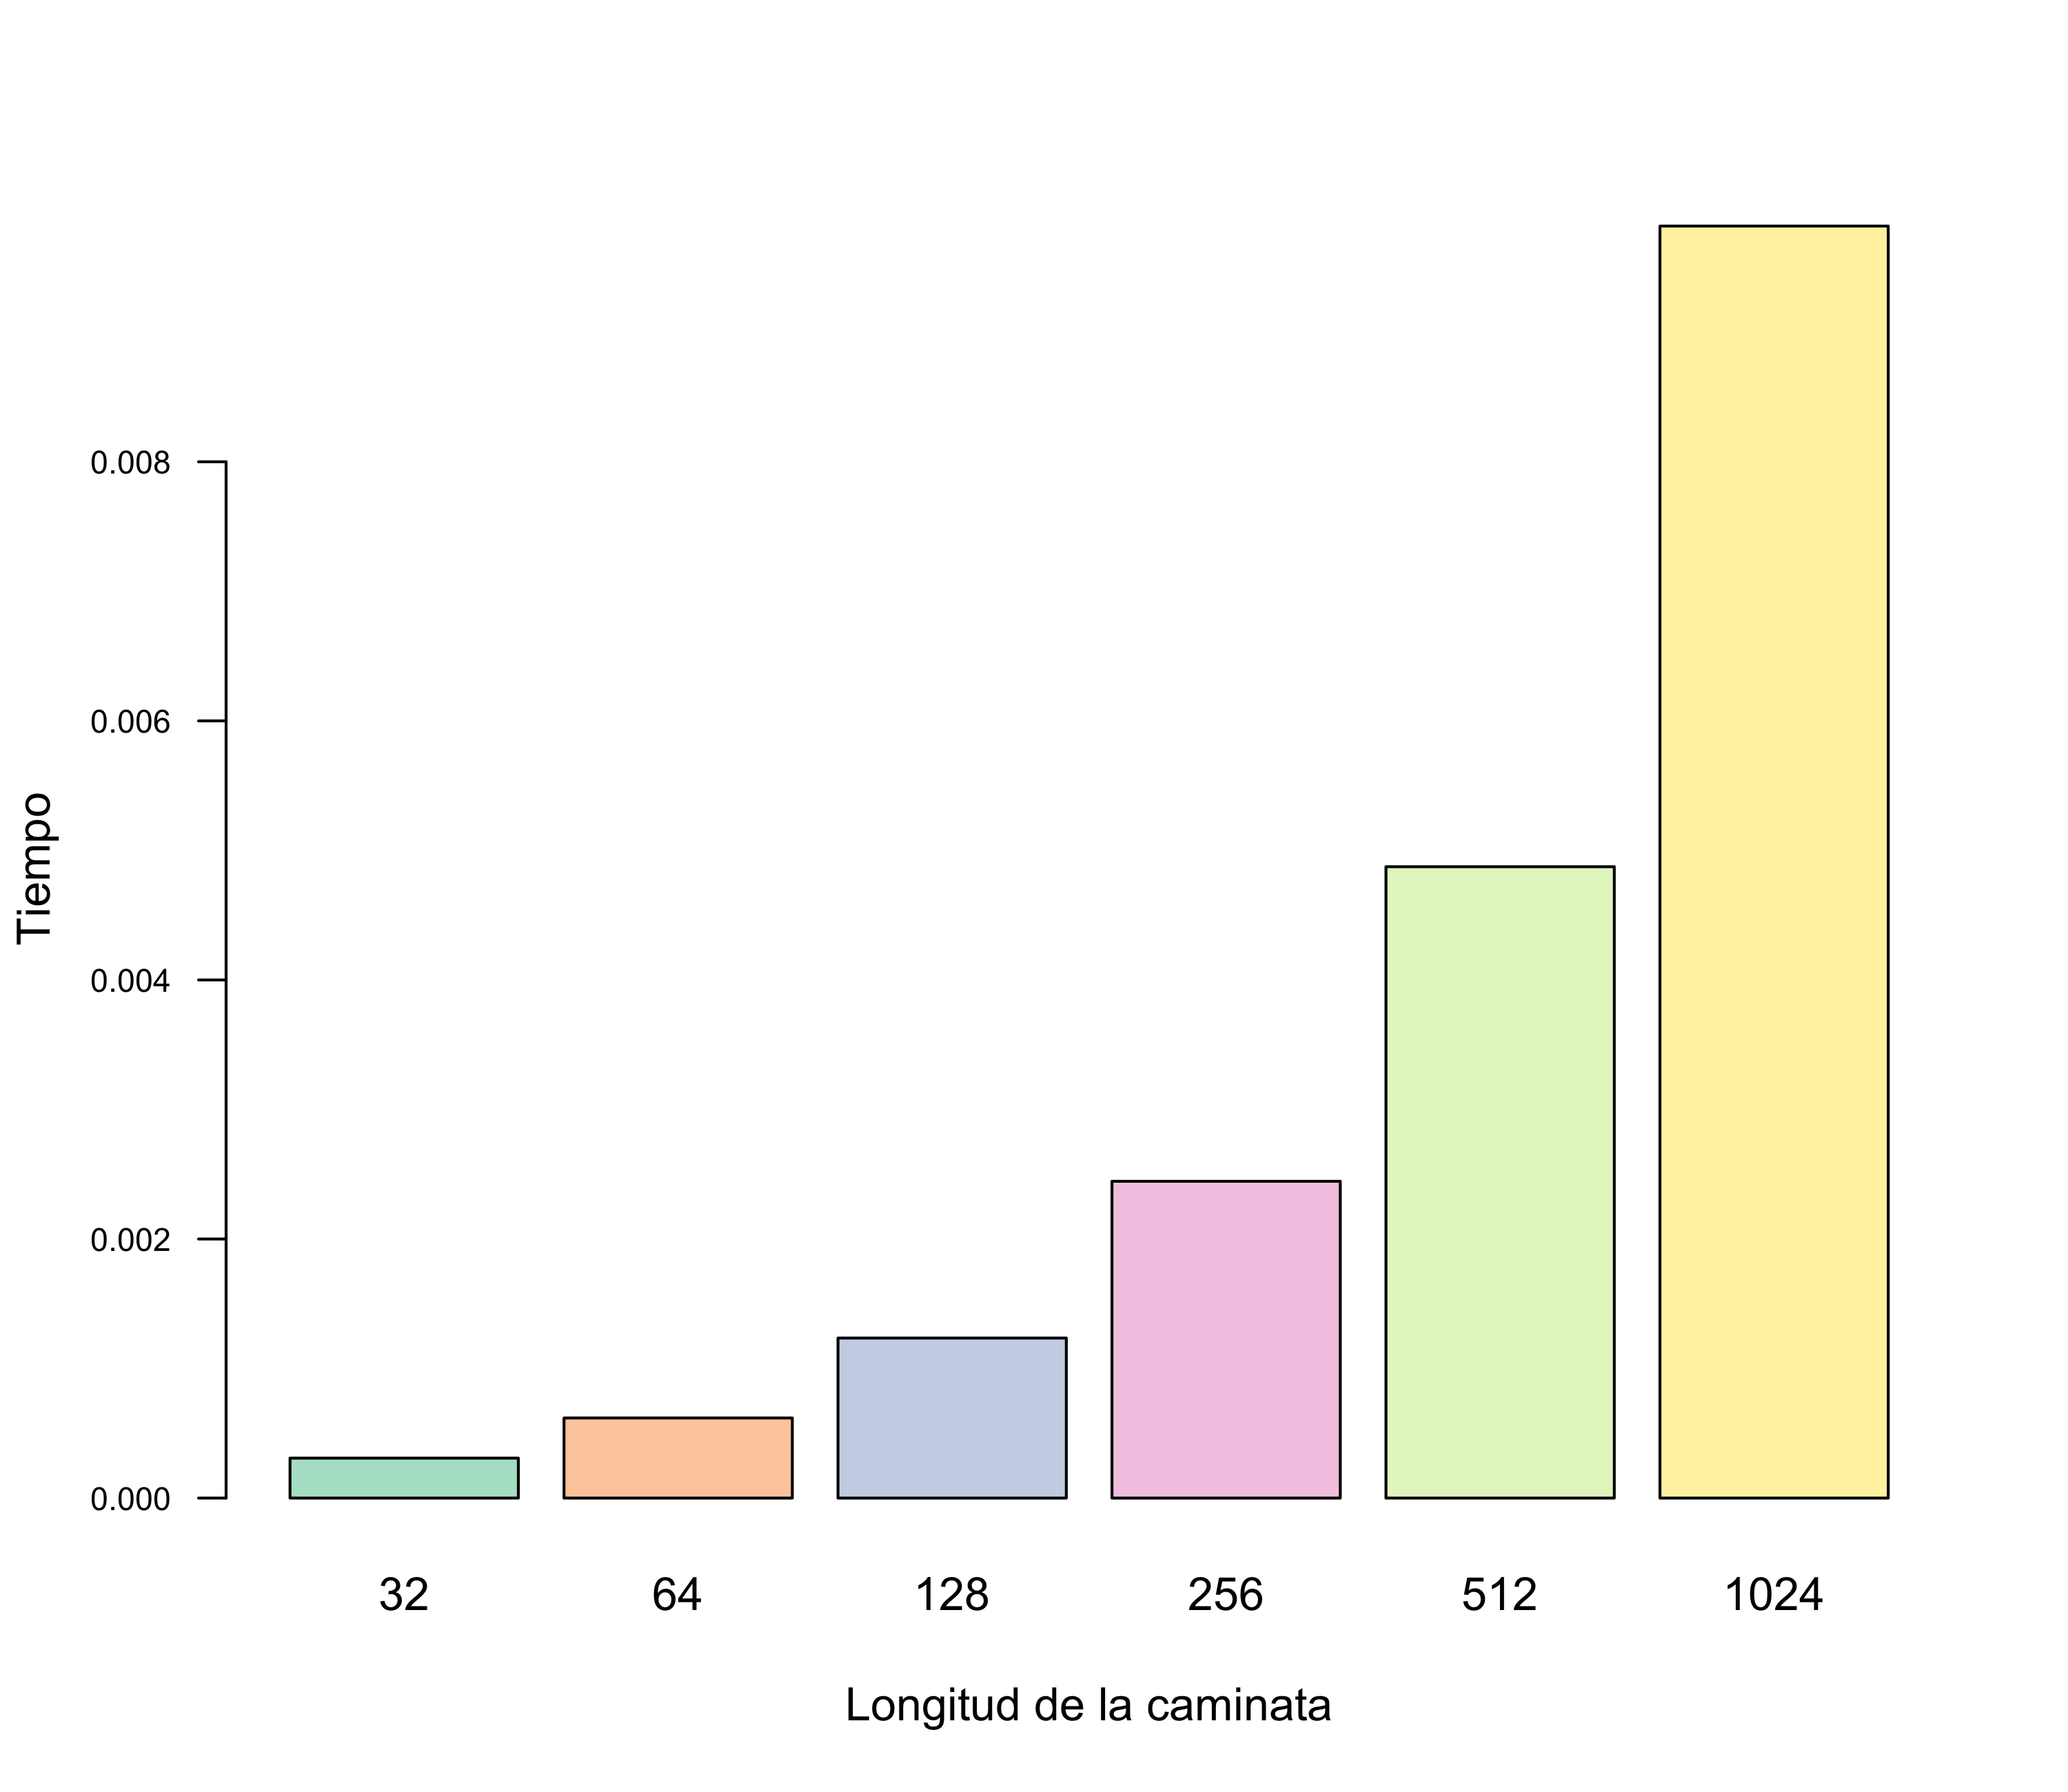
\includegraphics[width=\linewidth]{dimension7-tiempo.png}
 		 \caption{Dimensión 7.}
 		 \label{tiempos-dim7}
 	 \end{subfigure}
 		 \begin{subfigure}[b]{0.3\linewidth}
 		 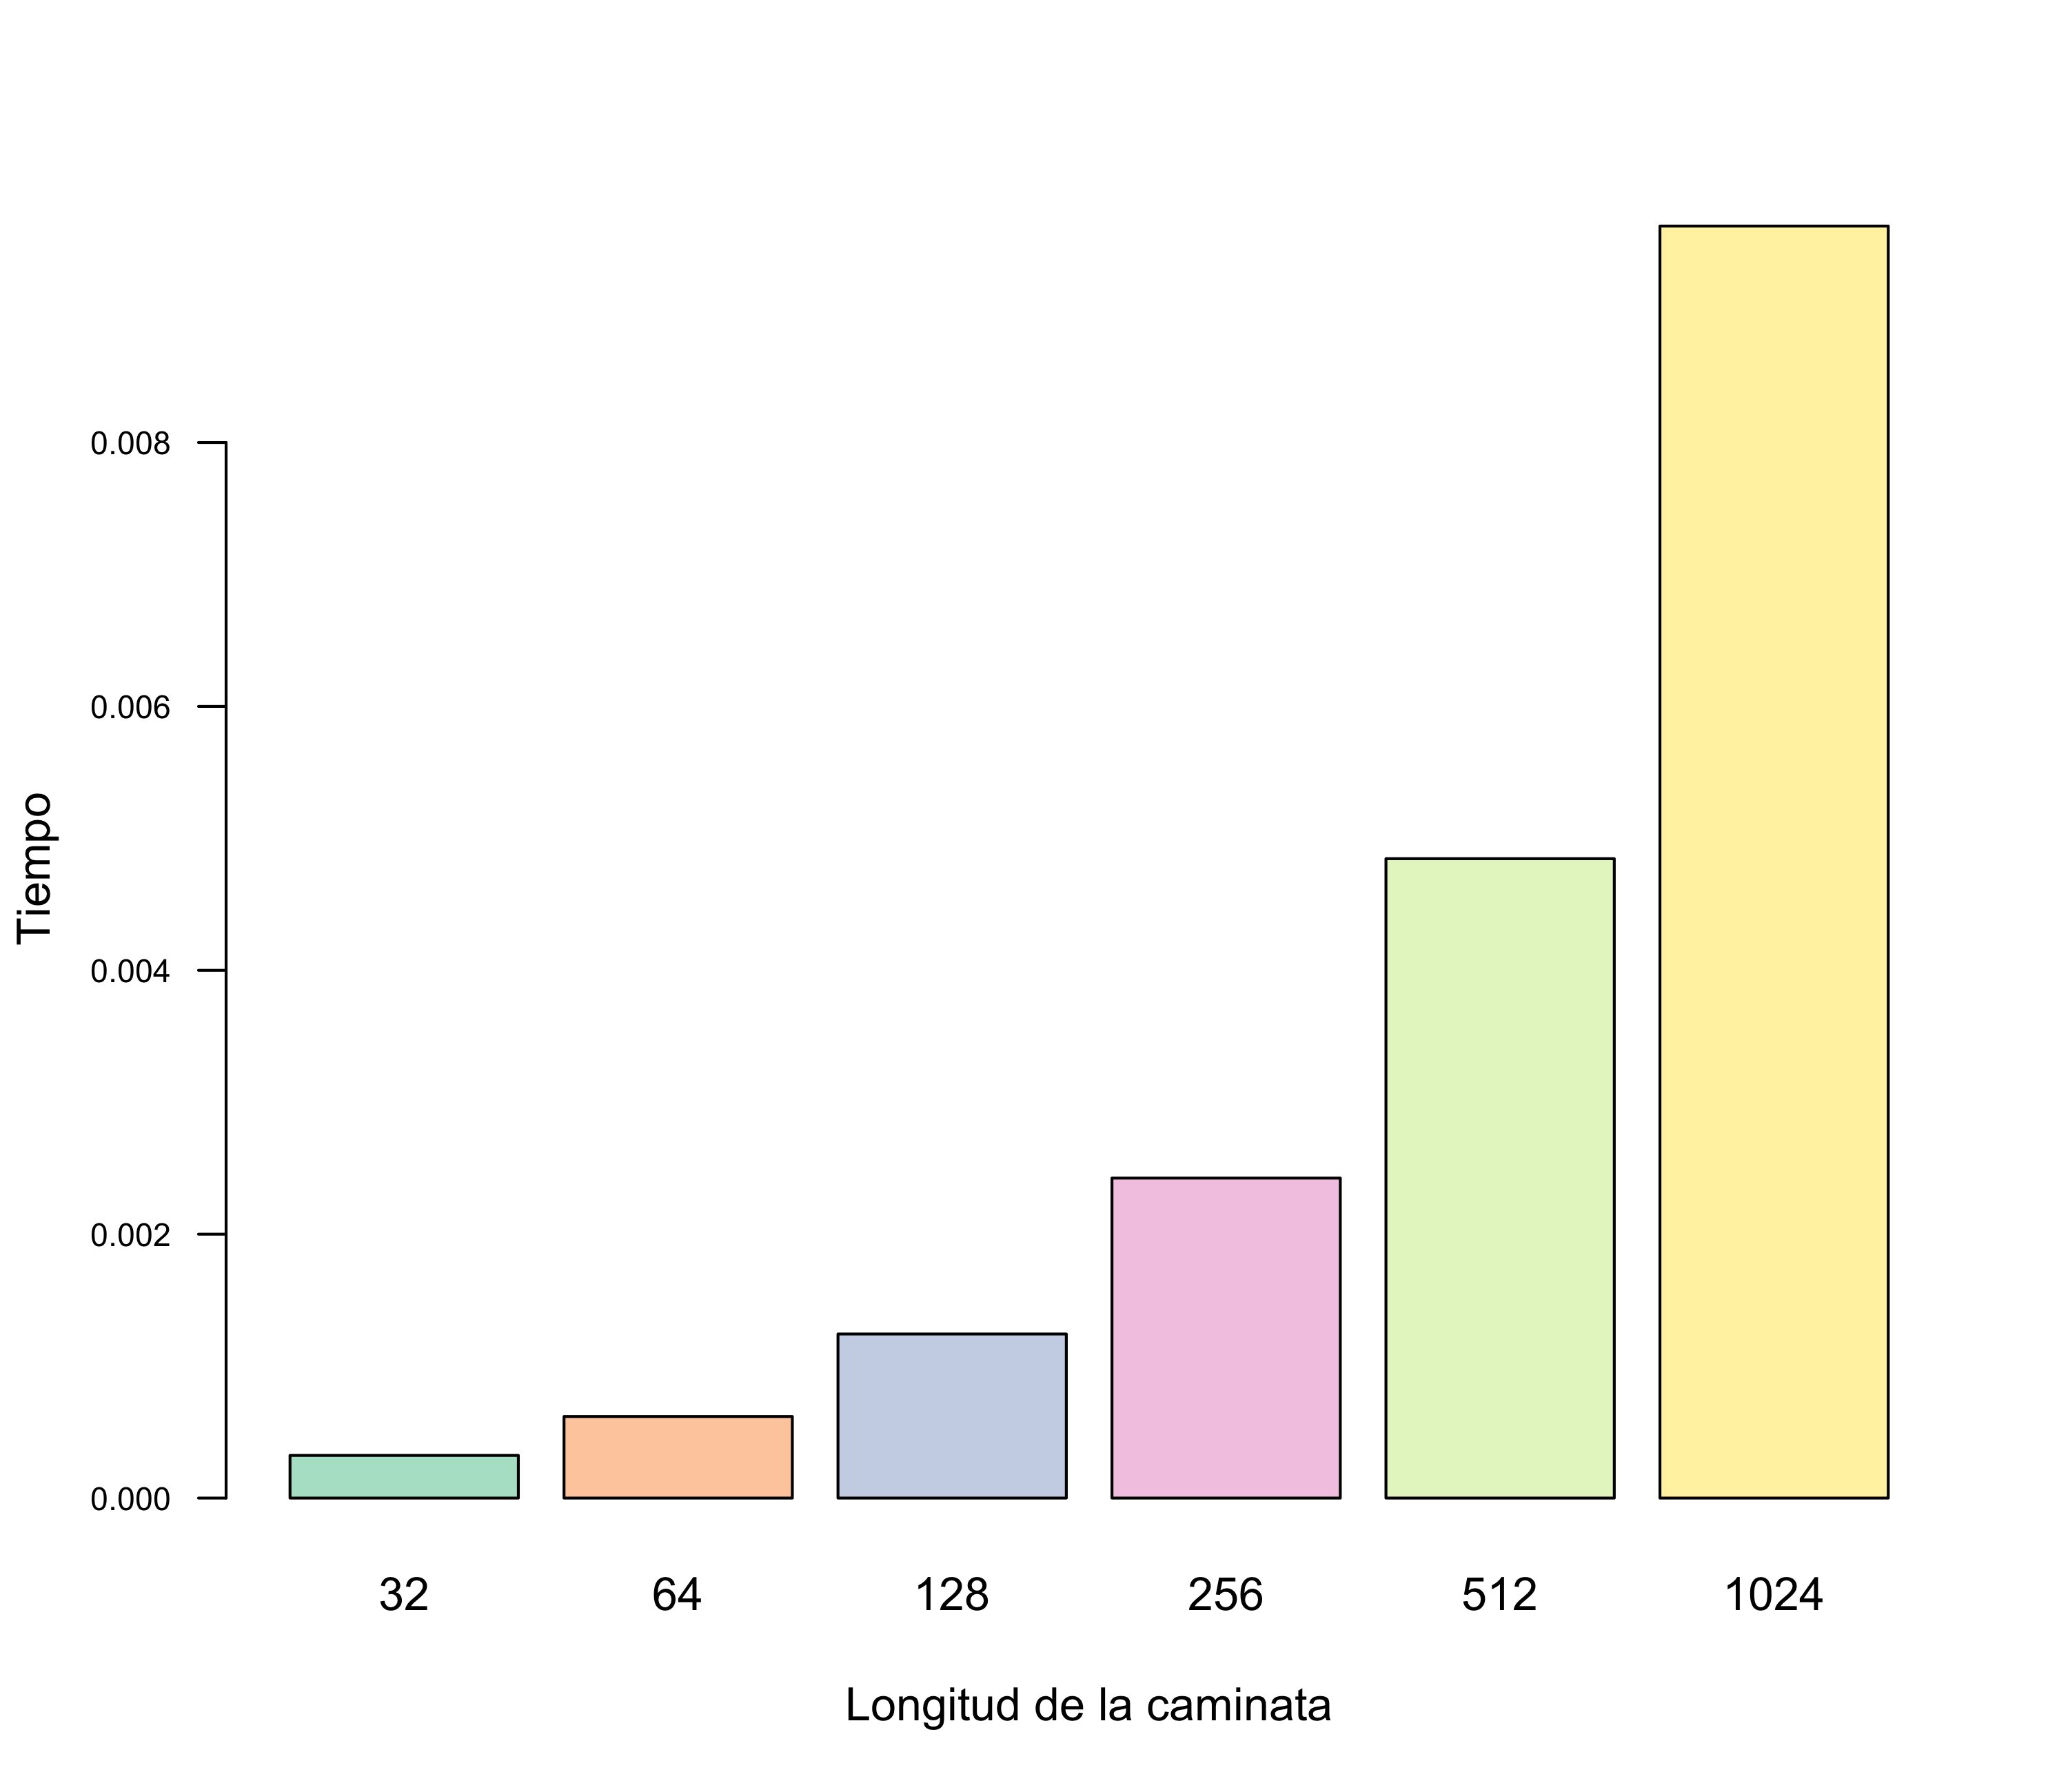
\includegraphics[width=\linewidth]{dimension8-tiempo.png}
 	 	\caption{Dimensión 8.}
 	 	\label{tiempos-dim8}
  	\end{subfigure}
  	\caption{Tiempos dependiendo de la longitud de la caminata, variando las dimensiones.}
  	  \label{tiempos-dimension}
  \end{figure}
  
  
  
\bibliographystyle{plain}
\bibliography{Referencias}

\end{document}